% Template for PLoS
% Version 3.6 Aug 2022
%
% % % % % % % % % % % % % % % % % % % % % %
%
% -- IMPORTANT NOTE
%
% This template contains comments intended 
% to minimize problems and delays during our production 
% process. Please follow the template instructions
% whenever possible.
%
% % % % % % % % % % % % % % % % % % % % % % % 
%
% Once your paper is accepted for publication, 
% PLEASE REMOVE ALL TRACKED CHANGES in this file 
% and leave only the final text of your manuscript. 
% PLOS recommends the use of latexdiff to track changes during review, as this will help to maintain a clean tex file.
% Visit https://www.ctan.org/pkg/latexdiff?lang=en for info or contact us at latex@plos.org.
%
%
% There are no restrictions on package use within the LaTeX files except that no packages listed in the template may be deleted.
%
% Please do not include colors or graphics in the text.
%
% The manuscript LaTeX source should be contained within a single file (do not use \input, \externaldocument, or similar commands).
%
% % % % % % % % % % % % % % % % % % % % % % %
%
% -- FIGURES AND TABLES
%
% Please include tables/figure captions directly after the paragraph where they are first cited in the text.
%
% DO NOT INCLUDE GRAPHICS IN YOUR MANUSCRIPT
% - Figures should be uploaded separately from your manuscript file. 
% - Figures generated using LaTeX should be extracted and removed from the PDF before submission. 
% - Figures containing multiple panels/subfigures must be combined into one image file before submission.
% For figure citations, please use "Fig" instead of "Figure".
% See http://journals.plos.org/plosone/s/figures for PLOS figure guidelines.
%
% Tables should be cell-based and may not contain:
% - spacing/line breaks within cells to alter layout or alignment
% - do not nest tabular environments (no tabular environments within tabular environments)
% - no graphics or colored text (cell background color/shading OK)
% See http://journals.plos.org/plosone/s/tables for table guidelines.
%
% For tables that exceed the width of the text column, use the adjustwidth environment as illustrated in the example table in text below.
%
% % % % % % % % % % % % % % % % % % % % % % % %
%
% -- EQUATIONS, MATH SYMBOLS, SUBSCRIPTS, AND SUPERSCRIPTS
%
% IMPORTANT
% Below are a few tips to help format your equations and other special characters according to our specifications. For more tips to help reduce the possibility of formatting errors during conversion, please see our LaTeX guidelines at http://journals.plos.org/plosone/s/latex
%
% For inline equations, please be sure to include all portions of an equation in the math environment.  For example, x$^2$ is incorrect; this should be formatted as $x^2$ (or $\mathrm{x}^2$ if the romanized font is desired).
%
% Do not include text that is not math in the math environment. For example, CO2 should be written as CO\textsubscript{2} instead of CO$_2$.
%
% Please add line breaks to long display equations when possible in order to fit size of the column. 
%
% For inline equations, please do not include punctuation (commas, etc) within the math environment unless this is part of the equation.
%
% When adding superscript or subscripts outside of brackets/braces, please group using {}.  For example, change "[U(D,E,\gamma)]^2" to "{[U(D,E,\gamma)]}^2". 
%
% Do not use \cal for caligraphic font.  Instead, use \mathcal{}
%
% % % % % % % % % % % % % % % % % % % % % % % % 
%
% Please contact latex@plos.org with any questions.
%
% % % % % % % % % % % % % % % % % % % % % % % %

\documentclass[10pt,letterpaper]{article}
\usepackage[top=0.85in,left=2.75in,footskip=0.75in]{geometry}

% amsmath and amssymb packages, useful for mathematical formulas and symbols
\usepackage{amsmath,amssymb}
\usepackage{newunicodechar}
\newunicodechar{Δ}{\Delta}
\DeclareUnicodeCharacter{03B2}{\textbeta}
\newunicodechar{₂}{$_2$}
\newunicodechar{ }{~}
\newunicodechar{ }{\,}

% Use adjustwidth environment to exceed column width (see example table in text)
\usepackage{changepage}

% textcomp package and marvosym package for additional characters
\usepackage{textcomp,marvosym}

% cite package, to clean up citations in the main text. Do not remove.
\usepackage{natbib} % for \citep and \citet
% \usepackage{cite} % comment out or remove if using natbib

% Use nameref to cite supporting information files (see Supporting Information section for more info)
\usepackage{nameref,hyperref}

% line numbers
\usepackage[right]{lineno}

% ligatures disabled
\usepackage[nopatch=eqnum]{microtype}
\DisableLigatures[f]{encoding = *, family = * }

% color can be used to apply background shading to table cells only
\usepackage[table]{xcolor}
\usepackage{enumitem}
\usepackage{booktabs}

% array package and thick rules for tables
\usepackage{array}

% create "+" rule type for thick vertical lines
\newcolumntype{+}{!{\vrule width 2pt}}

% create \thickcline for thick horizontal lines of variable length
\newlength\savedwidth
\newcommand\thickcline[1]{%
  \noalign{\global\savedwidth\arrayrulewidth\global\arrayrulewidth 2pt}%
  \cline{#1}%
  \noalign{\vskip\arrayrulewidth}%
  \noalign{\global\arrayrulewidth\savedwidth}%
}

% \thickhline command for thick horizontal lines that span the table
\newcommand\thickhline{\noalign{\global\savedwidth\arrayrulewidth\global\arrayrulewidth 2pt}%
\hline
\noalign{\global\arrayrulewidth\savedwidth}}


% This is for Supplementary
\usepackage{graphicx}      % already in almost every template
\usepackage{subcaption}    % gives sub-figures + \subref
\usepackage{placeins}      % lets us slam a barrier before the SI
\usepackage[margin=1in]{geometry}

% For table
\usepackage{booktabs}
\usepackage{multirow}
\usepackage{array}
\usepackage{tabularx}

% ---------- helper to switch counters to S-numbers ----------
\newcommand{\beginsupplement}{%
  \setcounter{table}{0}%
  \renewcommand{\thetable}{S\arabic{table}}%
  \setcounter{figure}{0}%
  \renewcommand{\thefigure}{S\arabic{figure}}}

% 2) Define a macro \beginsupplement that:
%    • Resets the figure/table counters
%    • Prefixes future figures/tables with “S”
\usepackage{etoolbox} % for \pretocmd and \setcounter


% Remove comment for double spacing
%\usepackage{setspace} 
%\doublespacing

% Text layout
\raggedright
\setlength{\parindent}{0.5cm}
\textwidth 5.25in 
\textheight 8.75in

% Bold the 'Figure #' in the caption and separate it from the title/caption with a period
% Captions will be left justified
\usepackage[aboveskip=1pt,labelfont=bf,labelsep=period,justification=raggedright,singlelinecheck=off]{caption}
\renewcommand{\figurename}{Fig}

% Use the PLoS provided BiBTeX style


% Remove brackets from numbering in List of References
\makeatletter
\renewcommand{\@biblabel}[1]{\quad#1.}
\makeatother

% links
\usepackage{hyperref}


% Header and Footer with logo
\usepackage{lastpage,fancyhdr,graphicx}
\usepackage{epstopdf}
%\pagestyle{myheadings}
\pagestyle{fancy}
\fancyhf{}
%\setlength{\headheight}{27.023pt}
%\lhead{\includegraphics[width=2.0in]{PLOS-submission.eps}}
\rfoot{\thepage/\pageref{LastPage}}
\renewcommand{\headrulewidth}{0pt}
\renewcommand{\footrule}{\hrule height 2pt \vspace{2mm}}
\fancyheadoffset[L]{2.25in}
\fancyfootoffset[L]{2.25in}
\lfoot{\today}

%% Include all macros below

\newcommand{\lorem}{{\bf LOREM}}
\newcommand{\ipsum}{{\bf IPSUM}}



%% END MACROS SECTION
\usepackage{graphicx}
\usepackage[aboveskip=1pt,labelfont=bf,labelsep=period,justification=raggedright,singlelinecheck=off]{caption}
\usepackage{placeins}

\begin{document}
\vspace*{0.2in}

% Title must be 250 characters or less.
\begin{flushleft}
{\Large
\textbf\newline{Sorghum Lipidomics Database} % Please use "sentence case" for title and headings (capitalize only the first word in a title (or heading), the first word in a subtitle (or subheading), and any proper nouns).
}
\newline
% Insert author names, affiliations and corresponding author email (do not include titles, positions, or degrees).
\\
Nirwan Tandukar\textsuperscript{1,2\Yinyang},
Ruthie Stokes\textsuperscript{3},
Name4 Surname\textsuperscript{2},
Name5 Surname\textsuperscript{2\ddag},
Name6 Surname\textsuperscript{2\ddag},
Rubén Rellán Álvarez\textsuperscript{1,3*},

\bigskip
\textbf{1} Department of Genetics and Genomics, North Carolina State University, Raleigh, NC, USA
\\
\textbf{2} Department of Bioinformatics, North Carolina State University, Raleigh, NC, USA
\\
\textbf{3} Department of Molecular and Structural Biochemistry,  North Carolina State University, Raleigh, NC, USA
\\
\bigskip


% Insert additional author notes using the symbols described below. Insert symbol callouts after author names as necessary.
% 
% Remove or comment out the author notes below if they aren't used.
%
% Primary Equal Contribution Note
\Yinyang These authors contributed equally to this work.

% Additional Equal Contribution Note
% Also use this double-dagger symbol for special authorship notes, such as senior authorship.
\ddag These authors also contributed equally to this work.

% Current address notes
\textcurrency Current Address: Dept/Program/Center, Institution Name, City, State, Country % change symbol to "\textcurrency a" if more than one current address note
% \textcurrency b Insert second current address 
% \textcurrency c Insert third current address



% Group/Consortium Author Note
\textpilcrow Membership list can be found in the Acknowledgments section.

% Use the asterisk to denote corresponding authorship and provide email address in note below.
* correspondingauthor@institute.edu

\end{flushleft}
% Please keep the abstract below 300 words
\section*{Abstract}
SAP lines



\linenumbers

% Use "Eq" instead of "Equation" for equation citations.
\section*{Introduction}

\subsection*{Lipid remodelling under abiotic constraints}

Plants remodel their membranes in a highly‐orchestrated manner when temperature or nutrient supply is sub‑optimal.  Below we summarise the characteristic fingerprints for \textbf{cold}, \textbf{phosphorus} and \textbf{nitrogen} stress, with emphasis on (i) class ratios that can be used as diagnostic indicators and (ii) individual molecular species that act as markers in lipidomic data sets.

%--------------------------------------------------------------------
\subsubsection*{Cold stress}
\label{sec:cold}

\begin{enumerate}[label=\textbf{\arabic*.}, leftmargin=1.2em]
  \item \textbf{Higher acyl‑chain unsaturation.}  Cold‐tolerant genotypes accumulate poly‑unsaturated fatty acids—principally 18\,:3, 18\,:2 and 18\,:1—leading to a higher double‑bond index (DBI) and preventing membrane rigidification at low temperature \citep[pp.~431–440, 460]{Low_temp_stress_Bhattacharya}.  An increase in DBI is consistently reported in tolerant lines of \textit{Arabidopsis}, maize and peanut \citep[pp.~11–12]{Lipid_transcriptome_Cold_stress_Yu}.

  \item \textbf{Class‑level reshaping.}  
        \begin{itemize}
          \item Poly‑unsaturated PC, PE, PG, MGDG and DGDG species rise, whereas their saturated counterparts decline \citep[pp.~3–4]{Low_temperatures_Wang,Low_temp_stress_Bhattacharya}.  
          \item The bilayer/non‑bilayer ratio, \(\mathrm{(PC+DGDG)/(PE+MGDG)}\), increases, stabilising the lamellar phase of membranes during freezing events \citep[pp.~492–493]{Low_temp_stress_Bhattacharya}.  
          \item Phosphatidic acid (PA) and lysophospholipids (LPC, LPE) surge, reflecting activation of phospholipase D and A, respectively \citep[pp.~456, 472--474]{Low_temp_stress_Bhattacharya}.
        \end{itemize}

  \item \textbf{Species‑level markers.}  In maize, PA\,36:5, PA\,36:6, DAG\,36:5 and DAG\,36:6 are elevated, whereas MGDG\,36:5 and multiple PC species decline \citep[pp.~6–8]{cold_tolerance_maize_Shi}.  Tolerant cultivars show higher TAG and lower DAG/TAG ratios compared with sensitive lines \citep[pp.~11]{Lipid_transcriptome_Cold_stress_Yu}.

  \item \textbf{Lipid signalling.}  PLD- and PLA‑derived PA and lyso‑lipids act as second messengers, triggering cold‐responsive gene networks \citep[pp.~454–456]{Low_temp_stress_Bhattacharya}.

  \item \textbf{Functional outcome.}  Increased unsaturation and altered bilayer propensity maintain a fluid–crystalline phase, securing electron transport and nutrient transport across membranes at low temperature \citep[pp.~463–465]{Low_temp_stress_Bhattacharya}.
\end{enumerate}

%--------------------------------------------------------------------
\subsubsection*{Phosphorus deprivation}
\label{sec:phosphorus}

\begin{enumerate}[label=\textbf{\arabic*.}, leftmargin=1.2em]
  \item \textbf{Phospholipid depletion.}  Major phospholipids (PC, PE, PG, PI, PS, PA) decline sharply as they serve as an internal Pi source; in soybean leaves every phospholipid class decreased under Pi limitation \citep[pp.~1,\,3,\,5]{lipid_remodeling_low_P_Saito}.

  \item \textbf{Compensatory rise of non‑P lipids.}  MGDG, DGDG, SQDG and the diagnostic glucuronosyldiacylglycerol (GlcADG) accumulate to preserve membrane surface area \citep[pp.~3--4]{Phosphate_deficiency_Wang}.  GlcADG can increase up to 14‑fold in soybean \citep{lipid_remodeling_low_P_Saito}.

  \item \textbf{Diagnostic ratio.}  The phospholipid/galactolipid ratio (PL/GL) drops from \(\sim\)0.3 (P‐sufficient) to \(\le 0.05\) under severe P stress in field‐grown camelina \citep[page~4]{Phosphate_deficiency_Wang}.

  \item \textbf{Tissue specificity.}  Older leaves are remodelled first, exporting Pi to developing tissues \citep[pp.~1,\,5]{lipid_remodeling_low_P_Saito}.

  \item \textbf{Enzymatic drivers.}  Phospholipase C/D hydrolyse PC and PE; MGDG/DGDG and SQDG synthases are up‑regulated to supply the replacement lipids \citep[pp.~1–2, 6]{Phosphate_scaracity_Xue}.
\end{enumerate}

%--------------------------------------------------------------------
\subsubsection*{Nitrogen deprivation}
\label{sec:nitrogen}

\begin{enumerate}[label=\textbf{\arabic*.}, leftmargin=1.2em]
  \item \textbf{Chloroplast glycolipids.}  Rapeseed shows an 18 % (leaf) to 35 % (root) reduction in MGDG; DGDG declines by 23 % in roots, resulting in a suppressed \(\mathrm{MGDG/DGDG}\) ratio \citep[pp.~5--9]{nitrogen_deficiency_lipid_Yang}.

  \item \textbf{Phospholipid curtailment.}  PC, PE, PI, PS and PA all decrease markedly, the latter by more than 90 % in both organs \citep{nitrogen_deficiency_lipid_Yang}.

  \item \textbf{Storage lipids.}  TAG remains unchanged in rapeseed but accumulates in mature tea leaves under low N, suggesting carbon re‑allocation from photosynthetic (N‑rich) to storage pools \citep[pp.~6--7]{Nitrogen_fertilizer_Ruan}.

  \item \textbf{Integrated carbon‑nitrogen balance.}  Lower nitrogen leaves a surplus of assimilated carbon; plants divert it into TAG or into highly unsaturated MGDG 36:5/36:6 species observed in tea shoots at high N \citep{Nitrogen_fertilizer_Ruan}.
\end{enumerate}

%--------------------------------------------------------------------
\subsubsection*{Synthesis}

Cold, P and N stress each trigger a distinctive yet overlapping pattern of lipid remodelling:

\begin{itemize}
  \item \textbf{Cold} prioritises \emph{unsaturation} and bilayer‑to‑non‑bilayer balance to maintain fluidity.  
  \item \textbf{Pi starvation} reallocates phosphorus by replacing phospho‑lipids with galacto‑ and sulfo‑lipids, sharply lowering the PL/GL ratio.  
  \item \textbf{N starvation} down‑regulates chloroplast glycolipids and phospholipids, sometimes storing excess carbon as TAG.  
\end{itemize}

These shifts are mirrored in our sorghum data: unsaturation indices rise under early low‑temperature planting; the \(\mathrm{DGDG/MGDG}\) and \(\mathrm{SQDG/PG}\) ratios increase under P‑limited, low‑input conditions; and TAG/PC as well as \(\mathrm{TG/DG}\) ratios escalate when available nitrogen is low (see Sections \ref{sec:cold}, \ref{sec:phosphorus} and \ref{sec:nitrogen}).

- Stress in plants specifically in sorghum

- Cold stress

- low Nitrogen

- low Phosphorus

- Relate to climate change?



%---------------------------------------------------------------
\begin{table}[ht]
\centering
\small
\setlength{\tabcolsep}{6pt}
\renewcommand{\arraystretch}{1.15}
\begin{tabular}{@{}p{2.3cm} p{4.2cm} p{1.3cm} p{4.5cm} p{1.7cm}@{}}
\toprule
\textbf{Stress} & \textbf{Key lipid class / molecular species} & \textbf{Direction\textsuperscript{a}} & \textbf{Diagnostic (ratio) or remark} & \textbf{Ref.} \\
\midrule
\multirow{6}{*}{\textbf{Cold}} 
 & Poly‑unsaturated FA (18:3, 18:2, 18:1)            & $\uparrow$ & Higher double‑bond index (DBI)                                & \citet{Low_temp_stress_Bhattacharya} \\
 & Unsat.\ PC, PE, PG, MGDG, DGDG                     & $\uparrow$ & Bilayer lipids enriched                                        & \citet{Low_temperatures_Wang}        \\
 & PA (incl.\ PA\,36:5;\,36:6)                        & $\uparrow$ & PLD activation; signalling                                     & \citet{cold_tolerance_maize_Shi}     \\
 & LPC, LPE                                           & $\uparrow$ & PLA activity                                                   & \citet{Low_temp_stress_Bhattacharya} \\
 & DAG\,36:5;\,36:6                                   & $\uparrow$ & Mobilisation of PC unsat.\ chains                             & \citet{cold_tolerance_maize_Shi}     \\
 & TAG (total)                                        & $\uparrow$ & \textit{cf.}\ DAG/TAG $\downarrow$ in tolerant lines           & \citet{Lipid_transcriptome_Cold_stress_Yu} \\
 \cmidrule{2-5}
 & \multicolumn{2}{@{}l}{\textit{Cold ratios}}       & (PC\,+\,DGDG)/(PE\,+\,MGDG)\:$\uparrow$; \ DAG/TAG\:$\downarrow$ & \citet{Low_temp_stress_Bhattacharya} \\
\midrule
\multirow{5}{*}{\textbf{P deficiency}} 
 & PC, PE, PG, PI, PS, PA                             & $\downarrow$ & Release of Pi pool                                            & \citet{lipid_remodeling_low_P_Saito} \\
 & MGDG, DGDG                                          & $\uparrow$  & Galacto‑lipid replacement                                     & \citet{Phosphate_deficiency_Wang}    \\
 & SQDG                                               & $\uparrow$  & Sulfo‑lipid substitution                                      & \citet{Phosphate_deficiency_Wang}    \\
 & GlcADG                                             & $\uparrow$  & Pi‑stress biomarker (14‑fold)                                 & \citet{lipid_remodeling_low_P_Saito} \\
 & \multicolumn{2}{@{}l}{\textit{P ratios}}           & PL/GL $\downarrow$ (to $\le$ 0.05); DGDG/MGDG $\uparrow$        & \citet{Phosphate_deficiency_Wang}    \\
\midrule
\multirow{5}{*}{\textbf{N deficiency}} 
 & MGDG (leaf, root)                                  & $\downarrow$ & 18–35 \% reduction                                            & \citet{nitrogen_deficiency_lipid_Yang} \\
 & DGDG (root)                                        & $\downarrow$ & 24 \% reduction                                               & \citet{nitrogen_deficiency_lipid_Yang} \\
 & PC, PE, PI, PS, PA                                 & $\downarrow$ & PA $\downarrow$ > 90 \%                                       & \citet{nitrogen_deficiency_lipid_Yang} \\
 & TAG (mature tea leaves)                            & $\uparrow$  & Carbon sink under low N                                       & \citet{Nitrogen_fertilizer_Ruan}      \\
 & \multicolumn{2}{@{}l}{\textit{N ratios}}           & MGDG/DGDG $\downarrow$; TAG/PC $\uparrow$; TG/DG $\uparrow$     & \citet{nitrogen_deficiency_lipid_Yang} \\
\bottomrule
\multicolumn{5}{l}{\footnotesize \textsuperscript{a}\,$\uparrow$ increase, $\downarrow$ decrease relative to control or sufficient nutrient.}
\end{tabular}
\caption{Core lipid markers and class ratios characterising cold, phosphorus and nitrogen stress as distilled from the literature survey.  Arrows indicate the direction of change in stressed tissues.}
\label{tab:lipid_markers}
\end{table}
%---------------------------------------------------------------


\subsection*{OPLS-DA}
4. Supervised multivariate discrimination of the lipidomes
4.1 What OPLS‑DA does—in plain language
Orthogonal‑Projection to Latent Structures Discriminant Analysis (OPLS‑DA) is a supervised extension of Principal‑Component Analysis that forces the first latent component to explain only variance that is correlated with a user‑defined class vector (here, Control vs Low‑input). Any systematic variation that is orthogonal to class membership—batch differences, genotype heterogeneity, stochastic noise—is captured in subsequent, “orthogonal” components.
The outcome is a model that

separates classes as strongly as possible along a single predictive axis (t1),

isolates uninformative variance on orthogonal axes (to1, to2, …), and

provides a Variable‑Importance in Projection (VIP) score for every lipid, ranking its contribution to class separation.

Because the method is supervised, we rigorously guard against over‑fitting by (i) k‑fold cross‑validation (Q²) and (ii) permutation testing.

4.2 Model quality and diagnostic overview (Fig. 6a–d)
<div align="center"><em>Insert composite “overview” panel here</em></div>
Panel (a) – Component summary 
The model contains one predictive component (p1) and two orthogonal components (o1, o2). Predictive component p1 alone explains 94 % of the class variance (R²Y) and 94 % of its cross‑validated predictability (Q²Y), well above the commonly accepted 0.5 threshold (grey reference line). Orthogonal components capture residual variation in the lipid matrix (R²X ≈ 0.70 in total) that is unrelated to treatment.

Panel (b) – Permutation test 
Two‑hundred random permutations of the class vector were fitted to the same data (grey dots). None of the permuted models approaches the real model’s Q² or R² (black bars on the right). The probability of obtaining an equal or better model by chance is pR²Y = 0.05; pQ² = 0.05, confirming that the discrimination is not an over‑fit artefact.

Panel (c) – Observation diagnostics 
Score‑distance (SD, leverage) is plotted against orthogonal distance (OD, residual variance). Dashed lines denote the 95 % Hotelling T² limits. Only five genotypes (labels s441, s736, s447…) exceed one or both thresholds; visual inspection of chromatograms revealed no technical issue, hence they were retained.

Panel (d) – Score plot 
Each point represents a genotype; blue = Control, red = Low‑input. The two classes form well‑separated, compact clouds along the predictive axis t1 (39 % of total lipid variance), while the orthogonal axis to1 (30 %) captures within‑class dispersion. The 95 % confidence ellipse encloses every sample except the mild outliers identified in panel (c). Together with the high Q², this demonstrates a robust lipidomic signature of the Low‑input treatment.

4.3 Discriminatory lipids revealed by VIP analysis (Fig. 6e)
<div align="center"><em>Insert VIP bar plot (top 30) here</em></div>
VIP values quantify how strongly each lipid contributes to the predictive component. A conservative cut‑off of VIP > 1.3 (dashed line) yielded 28 discriminatory species (Supplementary Table S7). The top ten are displayed in Fig. 6e and encompass several structural classes:

Rank	Lipid (annotation)	Class	VIP	Change in Low‑input†
1	Nostoxanthin	Terpenoid	1.88	 ↑ 4.1‑fold
2	Triethylene‑glycol bis(2‑ethyl‑hexanoate)	Plasticizer ‡	1.82	 ↓ 3.6‑fold
3	ε‑Decalactone	Organic compound	1.79	 ↑ 2.9‑fold
…	…	…	…	…

† Fold‑change refers to median linear intensity.
‡ Likely exogenous contaminant; retained for completeness but excluded from biological discussion.

Biologically meaningful drivers include:

Triacyl‑glycerols TG(56:6), TG(46:0) – consistently enriched under Low‑input, supporting the nitrogen‑remobilisation hypothesis (Fig. 6e, pale‑blue bars).

Phosphatidylethanolamine PE(34:1) – depleted in Low‑input, aligning with the phospholipid‑to‑glycolipid replacement model under combined low P/low N.

β‑Sitosterol – a sterol known to modulate membrane order, markedly increased (VIP 1.55), coherent with the observed membrane‑integrity ratios (Fig. 5).

These VIP‑identified species therefore corroborate and extend the univariate ratio analysis.

4.4 Interpretation
The OPLS‑DA model demonstrates that field Low‑input treatment imprints a strong, coherent lipidomic signature across 350–380 sorghum genotypes, explaining > 80 % of class variance with excellent predictability.

Discriminating lipids belong to storage (TG), membrane (PE) and signalling (sterols, terpenoids) pools, suggesting a coordinated adjustment of carbon and nutrient allocation.

The very limited number of statistical outliers and the stringent permutation validation underline the robustness of the result.

Together, these findings establish a quantitative link between agronomic low‑input management and the sorghum lipidome, and highlight specific lipid species that can serve as biomarkers for future breeding or physiological studies.

\section*{Materials and methods}

\subsection*{Plant Material and Growth Conditions}
In our research, we utilized the Sorghum Association Panel (SAP), consisting of 400 accessions designed to encompass extensive genetic and phenotypic diversity. This collection includes both temperate-adapted breeding lines and tropical landraces. The accessions represent the five official botanical races—bicolor, caudatum, durra, guinea, and kafir capturing a range of domestication and subsequent adaptation events.

SAP was first genotyped using simple sequence repeat markers, followed by low-coverage genotyping by sequencing (GBS). For a more comprehensive variation set, Boatwright et al. resequenced all entries using whole genome sequencing (WGS) with an average depth of 38× (ranging from 25–72×). The variant data from WGS revealed approximately 43.98 million polymorphisms, including roughly 38 million SNPs, 5 million small insertions/deletions, and around 17×10\^5 copy-number variants. Notably, about 50\% of the 5 kb genomic windows displayed variants identifiable solely through the WGS dataset, highlighting WGS's significantly superior genomic coverage compared to GBS. While GBS variants were predominantly located in genic regions, the WGS data were more evenly distributed across genic and intergenic regions.

The analysis of population structure divided the panel into six genetic groups that reflected both the botanical races and the primary breeding categories. Genome-wide linkage disequilibrium decreased to half its maximum around 20 kb, although there were deviations specific to each chromosome. The consequent high-density variant map, along with the well-documented structure, establishes the resequenced SAP as a valuable tool for examining diversity and conducting whole-genome wide association studies (GWAS).

We evaluated SAP accessions across two different field settings during two consecutive growing seasons (2019 and 2022) at the Pee Dee Research and Education Center, Clemson University, Florence, South Carolina. The "control" condition, herein denoted as C, involved standard agronomic inputs with sufficient levels of nitrogen (N) and phosphorus (P) along with a typical planting schedule. In contrast, the "low input" condition, herein denoted as LI,  featured reduced N and P coupled with earlier planting to mimic a cold environment.

\subsection*{Lipid Extraction}
CONTACT RUTHIE STOKES



\subsection*{Lipidomics  Raw Data Processing}
At first, the raw peak intensity signals were processed to eliminate any features with a retention time under 1 minute. Next, the intensity columns at the sample level were extracted and each was relabeled by extracting the run number and "PI" identifier from the original LC-MS filenames. Subsequently, these columns were organized in ascending run order to ensure that the downstream matrices accurately represent the chronological sequence of injections.

Subsequently, blank filtering was conducted by determining the lowest signal value for each feature among all biological samples, as well as calculating the average signal for the blank injections. Features where the lowest sample value was under ten times the average of the blanks were excluded. Following this, all blank injections were discarded, ensuring that only authentic sample peaks remained for further analysis.

For quality control, the leftover “QC” injections were extracted from the filtered table and analyzed using summary statistics and box plots to ensure consistent signals across batches (see Supplementary Fig. 1). Any features or runs displaying clear outlier patterns in these diagnostics were marked for exclusion from further analyses.

Following the cleaning process, the data were organized for SERRF normalization (Systematic Error Removal Using Random Forest) (ref). The initial two rows were designated for sample and QC labels. Subsequently, run numbers and batch identifiers, sourced from the mass spectrometer batch-run mapping file, were appended. The formatted CSV was then submitted to the SERRF server (https://slfan2013.github.io/SERRF-online/\#) to obtain the normalized output. After applying SERRF, only biological samples were preserved. Lipid features exhibiting over 50\% zero values were excluded. Any remaining zeros were substituted with two-thirds of the minimum nonzero value for that feature to prevent potential infinite logarithmic transformations.

Finally, we conducted an additional quality control step specifically aimed at eliminating any  spatial patterns across our experimental trials. This was achieved using the R package \texttt{SpATS} \citep{Rodriguez-Alvarez2018}, which applies a two-dimensional P-spline ANOVA surface over the field coordinates. For every lipid feature, we characterized its intensity as
\begin{align}
  y_{ij} &= \mu + f_{\mathrm{row}}(i) + f_{\mathrm{col}}(j) + f_{\mathrm{row,col}}(i,j) + \varepsilon_{ij},
\end{align}

where \(f_{\mathrm{row}}\) and \(f_{\mathrm{col}}\) represent smooth functions that model systematic effects across rows and columns, respectively, while \(f_{\mathrm{row,col}}\) is a smooth interaction surface that handles more complex spatial gradients. The residuals, defined as the difference between observed intensity and the fitted spatial trend, were utilized as our "cleaned" phenotype values. This methodology effectively corrects for positional artifacts, such as edge effects, which could interfere with subsequent analyses. Detailed smoothing parameters, including the number of knots, penalty orders, and comprehensive model specifications, can be found in our GitHub repository at \texttt{scripts/spats\_qc.R}.

\subsection*{Lipid Annotation}

\subsubsection*{Lipid Identification and Quantification}
The normalized intensities of detected lipid species were organized into conventional lipid classes and subclasses (see Supplementary Table~1). In each sample, the total intensity for a class was obtained by summing the intensities of the species within that class. To manage variability in signal intensity due to different runs or injections, these class totals were normalized relative to the total ion current (TIC) of the sample. As a result, the relative abundances were presented as percentages of the TIC by adding up intensities across all lipid classes in the sample.

The calculated percentages were employed to generate composition bar charts. For each main class and its subclasses, we determined the TIC fraction for each sample and then averaged these percentages across samples for each condition (Control, $n=384$; LowInput, $n=362$). Lipids were categorized into traditional and non‐traditional classes. Traditional lipid classes consisted of core glycerolipids and glycerophospholipids such as triacylglycerols (TG), diacylglycerols (DG), monoacylglycerols (MG), phosphatidylcholines (PC), phosphatidylethanolamines (PE), phosphatidylinositols (PI), digalactosyldiacylglycerols (DGDG), monogalactosyldiacylglycerols (MGDG), sulfoquinovosyldiacylglycerols (SQDG), sphingomyelins (SM), alkyl‐ether glycerophospholipids (AEG), lysophosphatidylcholines (LPC), lysophosphatidylethanolamines (LPE), phosphatidylglycerols (PG), phosphatidic acids (PA), and phosphatidylserines (PS). Non-traditional lipid classes included compounds such as terpenoid and pigment‐related molecules recognized by accurate‐mass MS but residing outside the main membrane glycerolipid framework(refer to Supplementary Table 1 for the full list). 

\subsubsection*{Lipid Ratio Identification}
To determine the key lipid ratios most significantly influenced by the shift C LI, we utilized the cumulative class-level abundances of lipids and calculated all possible pairwise ratios. These calculations were then analyzed through orthogonal partial least squares–discriminant analysis (OPLS-DA) employing the ropls package in R (v3.3.2). Within each model, R²X and R²Y represented the proportion of variance explained in the predictor (lipid ratios) and response (sample class) matrices, respectively, and Q² evaluated the model's predictive capability. To avoid overfitting and verify the statistical significance of our OPLS-DA models, a permutation test was conducted for each predictive component.

To identify the most distinguishing ratios, we analyzed the Variable Importance in Projection (VIP) scores generated by OPLS-DA. A threshold of 1.3 for VIP was used. These high-ranking ratios not only enhanced the multivariate differentiation between C and LI samples but also linked to key stress-related membrane remodeling pathways known for their association with cold and nutrient stress, emphasizing both their statistical reliability and biological relevance.

\subsubsection*{Lipid Ratio Calculation and Statistical Test}

To quantify condition-specific shifts between lipid classes, we worked directly with 
\textt{log\textsubscript{10}-ratios of class-level relative abundances}.  
The normalization was done as follows:

\begin{enumerate}
  \item \textbf{Per-sample TIC normalization}.  
        For each sample, the raw peak intensities of all detected lipid species were summed (\emph{total-ion current}, TIC). The intensity of each species was divided by the TIC of that sample, which yielded a relative abundance (\(\mathrm{Intensity}/\mathrm{TIC}\)).
  \item \textbf{Log\textsubscript{10} transformation with pseudo-count}.  
        Due to the fact that many relative abundances are either minuscule or zero, half of the smallest nonzero value in the sample (\(\varepsilon\)) was added to each species. Subsequently, \(\log_{10}(x+\varepsilon)\) was calculated.
        This stabilizes the variance.
  \item \textbf{Class-level aggregation (mean log\textsubscript{10})}.  
        Lipid species were categorized into both traditional classes, such as PC, PE, DGDG, MGDG, TG, and DG, as well as non-traditional categories like Steroid and Terpenoid (refer to Supp Table 1). For each sample, the \(\log_{10}\) values of every species within a class were calculated and averaged, resulting in a single \emph{class\_log} value for each sample and class: \[
          \text{class\_log}_{i,c}=\frac{1}{n_c}\sum_{k\in c}\log_{10}
            \bigl(\tfrac{\mathrm{Intensity}_{i,k}}{\mathrm{TIC}_i}+\varepsilon_i\bigr).
        \]
\end{enumerate}

Pairwise comparisons, referred to henceforth as \emph{log-ratios}, were subsequently calculated by taking straightforward differences between class\_log values:\[
  \mathrm{DGDG\_PC} = \text{class\_log}_{\mathrm{DGDG}} -
                      \text{class\_log}_{\mathrm{PC}},
  \quad
  \mathrm{TG\_DG}   = \text{class\_log}_{\mathrm{TG}} -
                      \text{class\_log}_{\mathrm{DG}},
  \ldots
\]
Subtraction on the log scale is algebraically equivalent to a
fold-change, each metric is the \(\log_{10}\) ratio of two class abundances
(e.g.\ \(\log_{10}\tfrac{\text{DGDG}}{\text{PC}}\)).
Positive values therefore indicate enrichment of the numerator class relative
to the denominator, and vice versa.

Each log-ratio metric involved a comparison between C and LI samples conducted via Welch's two-sample \(t\)-test (\texttt{t.test(Value ~ Condition)} in \textsf{R}), noted for its robustness against differences in sample sizes and variances. The \(p\)-values obtained were displayed on violin and box plots, using standard notation: *** for \(p<0.001\), ** for \(p<0.01\), * for \(p<0.05\). Detailed test statistics and adjusted \(p\)-values are available in the github repository.


\subsection*{Principal Component Analysis (PCA)}  
We performed three complementary PCA workflows in R.  First, we ran PCA on the \emph{individual} lipid species abundances (log–TIC normalized).  Second, we summed abundances by \emph{lipid class} (e.g.\ TG, DG, PC, MGDG, SQDG) and repeated PCA to highlight macro-scale shifts in broad functional pools.  Third, we computed key \emph{class–ratio} metrics (e.g.\ galactolipid / phospholipid, TG / DG) and carried out PCA on these derived traits to focus on balance–based reprogramming under nutrient limitation. In all cases, data were mean–centered and unit–scaled prior to analysis.  For each PCA, we retained the first two principal components for visualization with \texttt{ggplot2}, added 95\% confidence ellipses around experimental groups, and overlaid loading vectors to identify the lipid species, classes, or ratios driving the greatest variance.  Scree plots were inspected to confirm that PC1 + PC2 captured the majority of structured variation, and breakpoints in the loading magnitudes guided our interpretation of key biochemical modules.  


\subsection*{Genome-wide Association Studies (GWAS)} 
Separate GWAS analyses were carried out for each lipid trait and under each field condition via the mixed linear model (MLM) featured in GEMMA (v2.3) (ref). To address population structure and unseen relatedness, a centered relatedness matrix (kinship) was computed from SNP genotype data. For each lipid trait, the MLM was applied using the kinship matrix to handle population stratification effects. Besides individual trait examinations, lipids were categorized by biochemical class (refer to Supplementary Table 1), and principal component analysis (PCA) was applied in each class to identify primary variation directions; subsequently, independent GWAS were conducted on the first two PCs for each class. For all association tests we applied a stringent significance threshold of \(p < 10^{-7}\) (i.e., \(-\log_{10}(p) \geq 7\)) to account for multiple comparisons.

\subsection*{Gene Annotation}  
Single nucleotide polymorphisms (SNPs) were aligned with the Sorghum bicolor reference genome v3.1 (BTx623). For each marker, a 50 kb segment was designated, spanning 25 kb on either side, and all gene models within this area were retrieved. Functional annotations and homology insights were obtained from Phytozome (https://phytozome.jgi.doe.gov), SorghumBase (https://sorghumbase.com), and TAIR for corresponding Arabidopsis thaliana orthologs. Genes with known roles in N, P, cold tolerance, or lipid metabolism were specifically selected. We aggregated the frequency of each candidate gene within all lipid GWAS findings and marked those with the highest recurrence showing -log10(p-values) of 7 or greater.

\subsection*{Orthogonal Projections to Latent Structures Discriminant Analysis (OPLS-DA)}

This study employed Orthogonal Projections to Latent Structures Discriminant Analysis (OPLS-DA) to identify and classify lipidomic profiles across various experimental conditions. OPLS-DA includes an orthogonal signal correction phase compared to Partial Least Squares Discriminant Analysis (PLS-DA). This phase distinguishes the variation in the predictor matrix \(X\) that is specifically associated with class membership (\(Y\)) from the unrelated variation. By partitioning \(X\) into predictive and orthogonal dimensions, OPLS-DA enhances the model's clarity and reduces confounding effects arising from variability within the same class.

The OPLS-DA model decomposes \(X\) according to the equation
\[
  X = T_{p} P_{p}^{T} \;+\; T_{o} P_{o}^{T} \;+\; E,
\]
where
\begin{itemize}
  \item \(T_{p}\) and \(P_{p}\) are the predictive score and loading matrices capturing variation correlated with \(Y\),
  \item \(T_{o}\) and \(P_{o}\) are the orthogonal score and loading matrices capturing structured variation orthogonal to \(Y\),
  \item \(E\) is the residual matrix representing unexplained variation.
\end{itemize}


The analysis was restricted to 15 lipid classes that were accurately identified (TG, DG, MG, PC, PE, PI, DGDG, MGDG, SQDG, SM, AEG, LPC, LPE, PA, PS). To highlight compositional shifts within samples and minimize variability arising from total signals, TIC was used. In order to study the compositional relationships between two distinct environments, lipid ratios were employed. All possible pairwise ratios between the mean log-relative abundances of classes were calculated. The OPLS-DA approach was utilized for all the ratios using the \texttt{ropls} package (v1.34.0) on the matrix of ratio features, \(\mathbf{X}\), and the response vector \(Y\) (C versus LI). A single predictive component (\texttt{predI = 1}) was stipulated, and cross-validation was used for the selection of orthogonal components (\texttt{orthoI = NA}). Features automatically underwent mean-centering and unit-variance scaling by \texttt{ropls} (\texttt{scaleC = "standard"}). Model performance was assessed using cross-validated \(R^{2}_{Y}\) and \(Q^{2}\), and lipid ratios that functioned as discriminators were identified via Variable Importance in Projection (VIP) scores (\(\text{VIP} > 1\)) which were used for further analysis. 

In order to reduce the risk of overfitting, a seven-fold cross-validation (CV) approach with balanced class distributions was employed. Within each CV cycle, the dataset was partitioned into seven segments; six segments were used for model training, while the remaining segment was assigned for evaluating predictive performance. We report the \(R^{2}_{Y}\) (explained variance of \(Y\)) and \(Q^{2}\) (predictive capability), averaged across the folds. To validate that the computed \(Q^{2}\) exceeded the 95th percentile of permuted \(Q^{2}\) values, a permutation test consisting of 200 permutations of the \(Y\) labels was conducted.


\subsection*{Hierarchical Clustering}
For each lipid and genotype, we performed a hierarchical clustering using the \texttt{hclust} function in R.  Before clustering, the lipid intensities were scaled to zero mean and unit variance.  A Euclidean distance matrix was calculated, and the groups were merged according to Ward's minimum variance criterion (Ward.D2).  The dendrograms were rendered with the \texttt{dendextend} package, and two-dimensional clustergrams were generated using the \texttt{ clustergram.R} script.  


\subsection*{Pathway Enrichment Analysis}

\subsection*{Data Availability}
Data processing and statistical analyzes were performed in R (version 4.3.3) using. All the codes, figures, and pipeline are described in the GitHub repository: github.com/nirwan1265/SoLD\_paper.

% Results and Discussion can be combined.
\section*{Results}

\subsection*{Quality Control and Signal Normalization of Lipidomics Data}
Instrument performance was measured using total ion current (TIC) traces throughout the injection sequence for batches C (Supplementary Fig. \ref{fig:S1A}) and LI (Supplementary Fig. \ref{fig:S1B}). As expected, the blanks (gray) remain near zero TIC, the internal standards (green) cluster tightly around their nominal signal, and the quality controls (red) track reproducibly throughout the run. The injections of samples (blue) exhibit the highest TIC with no isolated outliers or sudden jumps. These profiles confirm that instrument performance was stable over time, with consistent sensitivity and no evidence of progressive signal decay or unexpected artifacts.

After normalization of the SERRF for instrumental artifacts, in sets C and LI, the relative standard deviation (RSD) of the sample  for all lipid characteristics decreased from 3. 86 \% and 1. 18 \% (raw data)  to 0. 94 \% and 0. 51 \%, respectively,  (Supplementary Figs. \ref{fig:S2A} and \ref{fig:S2}, top panel). This reduction in technical variability demonstrates that SERRF effectively removes batch-related effects, producing more consistent peak areas across injections. Similarly, PCA of the signal pre- and post-SERRF shows that the points cluster tightly, indicating that most of the remaining variance is biological rather than instrumental (Supplementary Figs. \ref{fig:S1A} and \ref{fig:S1B}, bottom panel).

\subsection*{Overview of lipid species count}
The total number of different lipid species and their classes identified under C and LI conditions is shown in the Supplementary Figure \ref{fig:S3A}, Supplementary Figure \ref{fig:S3B} and  \href{https://docs.google.com/spreadsheets/d/1SB90-QLYheKEzmHCUIh1UfgkrtbL064s8Oo5BfwFaV0/edit?gid=1876149577#gid=1876149577}{Supplementary Table S1A}. In particular, triacylglycerols (TG) exhibit the highest species diversity with both LI and C having 60 species each. Phosphatidylcholines (PC) decrease from 25 species in C to 24 species in LI. Monoacylglycerols (MG) also decline from 8 species in C to 6 species in LI. Phosphatidylethanolamines (PE) increase slightly (12 species in C versus 13 in LI) (Supplementary Figure \ref{fig:S3B}, \href{https://docs.google.com/spreadsheets/d/1SB90-QLYheKEzmHCUIh1UfgkrtbL064s8Oo5BfwFaV0/edit?gid=1876149577#gid=1876149577}{Supplementary Table 1B}). When aggregated by lipid class (Supplementary Figure \ref{fig:S3C}), glycerolipids increase from 86 classes in Control to 96 in LI, while glycerophospholipids fall from 39 classes in C to 35 in LI, driven primarily by the loss of PC subspecies. The glycoglycerolipids remain essentially unchanged (25 in C, 24 in LI), and the small molecule classes such as sphingolipids (SM), lysophospholipids (LPC, LPE), free fatty acids (FA), phosphoglycerols (PG) and ceramides (Cer) each remain at one or two detected species under both conditions, possibly due to the inability of the mass spectrometer to identify those small signals (Supplementary Figures \ref{fig:S3A} and \ref{fig:S3B}). A total of 183 (162 in C, 159 in LI) traditional lipid species were detected across both workflows, 24 (13.1\%) are unique to C, 21 (11.5\%) are unique to LI and 138 (75.4.5\%) are shared (Supplementary Figure \ref{fig:S3C}). Similarly, a total of 49 non-traditional lipids were also identified across both the conditions with 10 (20.4\%) unique to C, 11 (22.4\%) unique to LI, and 28 (57.1 \%) shared among the groups. Thus, in the LI condition, (1) TG represents the highest lipid species, (2) the diversity of PC, PE, MG, SQDG, and DG slightly decreases, and (3) approximately 75\% of the traditional lipid species are common to both datasets, with around 24\% unique to C and 21\% unique to LI.


\subsection*{Overview of individual lipid species}
We computed, for each lipid species, the mean percentage contribution within each species (the relative abundance of each species divided by the total abundance of that species under a given condition, averaged between samples). 

Supplementary Table~1 lists the species sorted by their mean percentage contribution under C and LI. In the following, we summarize the dominant species and any moderate compositional changes between the two conditions.

\bigskip
\textbf{Acyl‐ether glycerol (AEG)}  \\
AEG(o-32:3), AEG(o-34:4), and AEG(o-34:5) are the most prevalent species, together comprising more than 75\% of the overall AEG signal across both conditions. Importantly, AEG(o-32:3) experiences a notable increase under LI, going from 23.2\% to 35\%, whereas AEG(o-34:5) decreases from 26.9\% to 21.2\%. AEG(o-34:4) remains relatively constant. Minor species like AEG(o-36:6) and AEG(o-30:2) are present at low levels and exhibit minimal changes. In summary, the AEG pool composition undergoes a moderate adjustment under stress, with the significant rise in AEG(o-32:3) being a key factor in this alteration.

\textbf{Diacylglycerol (DG)}  \\
DG(18:3) is the most prevalent species in both the C (58\%) and LI (55.1\%), with DG(24:0), DG(34:2), DG(34:1), DG(36:4), and DG(36:6) following, each contributing 3–6\%. DG(20:1), almost absent in Control (0.6\%), becomes significantly more abundant in LowInput (9.6\%), embodying the most substantial compositional shift. Similarly, DG(34:3) shows a notable increase from 3.3\% to 8\%, while species such as DG(36:4), DG(34:2), and DG(34:1) exhibit slight decreases. In C, low-abundance species like DG(32:0), DG(18:0), and DG(36:0) were detectable, whereas DG(16:0) and DG(38:3) were exclusively found in LI. Overall, the DG profile remains centered around DG(18:3), although LI conditions trigger selective remodeling, illustrated by the emergence of DG(20:1) and a redistribution among the mid- and low-abundance species.


\textbf{Monogalactosyldiacylglycerol (MGDG)} \\
Under both conditions, MG(18:3) is the most prevalent, rising from 48.3\% in C to 58.1\% in LI. MG(18:1) and MG(12:0) also see moderate increases, growing from 15\% to 18.3\% and from 11.5\% to 14.6\%, respectively, thereby comprising the majority of the MG pool. On the other hand, MG(16:0) experiences a slight decline from 8.3\% to 6.8\%, and MG(18:0) and MG(16:1) are found only in C. MG(20:4) is exclusive to LI but at a negligible concentration (0.2\%). These shifts indicate a subtle reorganization of the MG pool in LI, with a significant rise in unsaturated short- and medium-chain species, especially MG(18:3).

\textbf{Lysophospholipids (LPC, LPE)} \\
LPC(16:0) and LPC(18:3) constitute virtually the entire LPC pool in both conditions. Under LI, LPC(16:0) increases from 56.5\% to 70.1\%, while LPC(18:3) decreases from 36.6\% to 29.9\%. This shift underscores a preference for the saturated C16 species at the expense of the polyunsaturated C18:3 form when the sample is in LI.

\textbf{Monoacylglycerol (MG)}  \\
MG(18:3) is the predominant component of the MG pool and shows an increase from 48.3\% in the C to 58.1\% in the LI. Both MG(18:1) and MG(12:0) also increase, from 15\% to 18.3\% and from 11.5\% to 14.6\%, respectively, while MG(16:0) experiences a reduction from 8.3\% to 6.8\%. MG(18:2) sees a slight decrease from 3.2\% to 2\%, and trace components like MG(20:4) only appear under LI at 0.2\%. Several minor species, such as MG(18:0) and MG(16:1), are exclusively found in C. This pattern indicates a moderate reorganization of the MG profile under LI conditions, with a shift towards more unsaturated C18 species.


\textbf{Phosphatidic acid (PA)}  \\
PA(34:2) constitutes ~100\% of the PA pool in both conditions, indicating that only one species is reliably detected and dominant.

\textbf{Phosphatidylcholine (PC)} \\ 
PC(34:2) remains the primary species but decreases from 35.4\% in the C to 28.3\% with LI. Conversely, PC(34:0) and PC(34:3) nearly double their proportions (13.7\% to 20\% and 8.4\% to 16.6\%, respectively), whereas PC(34:1) drops significantly (13.2\% to 7.5\%). Additionally, PC(36:5) sees an increase (7.3\% to 11.4\%), while PC(36:4) diminishes (6.5\% to 4.0\%). Low-abundance species show slight shifts: PC(36:2) and PC(36:6) stay around 2–3\%, PC(18:3) appears only under LI conditions (0\% to 2.5\%), and PC(32:0) edges up slightly (0.4\% to 1.0\%). Some minor PCs are unique to specific conditions, such as PC(36:1) which shows up only in LI at 0.8\%, while PC(32:1), PC(34:4), PC(40:2), PC(42:1), and PC(44:2) are exclusive to the C. In total, this class of PCs experiences targeted remodeling with low-input sampling, marked by increases in some saturated and polyunsaturated C34 species and the emergence of previously unseen minor variants.

\textbf{Phosphatidylethanolamine (PE)}  \\
Under LI conditions, PE(34:2) stays as the predominant species, showing a slight decline from 46.7\% in C to 45.7\%. The most noteworthy transformation occurs in PE(34:3), which sees its portion tripling from 5.0\% to 15.4\%, suggesting a preferential enrichment in this polyunsaturated variant. A modest decrease is noted in PE(36:4), moving from 19.0\% to 16.8\%, while other principal species, PE(34:1), PE(36:5), and PE(36:2) remain mostly unaffected. In the category of low-abundance PEs, there is an increase in PE(36:3) from 0.4\% to 1.1\%, and PE(34:0) slightly ascends from 0.2\% to 0.3\%. Meanwhile, PE(36:6), PE(16:0), and PE(18:2) persist around 0.1–0.5\%. Under LI conditions, PE(36:1) drops below detectable levels. Overall, the LI scenario prompts a targeted restructuring of the PE pool, significantly enhancing PE(34:3) and, to a lesser extent, PE(36:3), while maintaining the predominance of the 34:2 species.

\textbf{Phosphatidylglycerol (PG)}  \\
In both scenarios, PG(34:1) and PG(16:0) nearly entirely constitute the PG pool. Under LI conditions, the proportion of PG(34:1) rises from 59.1\% to 65.4\%, while PG(16:0) shows an insignificant change (34.1\% to 34.6\%). This small adjustment highlights the preferential accumulation of the unsaturated 34:1 species in LI samples.

\textbf{Sphingomyelin (SM)}  \\
SM(35:1) comprises ~100\% of SM in both conditions.

\textbf{Sulfoquinovosyldiacylglycerol (SQDG)}  \\
SQDG(34:3) continues as the predominant species, exhibiting a minor uptick under LI conditions (45.1\% to 46.8\%), whereas SQDG(36:6) sees a slight decrease (24.5\% to 22.3\%). SQDG(32:0) experiences a significant increase (14.5\% to 19.2\%), highlighting a trend towards shorter-chain derivatives. Forms of intermediate abundance such as SQDG(36:5), SQDG(36:3), and SQDG(34:2) also rise (2.7\% to 3.6\%, 2.1\% to 3.2\%, and 1.8\% to 2.6\%, respectively), while SQDG(36:4) and SQDG(34:1) remain steady. Trace amounts like SQDG(30:0) double (0.1\% to 0.2\%), SQDG(34:4) stays at 0.3\%, and SQDG(34:0) becomes undetectable under LI. Hence, the SQDG spectrum under low-input conditions is characterized by increased representation of species 34:3 and 32:0, along with a general rise in various mid- to low-abundance types.

\textbf{Triacylglycerol (TG)}  \\
TG(54:7) remains the predominant species and rises from 23.3\% in the C to 26.0\% under LI conditions. Several TGs with moderate abundance also exhibit notable shifts. TG(54:8) nearly doubles (from 7.8\% to 15.0\%), TG(54:9) more than doubles (from 3.4\% to 8.2\%), and TG(54:5) triples (from 2.6\% to 8.5\%). Both TG(54:6) and TG(54:4) experience modest increases, while TG(52:5), TG(52:6), TG(52:4), and TG(52:3) decline. Interestingly, TG(36:0) and TG(38:0) decrease under LI, and new species such as TG(24:0) (1.0\%) and TG(28:0) (0.4\%) appear. Consequently, the TG pool largely transitions towards longer, more unsaturated C54 species under LI, along with the emergence of some short-chain variants.

\bigskip

In conclusion, in LI samples, there is a systematic alteration in the lipidome, prioritizing energy-storing lipids and unsaturated membrane components over certain structural phospholipids. Neutral lipids, particularly TG, increase significantly with a notable rise in long-chain unsaturated C54 species, while DG maintain a predominance of DG(18:3) and incorporate DG(20:1) during LI conditions. Monoglycerides increasingly consist of polyunsaturated C18 variants, and acyl-ether glycerols generally stay compositionally unchanged except for a considerable growth in AEG(o-32:3). Among lysophospholipids, saturated LPC(16:0) rises at the expense of LPC(18:3). PC and PE are selectively reorganized. PC loses major C(34:2) and C(34:1) species while C(34:0)/C(34:3) forms appear, and PE significantly enriches PE(34:3). Additionally, chloroplast-associated SQDG transitions towards 34:3 and 32:0 species. Collectively, these modifications highlight how LI sampling enhances neutral and galactolipid reserves and favors unsaturated species, while reorganizing the glycerophospholipid framework, emphasizing the crucial role of sample amount in understanding plant lipidomic profiles.


\subsection*{Overview of lipid profiles}
The contribution of each lipid class to the total TIC under both C and LI conditions was quantified by calculating the average percent‐TIC across all C (\(n = 384\)) and all LI (\(n = 362\)) samples (Fig.~\ref{fig:1A_lipid_species}–\ref{fig:1B_lipid_class}). The most significant reduction under LI conditions was observed in the primary galactolipid MGDG (35.8\%~\(\rightarrow\)~33.5\%, \(\Delta = -2.3\%\)), followed by the glycerophospholipid PC (26.5\%~\(\rightarrow\)~25.2\%, \(\Delta = -1.3\%\)) and the sulfolipid SQDG (3.0\%~\(\rightarrow\)~1.8\%, \(\Delta = -1.2\%\)). In contrast, the largest absolute increase was noted in TG (2.4\%~\(\rightarrow\)~6.0\%, \(\Delta = +3.6\%\)), along with DG (8.9\%~\(\rightarrow\)~10.1\%, \(\Delta = +1.2\%\)), and a moderate rise in DGDG (13.2\%~\(\rightarrow\)~13.6\%, \(\Delta = +0.4\%\)) and PE (6.1\%~\(\rightarrow\)~6.5\%, \(\Delta = +0.4\%\)). All other species (AEG, Cer, GalCer, LPC/LPE, PA, PG, PS, FA) constituted less than 1\% of TIC or exhibited only minimal changes.

Upon summing of lipids into four primary classes, a consistent trend was observed (Fig.~\ref{fig:1B_lipid_class}). Glycerolipids (MGDG + DGDG + TG + DG + MG) represented the majority of the TIC, with an increase from 68.1\% in C to 69.3\% in LI (\(\Delta = +1.2\%\)). In contrast, glycerophospholipids (PC + PE + PG + LPC + LPE) exhibited a reduction from 31.8\% to 30.3\% (\(\Delta = -1.5\%\)), primarily due to the aforementioned decline in PC. Sphingolipids experienced a marginal increase (0.1\%~\(\rightarrow\)~0.2\%), while sterols remained largely insignificant ($<$0.1\%~\(\rightarrow\)~0.2\%).

A PCA of individual lipid species was conducted, revealing an expected distinct separation between the C and LI samples, with the first and second principal components (PC1 and PC2) accounting for 29.6\% and 22.8\% of the variance, respectively (Fig. \ref{fig:1C_species_pca}). Each sample was plotted based on the log-transformed relative abundance of all detected lipid molecules. The C samples formed a tight cluster in the upper right quadrant, whereas the LI samples were positioned toward the lower left. This shift suggests a comprehensive reprogramming of lipid composition in response to nutrient stress. We also conducted a PCA of aggregated lipid classes, which also demonstrated a distinct separation (Fig. \ref{fig:1D_class_pca}). The first two principal components accounted for 44.8\% (PC1) and 24.9\% (PC2) of the total variance, respectively. The differentiation between conditions is primarily observed along PC2, with C samples clustering at the positive PC2 axis, and LI samples aligning at the negative axis. This distribution signifies an alteration in lipid composition under cold and nutrient stress. PC1 captures variations in membrane fluidity and carbon storage lipids. Lipids associated with photosynthesis such as SQDG, MGDG, DGDG, PG, PS, and FA exhibited a strong positive loading on PC2, positioning themselves in the upper quadrants and closely associating with the C condition. Conversely, phospholipids and storage lipids (e.g., PC, PE, PA, LPC, DG, MG, TG, GalCer) displayed a negative loading on PC2 (and a positive loading on PC1), projecting into the lower quadrants, in alignment with the LI condition. This trend suggests that under LI conditions, plants tend to reallocate membrane lipids towards turnover and neutral lipid storage, exemplified by TG, whereas, under C conditions, the maintenance of photosynthetic membrane integrity is preserved.

Under LI conditions, the lipidome transitions from a photosynthetically driven profile to a membrane restructuring and energy storage profile. Samples subjected to LI exhibit a marked reduction in galactolipids (MGDG decreased by 2.3\%) and crucial phospholipids and sulfolipids (PC decreased by 1.3\% and SQDG by 1.2\%), whereas TGs increase by 3.6\% and DGs by 1.2\%. At the classification level, glycerolipids (both galacto- and neutral lipids) increase from 68.1\% to 69.3\% of the TIC, while glycerophospholipids decrease from 31.8\% to 30.3\%. Principal Component Analysis (PCA) provides further support for these observations. The samples exhibit separation along PC2, contrasting plastidic, photosynthesis-associated lipids (such as SQDG, MGDG, DGDG, PG, and PS) with lipids associated with membrane turnover and storage (such as PC, PE, PA, LPC, DG, MG, TG, and GalCer). Biologically, this pattern reflects the degradation or repurposing of thylakoid membranes due to cold and low nutrient availability, alongside an increase in neutral lipid (TG) synthesis to serve as a carbon reservoir and an enhancement in phospholipid turnover for signaling under stress and membrane repair.


\begin{figure}[htbp]
  \centering
  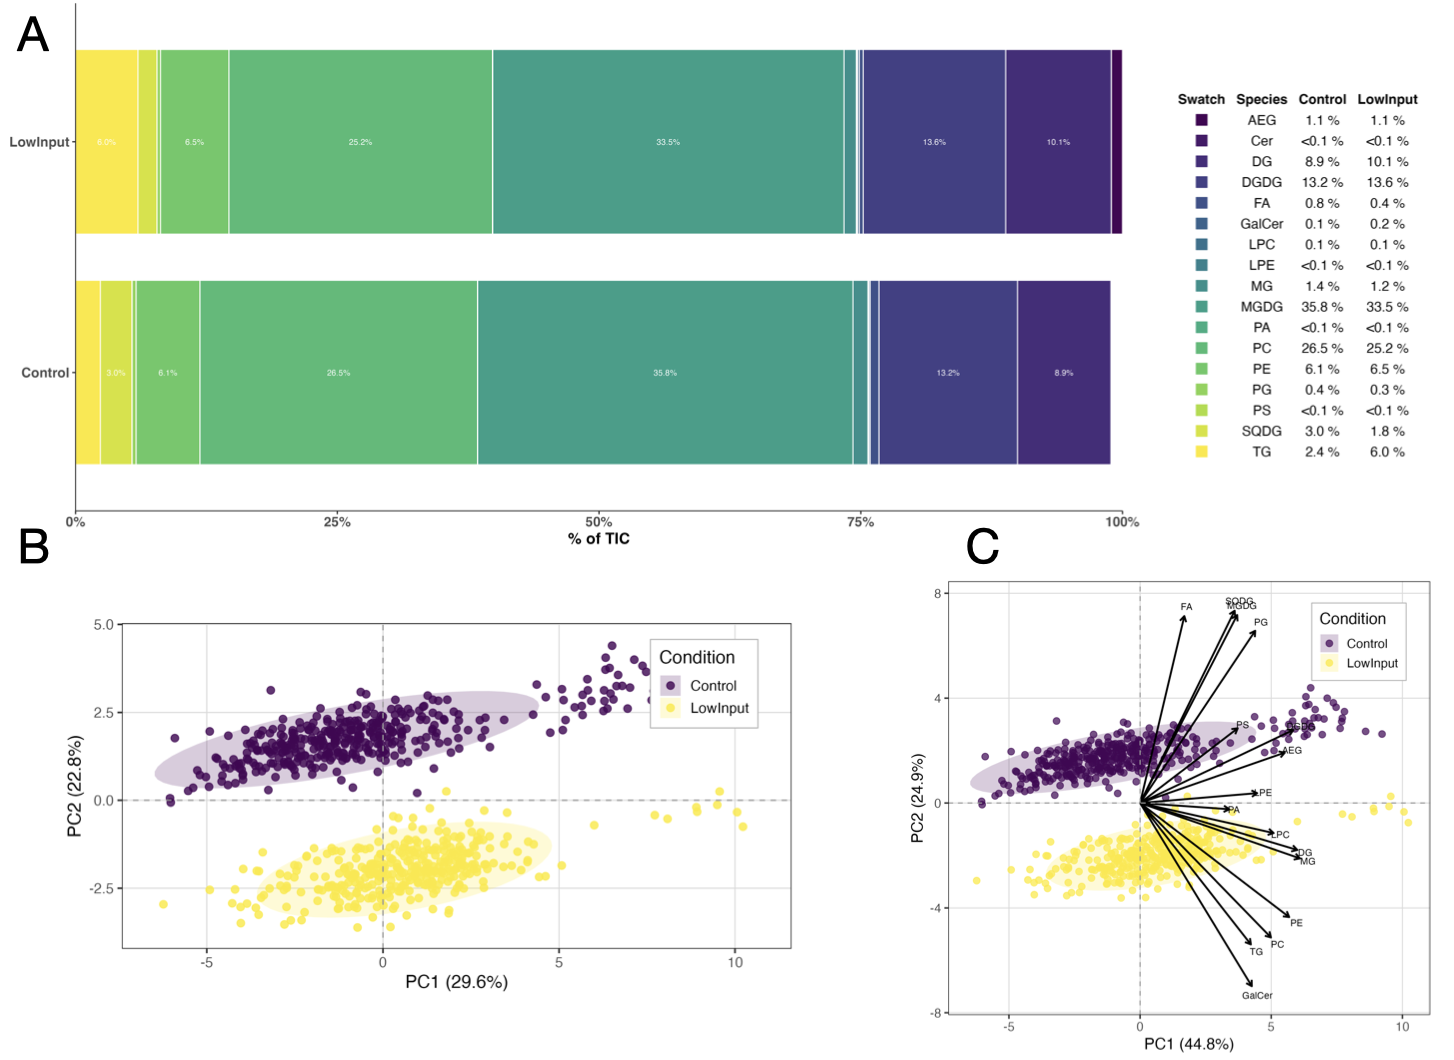
\includegraphics[width=\textwidth]{main/fig/Fig1.png}
  \caption{Overview of lipidomics results.  
    \textbf{A}: Mean lipid‐class composition (% of TIC) for Control vs.\ LowInput.  
    \textbf{B}: PCA of individual lipid species (PC1 = 29.6\%, PC2 = 22.8\%) with 95\% confidence ellipses.  
    \textbf{C}: PCA biplot showing class‐level loadings on PC1 (44.8\%) and PC2 (24.9\%).}
  \label{fig:Fig1_combined}
\end{figure}

\begin{figure}[htp]
  \centering

  %----------------------------------------------------
  %  (A) Full‐width: species‐level lipid composition
  %----------------------------------------------------
  \begin{subfigure}[t]{\textwidth}
    \centering
    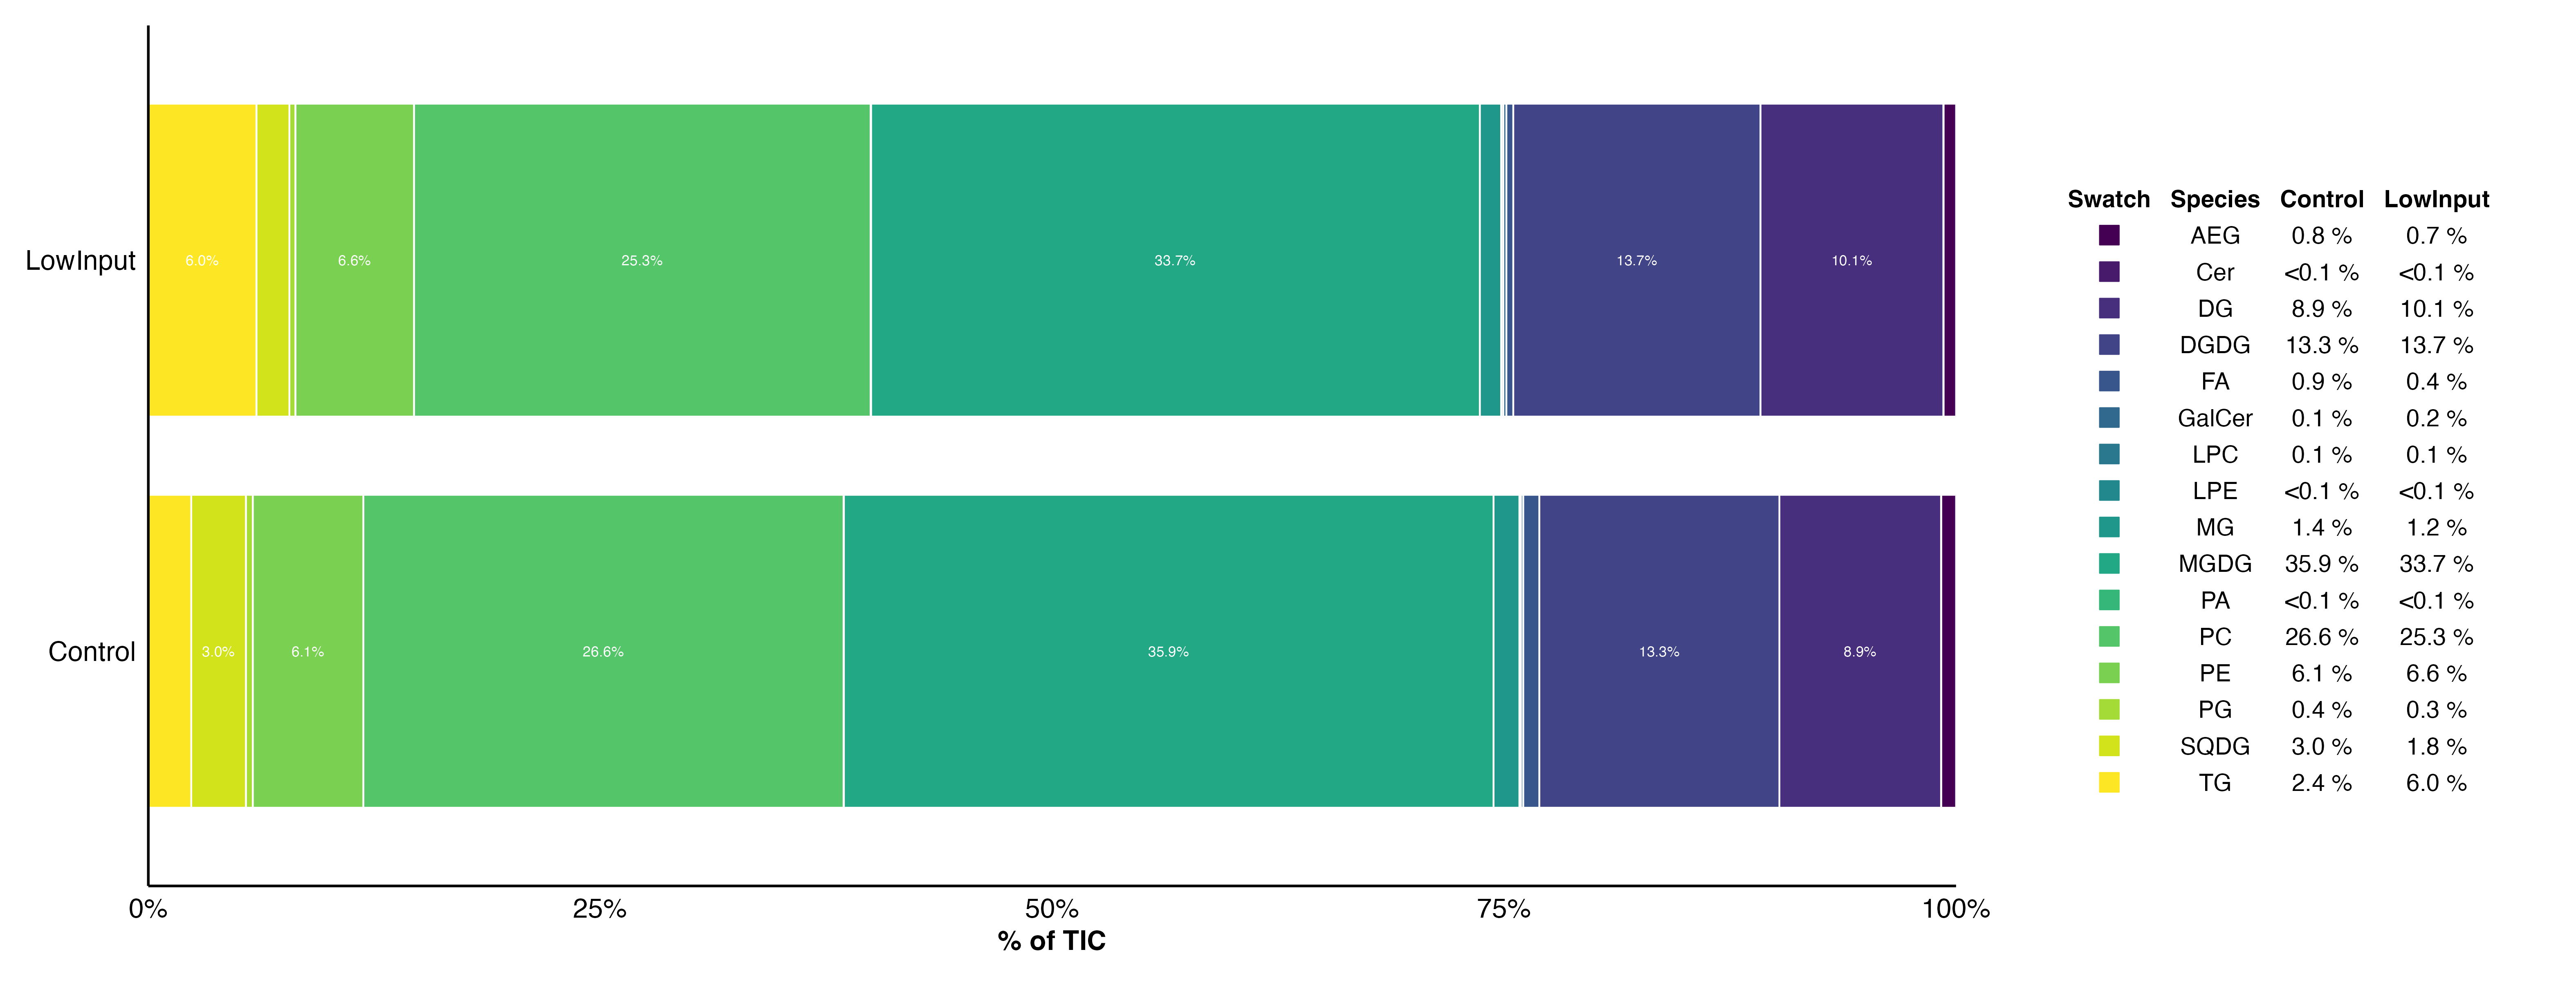
\includegraphics[width=\textwidth]{fig/main/Fig1a_lipid_species.png}
    \caption{Species‐level lipid composition (\% of TIC).}
    \label{fig:1A_lipid_species}
  \end{subfigure}

  \vspace{1em}

  %----------------------------------------------------
  %  (B) Full‐width: class‐level lipid composition
  %----------------------------------------------------
  \begin{subfigure}[t]{\textwidth}
    \centering
    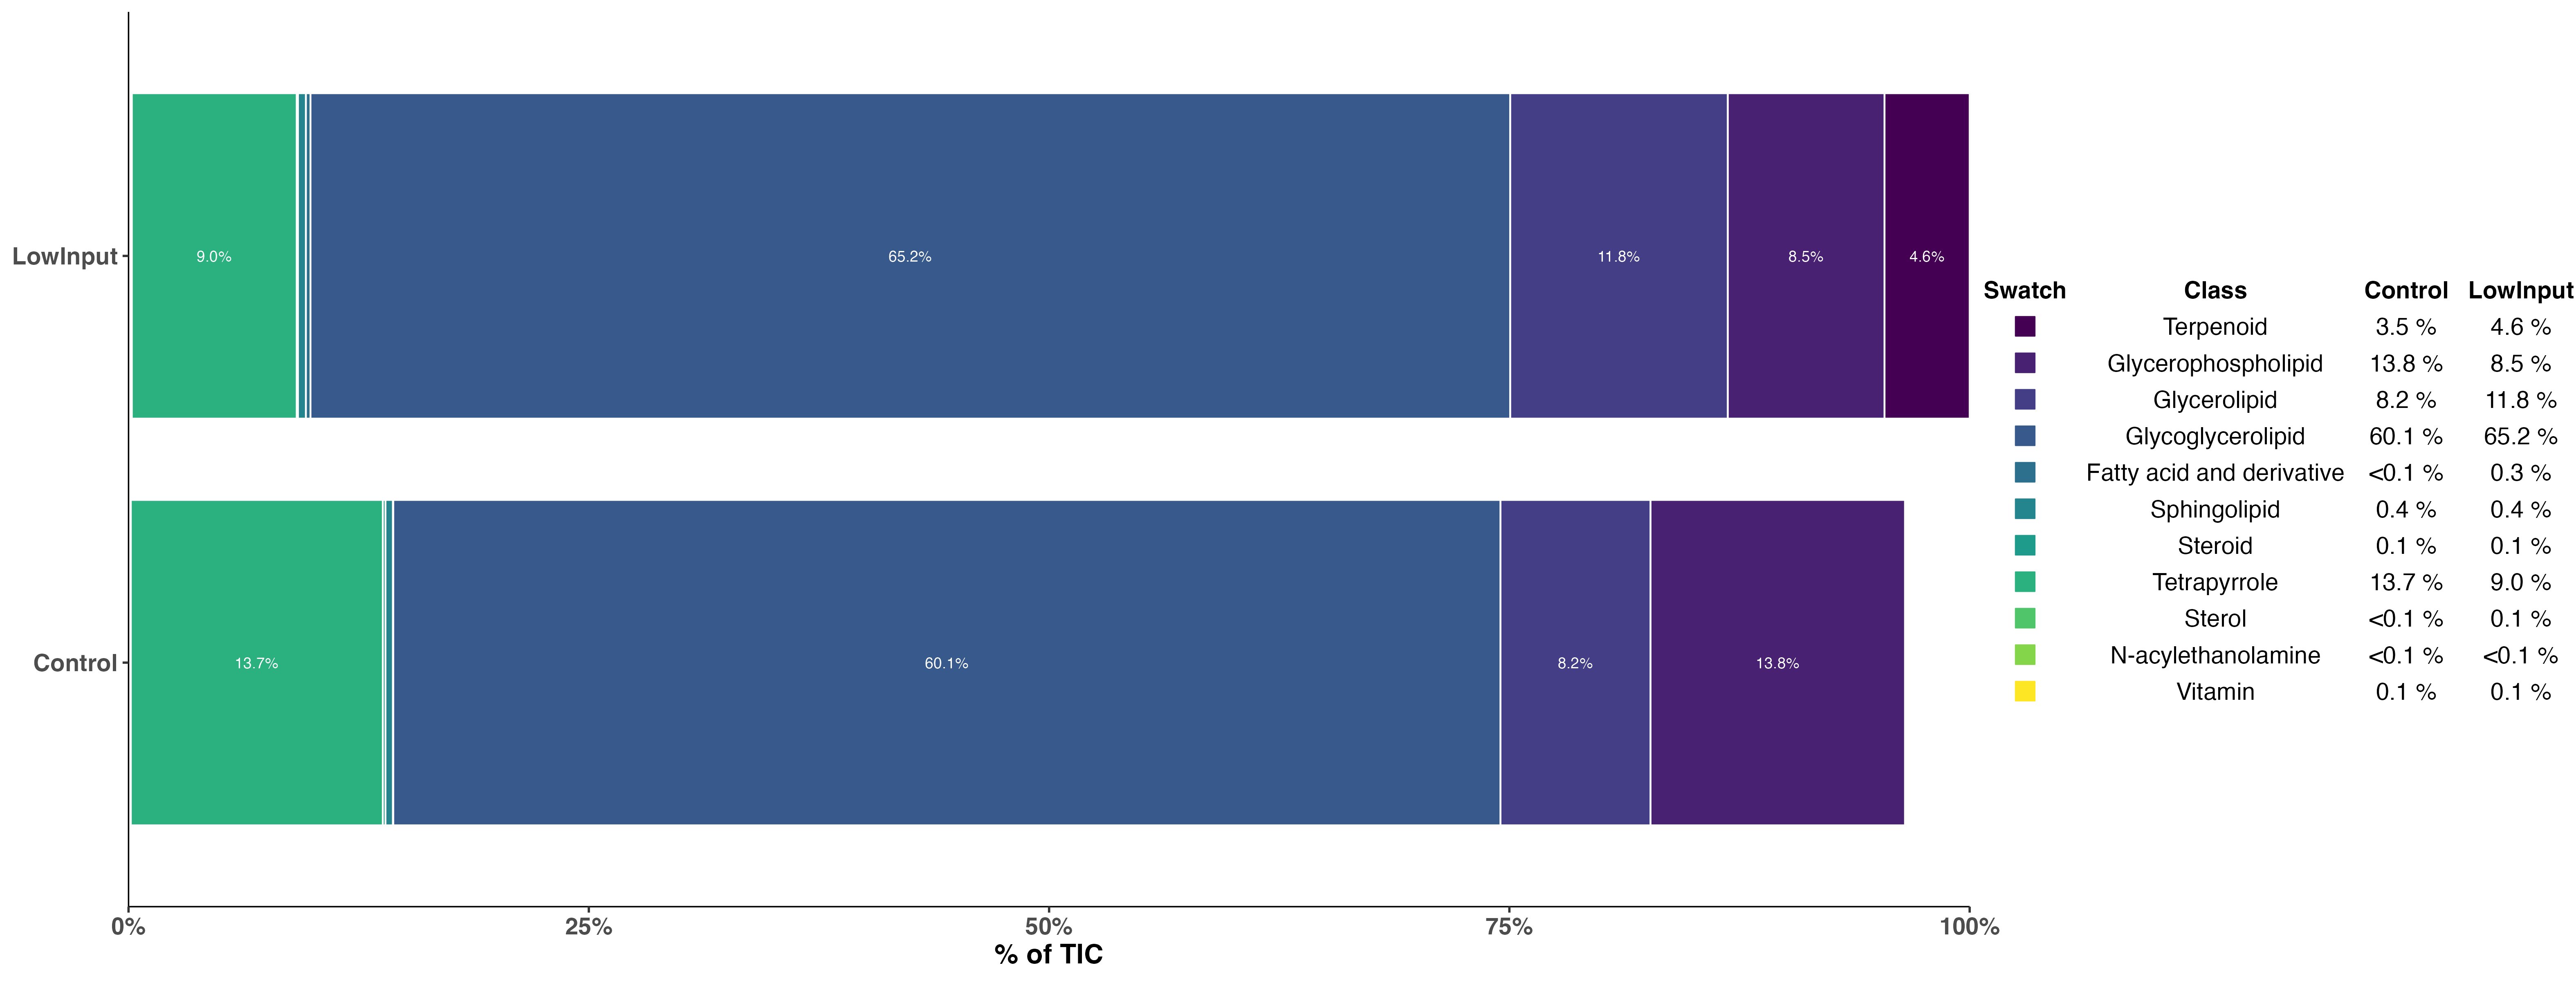
\includegraphics[width=\textwidth]{fig/main/Fig1b_lipid_class.png}
    \caption{Class‐level lipid composition (\% of TIC).}
    \label{fig:1B_lipid_class}
  \end{subfigure}

  \vspace{1em}

  %----------------------------------------------------
  %  (C) Bottom left: individual‐species PCA
  %----------------------------------------------------
  \begin{subfigure}[t]{0.48\textwidth}
    \centering
    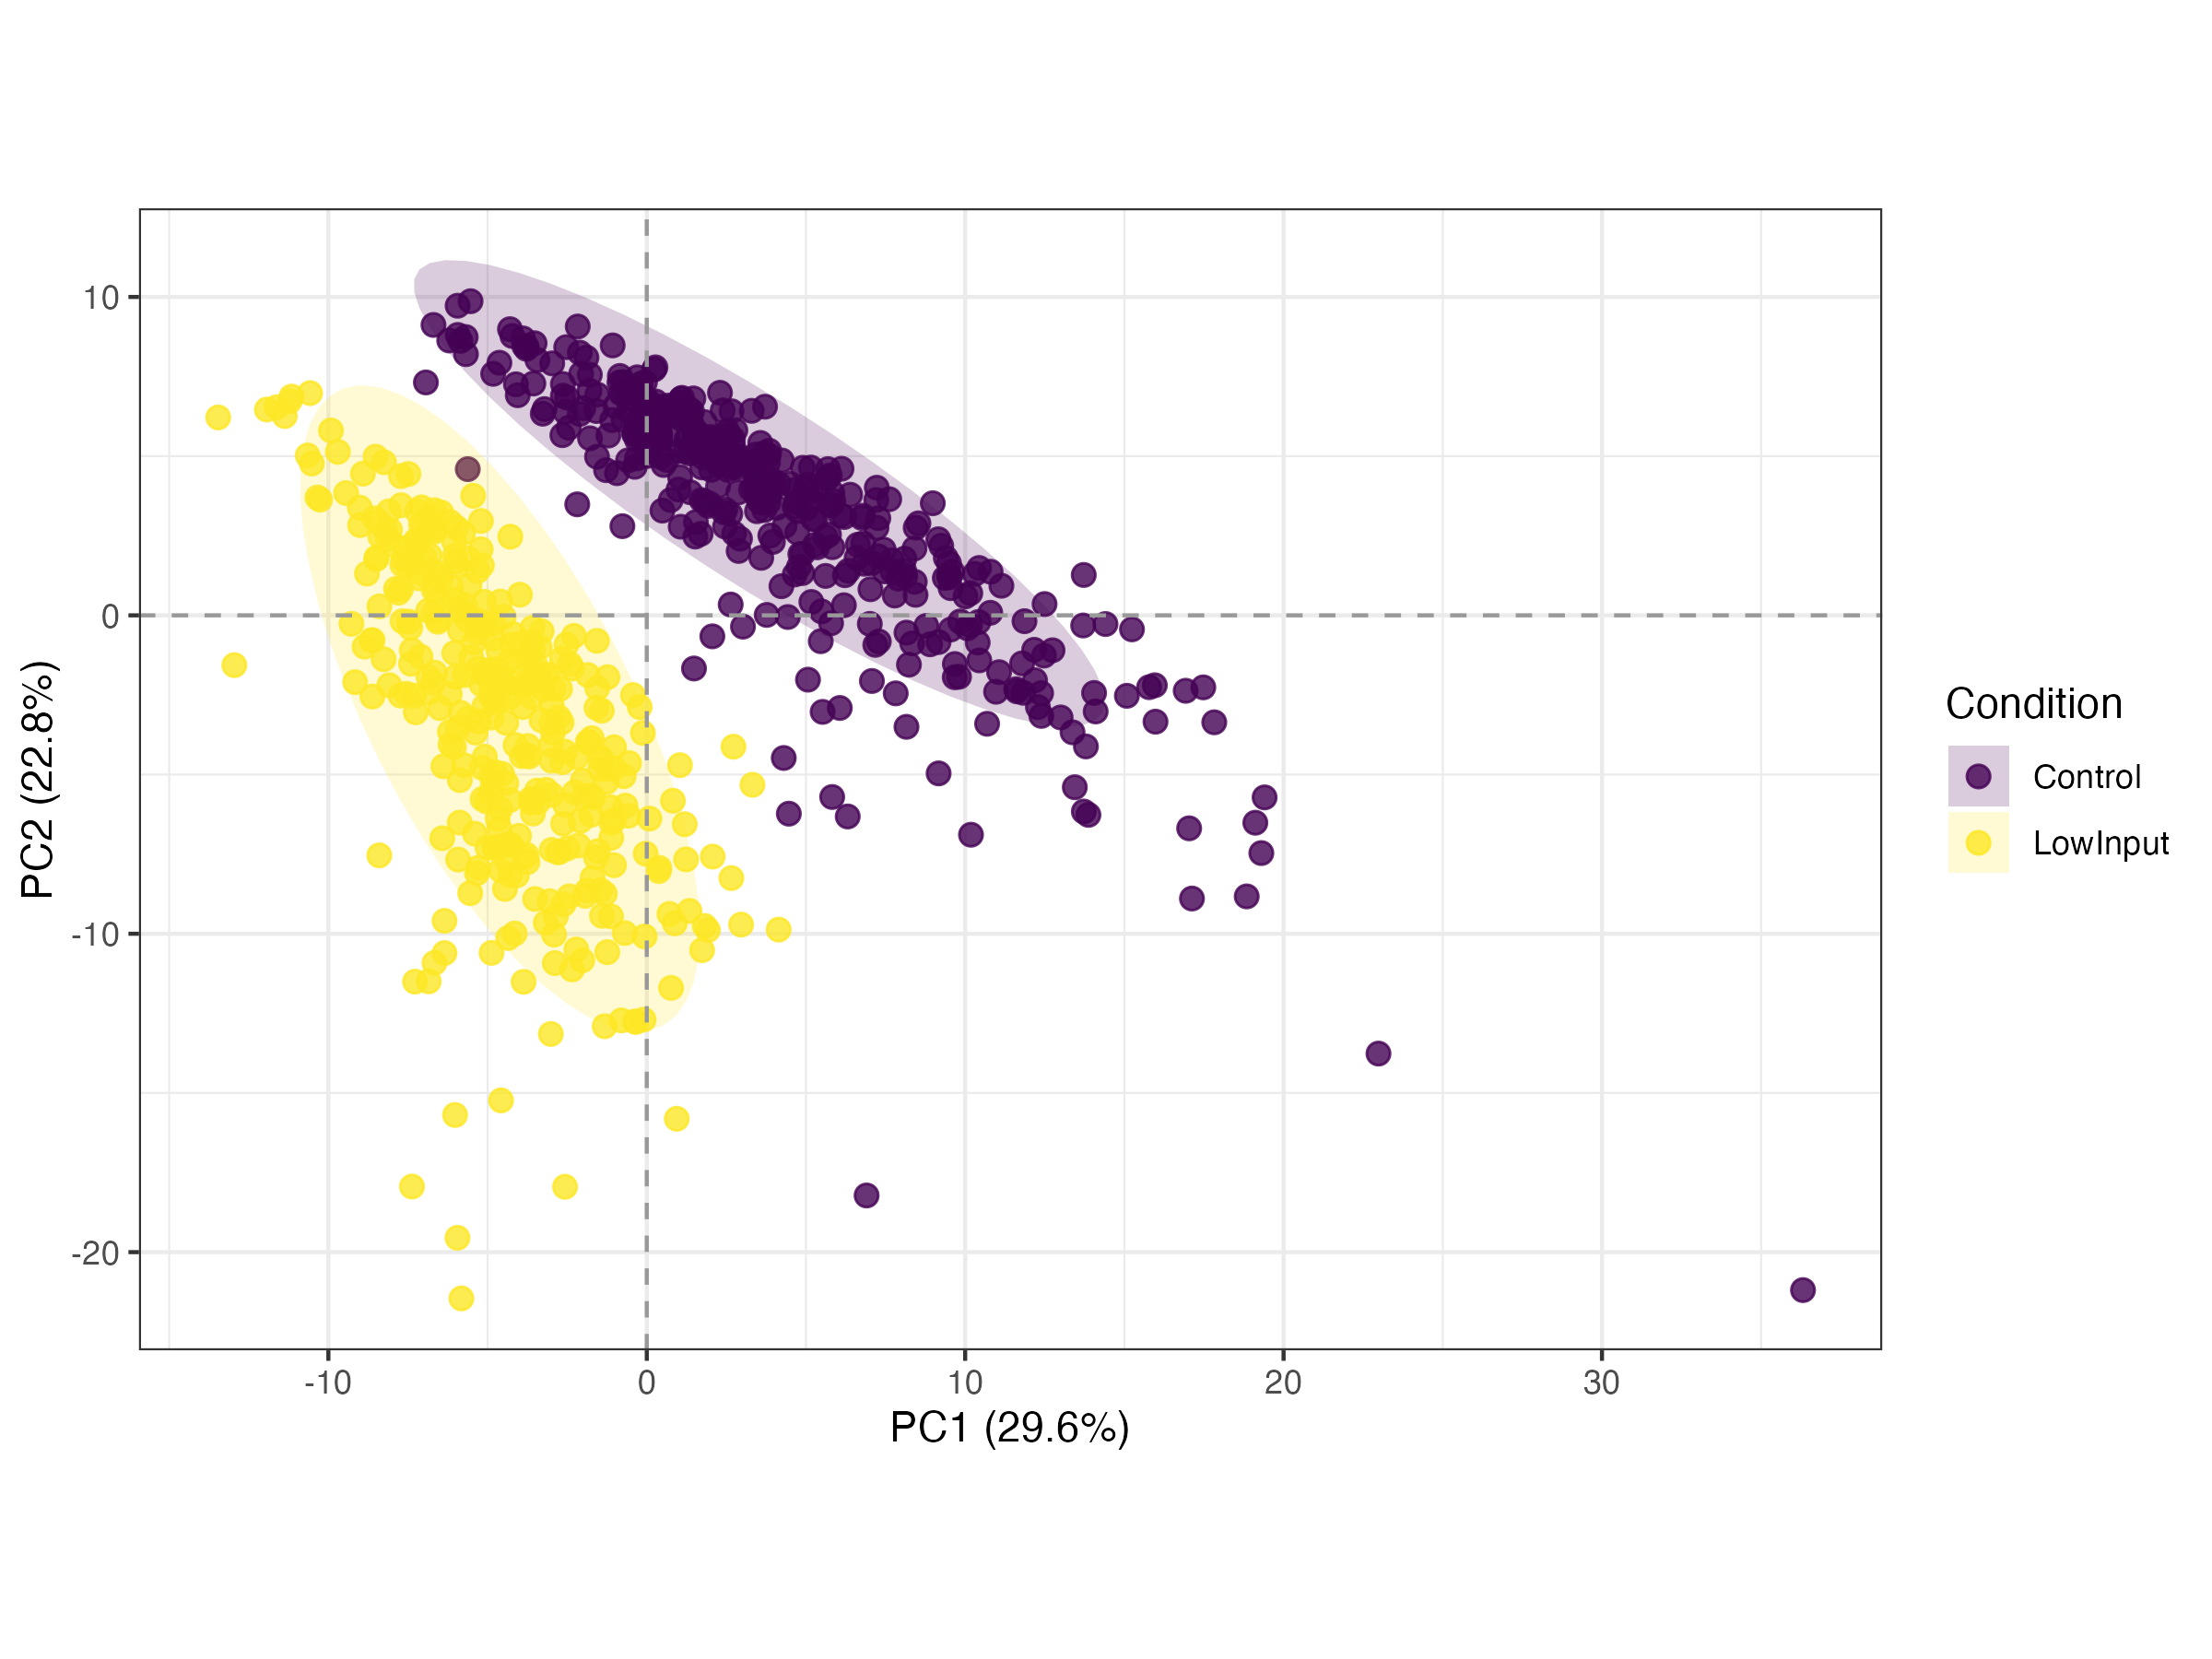
\includegraphics[width=\textwidth]{fig/main/Fig1c_individual_indv_lipid_PCA_plot.png}
    \caption{PCA biplot of individual lipid species (log‐TIC).}
    \label{fig:1C_species_pca}
  \end{subfigure}
  \hfill
  %----------------------------------------------------
  %  (D) Bottom right: summed‐class PCA biplot
  %----------------------------------------------------
  \begin{subfigure}[t]{0.48\textwidth}
    \centering
    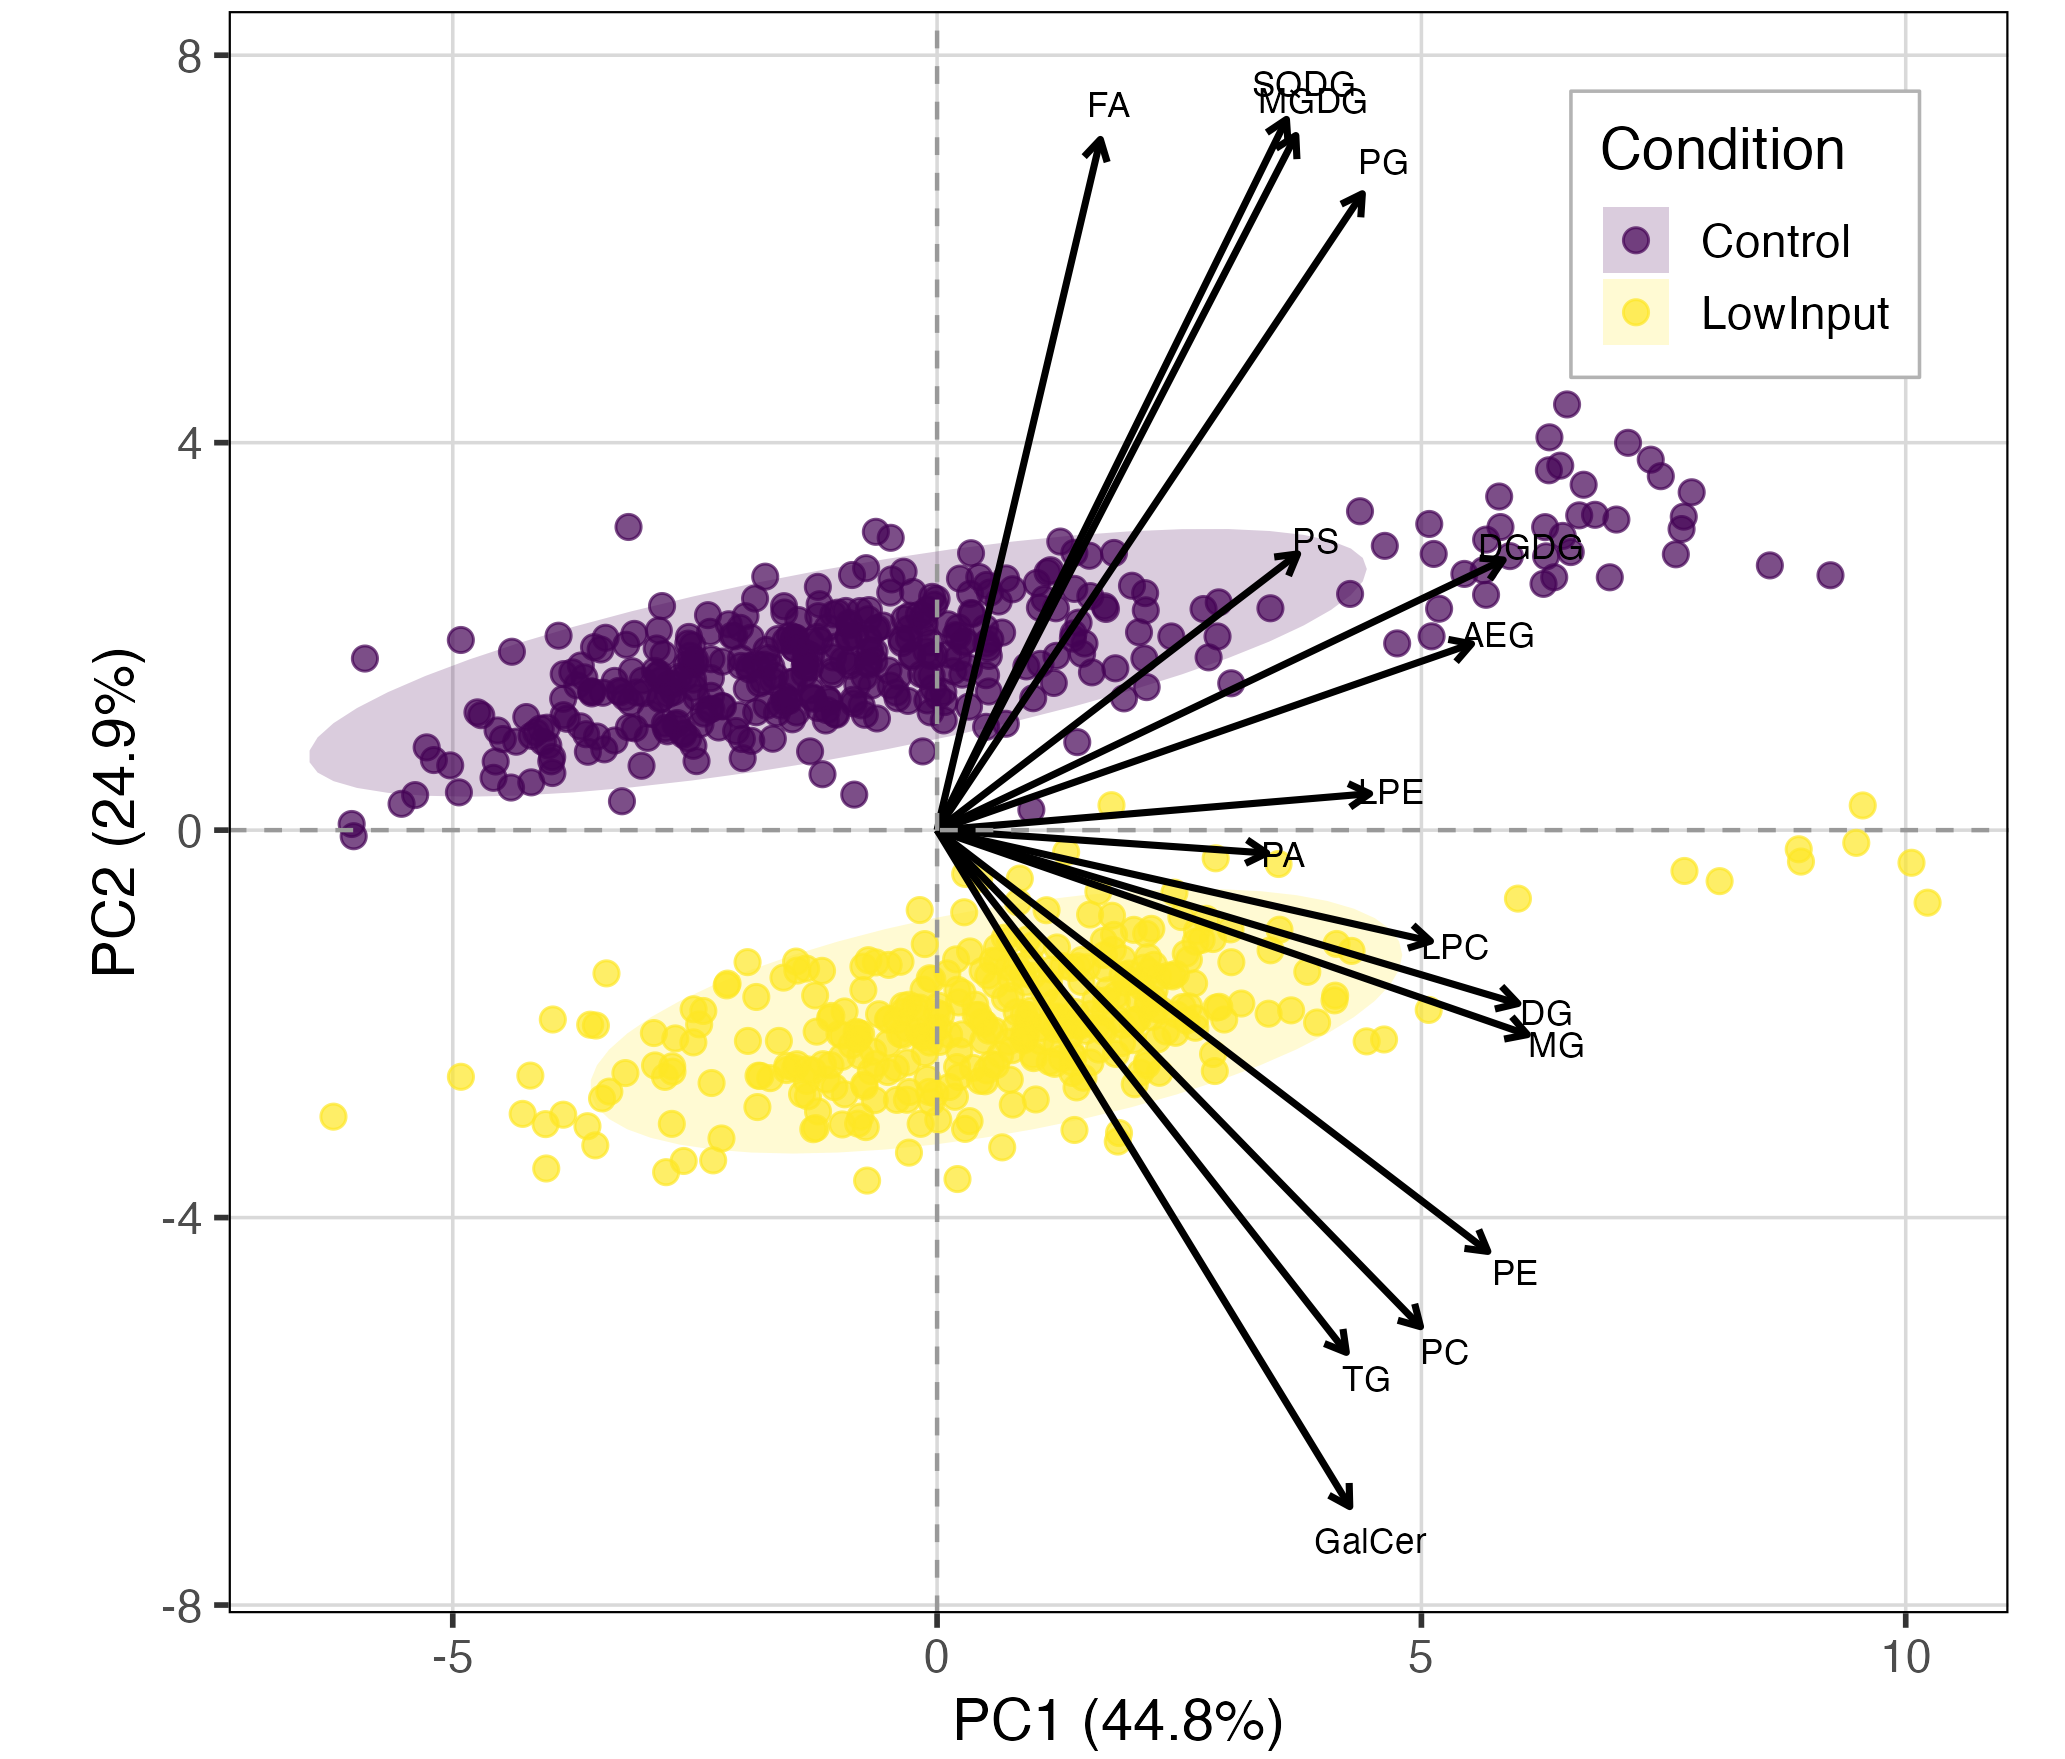
\includegraphics[width=\textwidth]{fig/main/Fig1d_summed_lipid_PCA_biplot.png}
    \caption{PCA biplot of summed lipid classes (with loadings).}
    \label{fig:1D_class_pca}
  \end{subfigure}

  \caption{%
    (A) Percent‐of‐TIC breakdown for individual lipid \emph{species}, averaged across all C (n = 384) and LI (n = 362) samples. Only species whose mean contribution ≥ 3 \% are labeled in‐bar.  
    (B) Percent‐of‐TIC breakdown for broader lipid \emph{classes}, averaged across the same sets of samples.  
    (C) PCA biplot of individual lipid species, with scores colored by condition and vectors showing species loadings. Each point represents a sample, projected based on the log-transformed relative abundance of all individual lipid molecules. Samples from the Control condition (purple) cluster in the upper-right quadrant, while those from the LowInput condition (yellow) shift toward the lower-left, indicating broad reprogramming of lipid composition under stress. The separation along PC1 (29.6%) and PC2 (22.8%) captures variance driven by both lipid abundance and diversity at the species level.
    (D) PCA biplot of summed lipid \emph{classes}, with sample scores and class‐ratio loadings.  
    In all panels, “Control” is shown in purple and “Low Input” in yellow.}
  \label{fig:lipid_main}
\end{figure}



\subsection*{Lipid Changes under LowInput (LI)}
The multi-year, multi-field experimental design introduced considerable environmental variability into the lipidomic profiles. Although spatial corrections (SpATS) and batch-effect normalization (SERRF) were employed, residual confounding factors necessitated a ratio-based analytical approach to compare the C and the LI conditions. Lipid class ratios, which demonstrate greater resilience to technical and environmental noise than absolute abundances, were prioritized to identify biologically conserved patterns of membrane adaptation. To mitigate these confounding effects, we concentrated on within-plant lipid class ratios, expected to be fairly consistent under a variety of cultivation environments, rather than absolute abundances. We aggregated individual molecular species into their respective lipid classes, computed all possible pairwise ratios on a linear scale, and subsequently applied OPLS-DA to identify the most discriminative ratios. The resulting scores plot (Fig. \ref{fig:OPLS}) demonstrated a robust separation of C versus LI samples, and the model exhibited exemplary performance metrics (R²Y = 0.99; Q²Y = 0.82) alongside a highly significant CV-ANOVA (p < 0.001) (Supp Figure, supp table). Hotelling’s T² analysis confirmed the absence of extreme outliers, and a 1,000-permutation test dismissed overfitting, indicating that our observations are unlikely attributable to chance. From the complete ratio set, 21 features surpassed a conservative VIP threshold of 1. Each of these high VIP ratios was then subjected to univariate testing (adjusted p < 0.05) and cross-verified against established pathways of membrane remodeling under cold and nutrient stress. The two-tier selection approach prioritizing statistical power and biological relevance yielded a defined set of lipid-class ratios (supp table) which may differentiate between C and LI.


\begin{figure}[htbp]
  \centering

  \begin{subfigure}[b]{0.28\textwidth}
    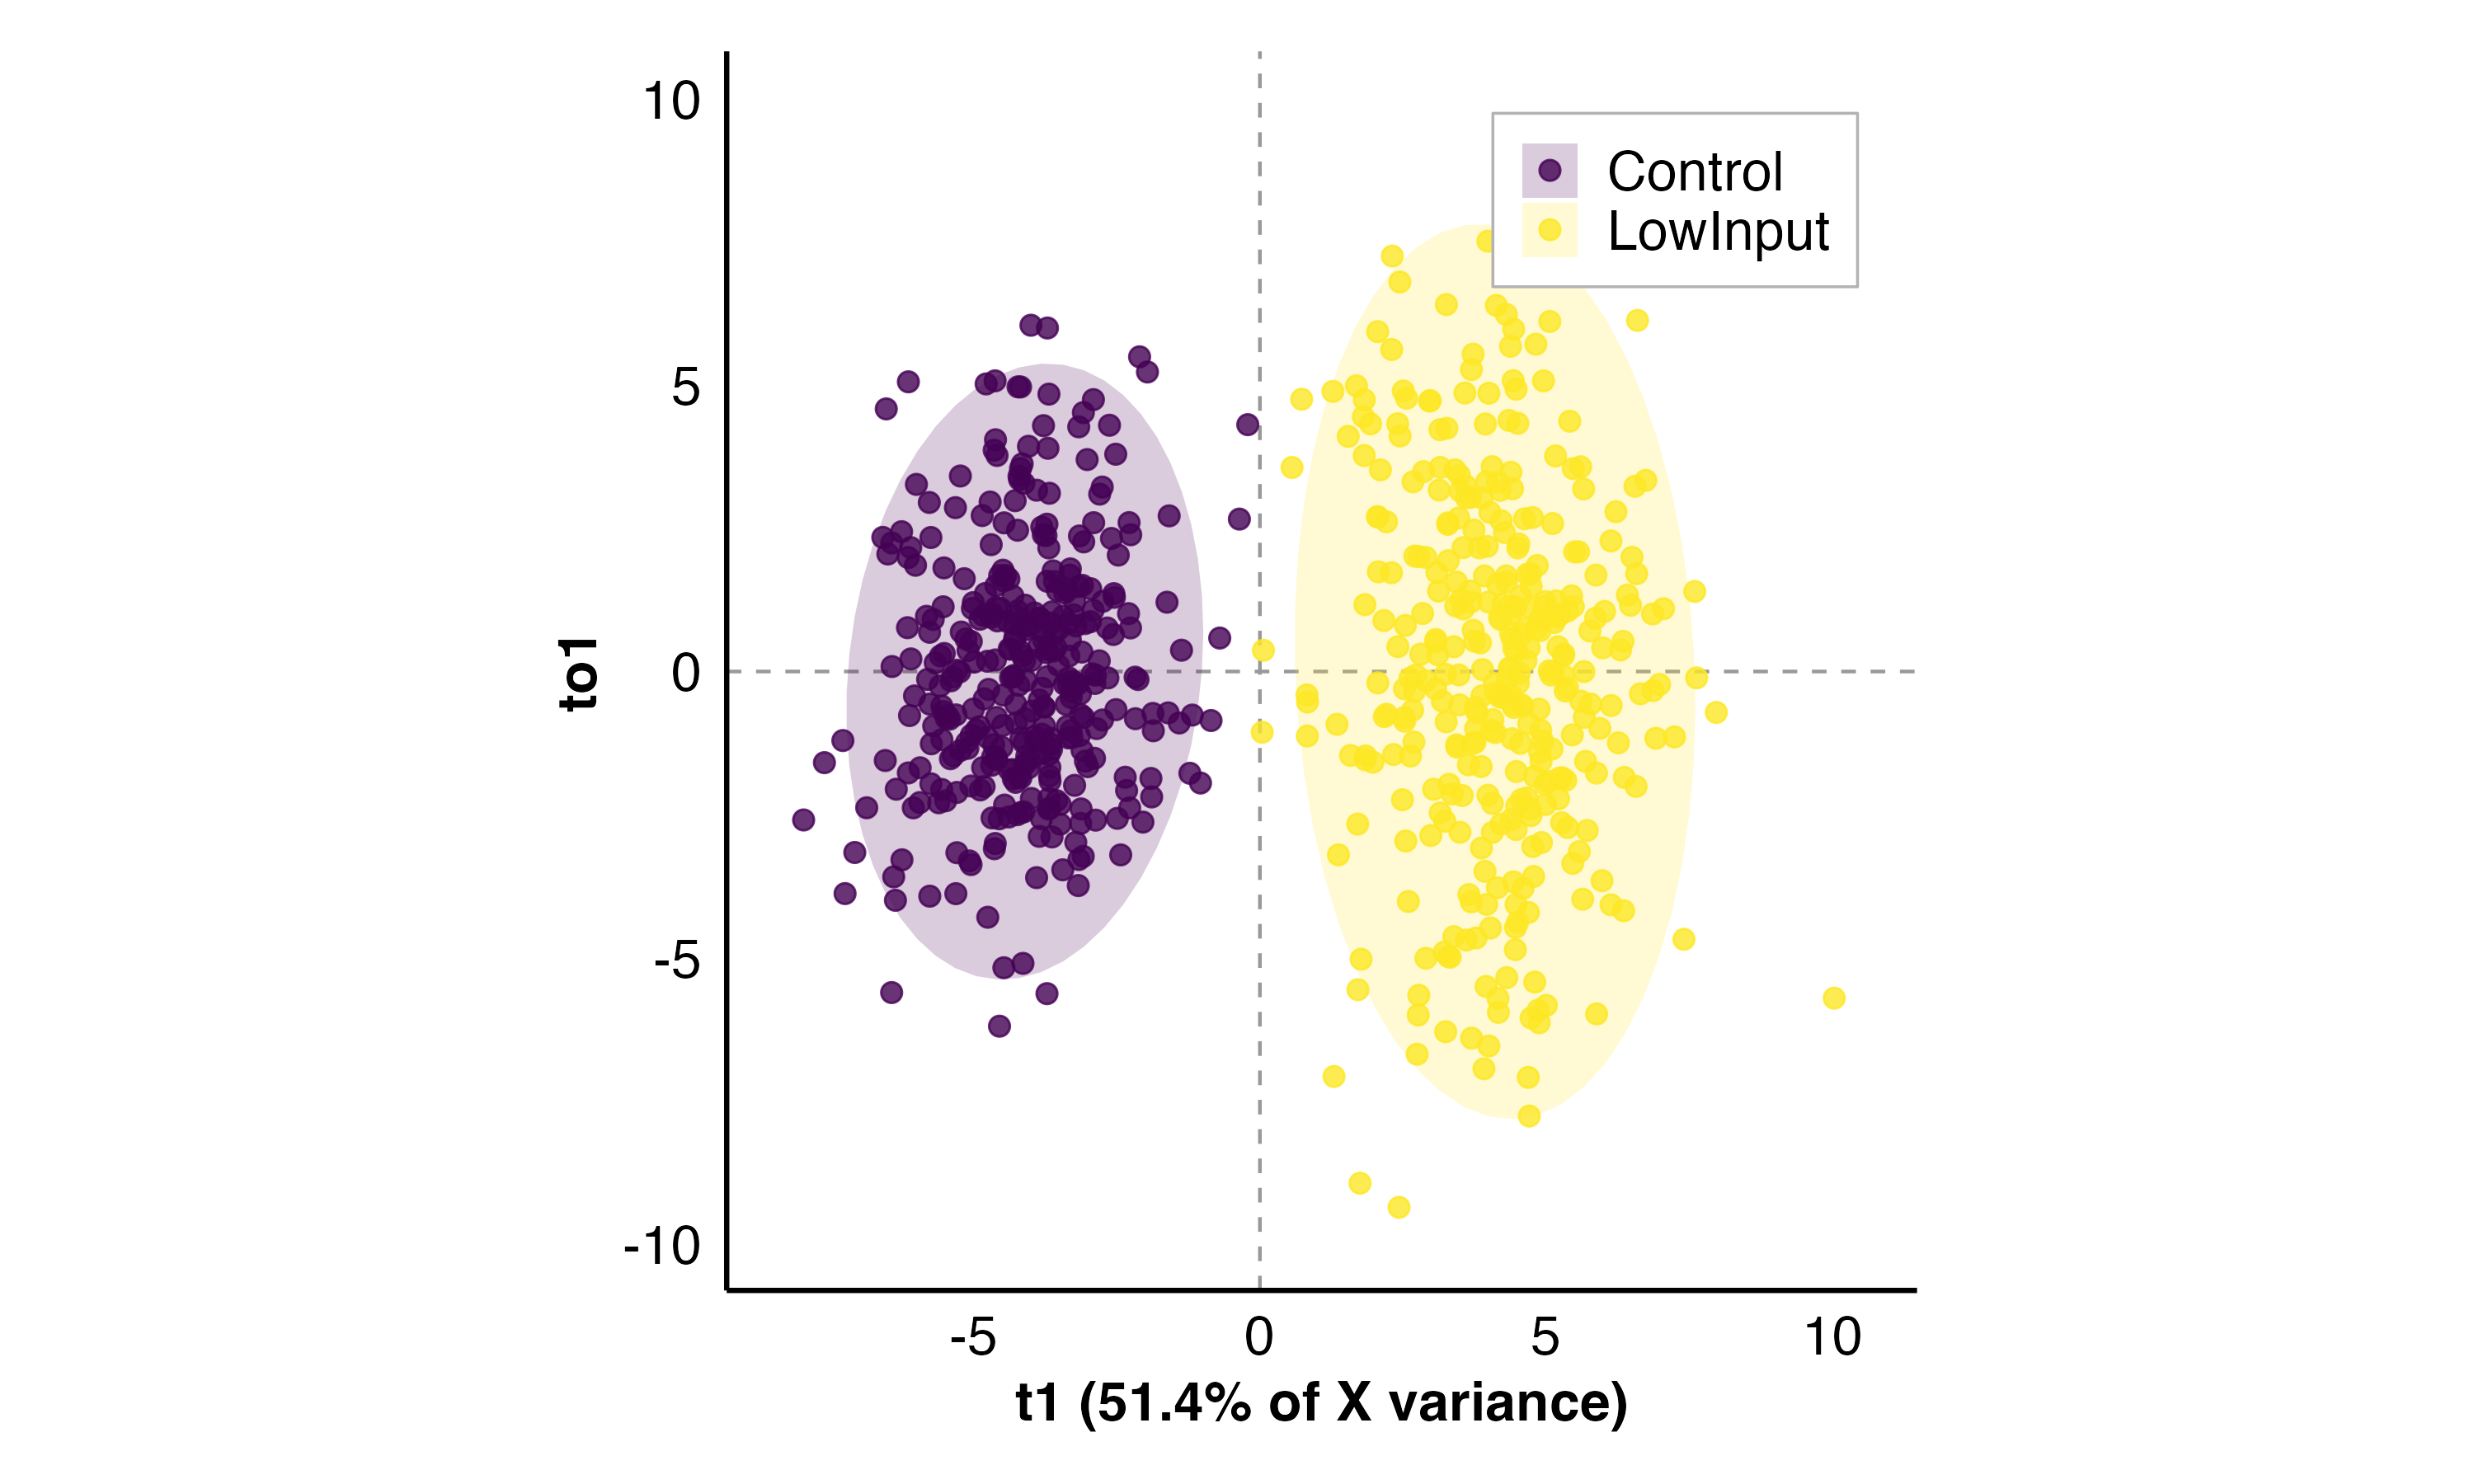
\includegraphics[width=\textwidth]{fig/main/Fig2a_OPLS_scores_plot.png}
    \caption{OPLS-DA score plot.} 
    \label{fig:opls_scores}
  \end{subfigure}
  \begin{subfigure}[b]{0.52\textwidth}
    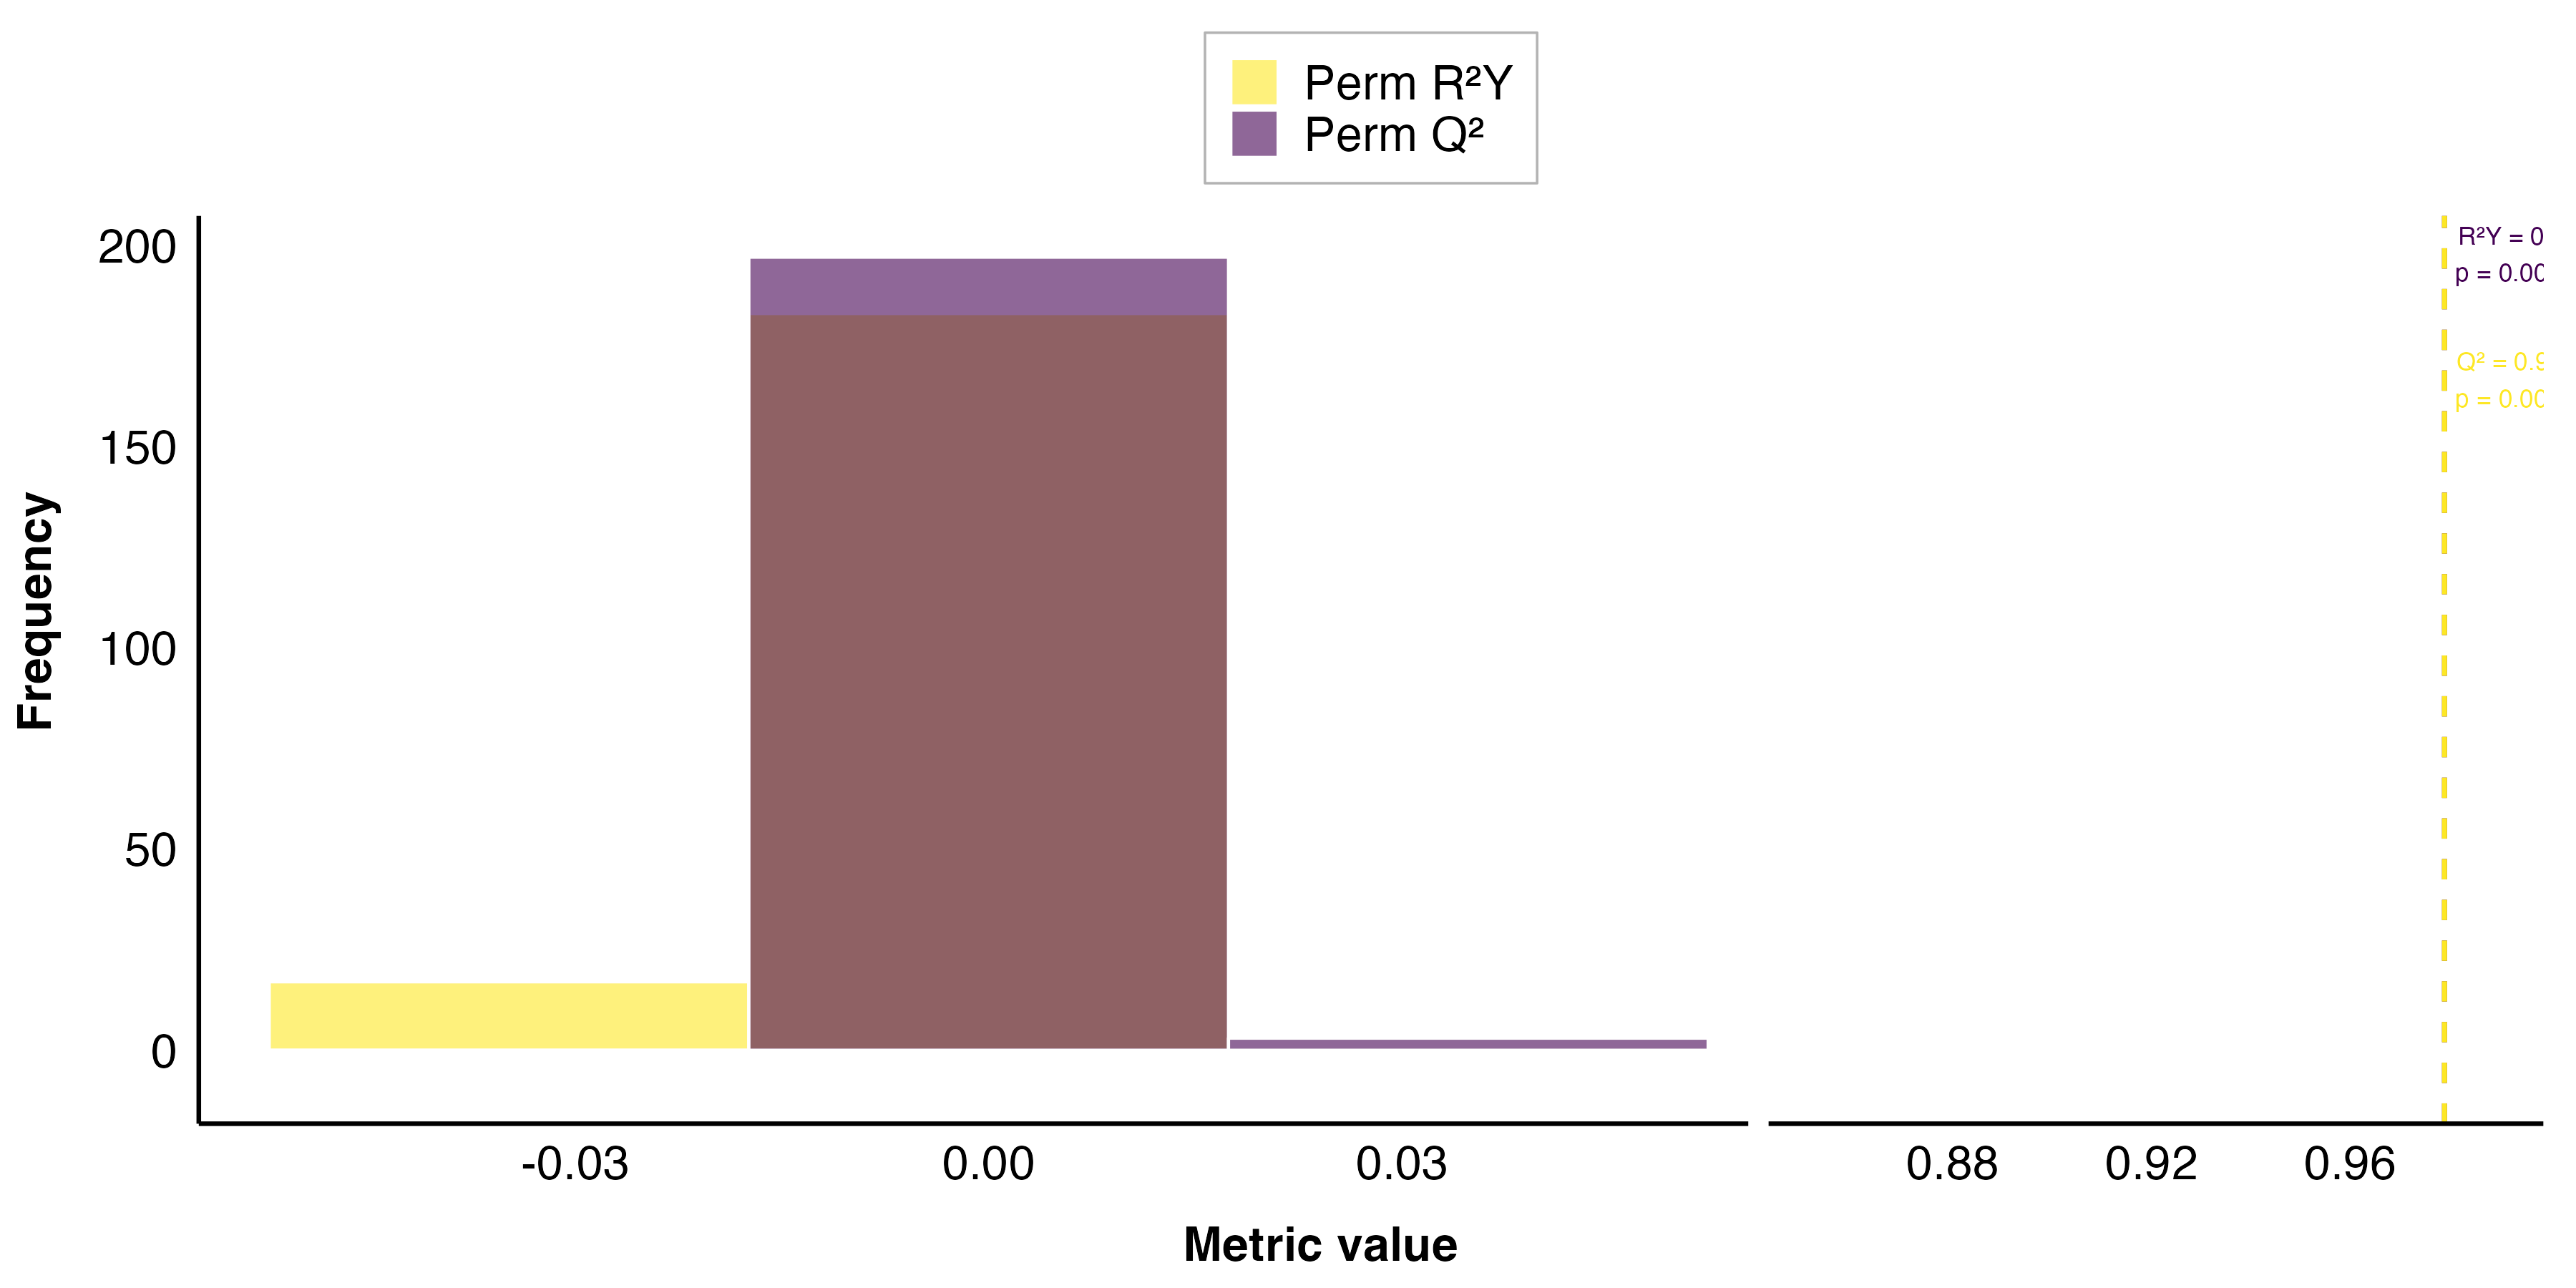
\includegraphics[width=\textwidth]{fig/main/Fig2b_OPLS_permutation_plot.png}
    \caption{Permutation validation. }
    \label{fig:opls_perm}
  \end{subfigure}

  \caption{Orthogonal projections to latent structures discriminant analysis (OPLS-DA) of lipidomic profiles. (a) Score plot showing clear separation between Control and LowInput groups along the predictive axis. Samples from the Control (purple) and LowInput (yellow) groups are projected onto the first predictive component ($t_1$, 51.4\% of $X$-variance) vs.\ the first orthogonal component ($\mathrm{to}_1$). Dashed grey lines mark zero; 95\% confidence ellipses highlight within-group clustering. (b) Permutation test demonstrating that both R²Y and Q² exceed all values obtained under random class assignments (200 permutations, $p=0.005$). Overlaid histograms of 200 permuted R²Y (yellow) and Q² (purple) show distributions under random label‐swaps; observed R²Y and Q² (dashed lines, $p=0.005$) lie well outside, confirming model significance. Arrow marks cumulative $X$-variance explained (R²X = 0.514).}
  \label{fig:OPLS}
\end{figure}




\begin{table}[!h]
\centering
\caption{\bf Most important lipid ratios based on OLSA-DA}
  \label{table:olsa}
\begin{tabular}{>{}l>{\raggedleft\arraybackslash}p{3cm}}
\toprule
\textbf{Lipid Ratio} & \textbf{VIP score}\\
\midrule
\textbf{\cellcolor{gray!10}{PE/SQDG}} & \cellcolor{gray!10}{1.62}\\
\textbf{MGDG/PC} & 1.61\\
\textbf{\cellcolor{gray!10}{PC/SQDG}} & \cellcolor{gray!10}{1.60}\\
\textbf{MGDG/PE} & 1.57\\
\textbf{\cellcolor{gray!10}{SQDG/TG}} & \cellcolor{gray!10}{1.50}\\
\addlinespace
\textbf{MG/SQDG} & 1.50\\
\textbf{\cellcolor{gray!10}{MGDG/TG}} & \cellcolor{gray!10}{1.49}\\
\textbf{DGDG/MGDG} & 1.49\\
\textbf{\cellcolor{gray!10}{DGDG/PC}} & \cellcolor{gray!10}{1.47}\\
\textbf{PC/PS} & 1.46\\
\addlinespace
\textbf{\cellcolor{gray!10}{MG/MGDG}} & \cellcolor{gray!10}{1.43}\\
\textbf{DGDG/PE} & 1.39\\
\textbf{\cellcolor{gray!10}{DGDG/SQDG}} & \cellcolor{gray!10}{1.32}\\
\textbf{DGDG/TG} & 1.24\\
\textbf{\cellcolor{gray!10}{LPE/PC}} & \cellcolor{gray!10}{1.23}\\
\addlinespace
\textbf{PE/PS} & 1.21\\
\textbf{\cellcolor{gray!10}{PS/TG}} & \cellcolor{gray!10}{1.15}\\
\textbf{MG/PC} & 1.15\\
\textbf{\cellcolor{gray!10}{LPC/MGDG}} & \cellcolor{gray!10}{1.13}\\
\textbf{LPC/SQDG} & 1.07\\
\addlinespace
\textbf{\cellcolor{gray!10}{LPE/TG}} & \cellcolor{gray!10}{1.07}\\
\textbf{LPE/PE} & 1.06\\
\textbf{\cellcolor{gray!10}{PC/PE}} & \cellcolor{gray!10}{1.05}\\
\textbf{LPC/PC} & 1.03\\
\bottomrule
\end{tabular}
\end{table}

\subsection*{1. Membrane Lipid Remodeling under LowInput (LI)}

\subsubsection*{1.1 Sulfolipid (SQDG) Collapse Under LI Stress Adaptation}

Under LI stress, SQDG is the lipid most susceptible to degradation, breaking down quickly prior to the remodeling of other membrane lipids (Fig.~\ref{fig:lipid_remodeling}\,“Sulfolipid Adjustments”).


% ------------------------------------------------------------------
%  Canonical behaviour of SQDG under single stresses
% ------------------------------------------------------------------
\begin{table}[!ht]
  \centering
  \caption{\bf Canonical responses of sulfoquinovosyldiacylglycerol (SQDG) under single abiotic stresses.}
  \label{table:SQDG_responses}
  \begin{tabular}{@{} l l c p{6cm} c @{}}
    \toprule
    \textbf{Class} 
      & \textbf{Stress} 
      & \textbf{Response} 
      & \textbf{Mechanism} 
      & \textbf{Ref.} \\
    \midrule
    \multirow{3}{*}{\textbf{SQDG}}
      & Low-P  & ↑ (strong induction)   
               & SQDG replaces anionic phospholipids (mainly PG) to maintain thylakoid surface charge while economizing phosphorus; up-regulation of SQD1/SQD2 diverts UDP-sulfoquinovose toward SQDG synthesis. 
               & [1] \\
      & Low-N  & ↓/≈ (variable)         
               & Nitrogen scarcity limits sulfate assimilation and UDP-sulfoquinovose production; DAG backbones are redirected to TAG or DGDG rather than SQDG. 
               & [2] \\
      & Cold   & ↑/≈ (species-dependent)
               & Cold acclimation often elevates SQDG for extra anionic buffering of PSII complexes; responses vary with species and sugar availability. 
               & [3] \\
    \bottomrule
  \end{tabular}
  \begin{flushleft}
    {\footnotesize Arrows denote relative change vs.\ control (↑ increase, ↓ decrease, ≈ no consistent change).}
  \end{flushleft}
\end{table}



\paragraph{Key Observations}
\begin{enumerate}
  \item \textbf{Preferential SQDG depletion relative to phospholipids: } \\ 
  Both SQDG/PC and SQDG/PG decrease significantly (LI $<$ Control, $p<0.001$), indicating that SQDG deteriorates more rapidly compared to the primary phospholipids in extraplastidial (\textit{PC}) and thylakoid (\textit{PG}) membranes.
  
  \item \textbf{SQDG loss outpaces DGDG: }\\
  SQDG decreases more significantly than DGDG ($p<0.001$), suggesting that DGDG is conserved to maintain bilayer stability. The potential high metabolic costs in terms of sulfur and energy, as well as its non-essential nature for short-term membrane integrity, make the breakdown of SQDG more prioritized. We define {SQDG\textsubscript{total}} as \(\bigl[\mathrm{SQDG}-\tfrac12(\mathrm{DGDG}+\mathrm{MGDG})\bigr]\). Furthermore, the total SQDG levels decline in LI ($p<0.001$), indicating an overall sulfolipid deficit. However, MGDG levels remain unchanged with respect to SQDG.
  
\end{enumerate}

\paragraph{Metabolic Interpretation and Physiological Significance}
\vspace{-0.5ex}
\begin{enumerate}
  \item \textbf{Sulfur salvage for stress defence.} \\ 
        SQDG breakdown yields sulfoquinovose, contributing sulfur for glutathione and other thiols that neutralize ROS during the initial phase of simultaneous cold and nutrient scarcity.
 % \item \textit{DG liberation fuels downstream pathways.}  
 %       DAG produced from SQDG hydrolysis explains the sharp rise in
 %       \(\mathrm{DG/SQDG}\) (Section 2); that DAG is later diverted to
 %       TAG rather than recycled into membranes.
  \item \textbf{Anionic‐lipid charge compensation.} \\
        The loss of SQDG is typically compensated by an increase in PG or DGDG during phosphorus deficiency. In this scenario, both the SQDG/Phospho and SQDG/Galacto ratios decrease, indicating that LI plants may tolerate a net decrease in anionic surface charge, which might be stabilized by the association with Ca\(^{2+}\) or Mg\(^{2+}\) in cold conditions.
\end{enumerate}



\subsubsection*{1.2 Galactolipid Dynamics}

 In LI treatment, galactolipid degradation becomes asymmetrical, with MGDG experiencing a greater depletion relative to DGDG. This imbalance signifies a tactical balance between energy efficiency and maintaining membrane integrity (see Fig.~\ref{fig:lipid_remodeling}, “Galactolipid Dynamics”):
% ------------------------------------------------------------------
%  Galactolipid behaviour (DGDG and MGDG)
% ------------------------------------------------------------------
\begin{table}[!ht]
  \centering
  \caption{\bf Canonical responses of the two major galactolipids (DGDG and MGDG) under single abiotic stresses.}
  \label{table:galactolipid_responses}
  \begin{tabularx}{\textwidth}{@{} l l p{3.5cm} X c @{}}
    \toprule
    \textbf{Class}
      & \textbf{Stress}
      & \textbf{Response}
      & \textbf{Mechanism}
      & \textbf{Ref.} \\
    \midrule
    \multirow{3}{*}{\textbf{Galactolipids}}
      & Low-P  
         & \begin{minipage}[t]{3.5cm}
             DGDG: ↑ replaces PC/PE;\\
             MGDG: ↑ replaces PC/PE
           \end{minipage}
         & DAG is redirected toward galactolipid synthesis, substituting for phospholipids under P limitation.
         & [1] \\[1ex]
      & Low-N  
         & \begin{minipage}[t]{3.5cm}
             DGDG: ↑/≈ (weak retention);\\
             MGDG: ↓
           \end{minipage}
         & Enhanced PC breakdown releases DAG that is partly channeled to DGDG, while MGDG declines as resources shift to storage lipids or other pathways.
         & [2] \\[1ex]
      & Cold   
         & \begin{minipage}[t]{3.5cm}
             DGDG: ↑ (bilayer stabilizer);\\
             MGDG: ↓ (converted or remodeled)
           \end{minipage}
         & Cold stress favors higher DGDG for maintaining bilayer stability; MGDG is remodeled or reduced to adjust membrane fluidity.
         & [3] \\
    \bottomrule
  \end{tabularx}
  \begin{flushleft}
    {\footnotesize Arrows denote relative changes vs.\ control (↑ increase, ↓ decrease, ≈ no significant change).}
  \end{flushleft}
\end{table}

\paragraph{Key Observations}
\begin{enumerate}
  \item \textbf{MGDG is the Primary Target of Degradation} \\
  The ratio \(\mathrm{MGDG/DGDG}\) decreases significantly (\(p<0.001\)), highlighting a more rapid depletion of MGDG compared to its bilayer-supporting counterpart, DGDG. This pattern may imply that stress-activated lipases, such as PLA1, preferentially hydrolyze MGDG. Additionally, the \(\mathrm{MGDG/PC}\) ratio and the composite measure \(\mathrm{MGDG}_{\mathrm{total}} = \mathrm{MGDG} - \tfrac12(\mathrm{DGDG}+\mathrm{SQDG})\) both show substantial reductions (\(p<0.001\)), indicating that MGDG is the primary lipid reserve to be depleted under LI stresses.
  
  \item \textbf{DGDG is Relatively Preserved but Outcompeted by Phospholipids} \\
  DGDG\_total which is \([\mathrm{DGDG} - \tfrac12(\mathrm{MGDG}+\mathrm{SQDG})]\) shows a significant increase (\(p<0.001\)), suggesting relative preservation (Fig. TIC). This retention of DGDG implies that membrane collapse is being avoided. Furthermore, both \(\mathrm{DGDG/PC}\) and \(\mathrm{DGDG/PE}\) decrease (\(p<0.001\)), indicating that while DGDG levels surpass those of MGDG, they are still being overtaken by phospholipid concentrations under stress. Interestingly, \(\mathrm{DGDG/PG}\) exhibits an increase (\(p<0.001\)), which indicates a shift in DGDG distribution that might stabilize photosystem II (PSII) complexes. The increase in PG$_{\text{retention}}$ underscores PG's active preservation relative to other phospholipids like PC and PE, aligning with its vital function in photosynthesis.
\end{enumerate}

\paragraph{Potential Physiological Implications}
\begin{enumerate}
  \item \textbf{Thylakoid Membrane Rigidification via Lipid Restructuring} \\
        The reduction in MGDG/DGDG suggests a shift from the non-bilayer arrangement of MGDG to the stable bilayer form of DGDG. This change likely serves to counteract fluidity alterations caused by cold and nutrient stress, thus increasing membrane rigidity. Furthermore, it could aid in preventing ion leakage during nutrient shortages, given that the bilayer structure of DGDG provides superior seal integrity compared to the hexagonal II phase inclination of MGDG.
  
  \item \textbf{Carbon channeling within galactolipid pathways.} \\ 
        The simultaneous reduction of MGDG\_total while total DGDG\_total levels are maintained or increased indicates a prioritization in resource allocation, where the breakdown of MGDG supports the continued synthesis of DGDG during LI stress conditions. This suggests that the activity of DGD1/2 synthase could remain active for a more extended period or resist low temperatures more effectively than MGD1/3 activities, possibly due to differences in enzyme stability and the requirement for a bilayer during stress. The degradation of MGDG may release carbon, which is then used for the ongoing synthesis of residual DGDG, mediated through recycled DG, and for the storage of TG (refer to the increase in TG/DG in Section 1.3).
  
  \item \textbf{Dual functionality of DGDG} \\ 
        The rise in DGDG/PG indicates that DGDG may partially substitute for PG’s anionic surface charge. %By shuffling anionic lipids—DGDG and PG—to the forefront, LI plants may also optimize binding sites for Ca\(^{2+}\) and Mg\(^{2+}\) ions. These cations bridge adjacent negatively charged headgroups, tightening bilayer packing and mitigating leakiness that would otherwise arise from headgroup depletion.
        PG is limited (↓ PG\_retention, \(p<0.001\)), and SQDG is inadequate in this capacity (↓ SQDG/PG, \(p<0.001\)), which underscores the unique dual role of DGDG as both a structural lipid and a charge buffer.
\end{enumerate}

%\paragraph{Proposed Regulatory Crossroads}
%\begin{itemize}
%  \item \textit{Differential enzyme sensitivities:}  
%        MGDG synthase (MGD1/2) activity may be more inhibited by combined Low-N/P/cold than DGDG synthases, leading to sharper MGDG loss.
%  \item \textit{Galactose precursor limitation:}  
%        Reduced UDP-galactose under nutrient/cold stress may throttle MGDG production more than DGDG, whose existing pools are preferentially maintained.
%\end{itemize}



\subsubsection*{1.3 Phospholipid Homeostasis}

Under LI stress, phospholipid pools are selectively reorganized (Fig.~\ref{fig:lipid_remodeling} “Phospholipid Homeostasis”):

\begin{table}[!ht]
  \centering
  \caption{\bf Canonical responses of PC, LPC and PG under single abiotic stresses.}
  \label{table:lipid_responses}
  \begin{tabular}{@{} l l c p{5.5cm} c @{}}
    \toprule
    \textbf{Class} 
      & \textbf{Stress} 
      & \textbf{Response} 
      & \textbf{Mechanism} 
      & \textbf{Ref.} \\
    \midrule
    \multirow{3}{*}{\textbf{PC}} 
      & Low-P  & ↓ (major P donor)      
               & Phospholipase-mediated PC hydrolysis releases choline and phosphate; DAG backbone is redirected to DGDG or TAG synthesis. 
               & [1] \\
      & Low-N  & ↓ (N-source)          
               & Choline head-group catabolism supplies nitrogen; DAG is channeled into TAG accumulation. 
               & [2] \\
      & Cold   & ↑/≈ (species‐dependent) 
               & Increased PC unsaturation preserves bilayer fluidity; net PC often maintained or slightly elevated. 
               & [3] \\
    \addlinespace
    \multirow{3}{*}{\textbf{LPC}} 
      & Low-P  & ↑ (lipase product)    
               & PLA$_2$ activity rises to liberate phosphate; LPC is subsequently exported or re-acylated. 
               & [4] \\
      & Low-N  & ↓/≈                   
               & Reduced phospholipase activity conserves N-rich head-groups; DAG is preferred for storage rather than LPC re-acylation. 
               & [5] \\
      & Cold   & ↑                      
               & Rapid acyl-editing cycle (LPC ↔ PC) supports insertion of unsaturated acyl chains for cold acclimation. 
               & [6] \\
    \addlinespace
    \multirow{3}{*}{\textbf{PG}} 
      & Low-P  & ↓/≈                   
               & Partially substituted by SQDG to conserve phosphorus, yet basal PG is retained for PSII function. 
               & [7] \\
      & Low-N  & ≈/↓                   
               & PG contains no nitrogen; levels remain largely stable with only minor decline if DAG is diverted to TAG. 
               & [8] \\
      & Cold   & ↑ (thylakoid stabilizer)
               & Extra PG supports PSII dimer stability and optimizes electron transport at low temperature. 
               & [9] \\
    \bottomrule
  \end{tabular}
  \begin{flushleft}
    {\footnotesize Arrows denote relative change vs.\ control (↑ increase, ↓ decrease, ≈ no consistent change).}
  \end{flushleft}
\end{table}

\begin{enumerate}
  \item \textbf{PC/PE Asymmetry Suggests Membrane Rigidification} \\
  The substantial rise in PC/PE (\(p<0.001\)) suggests a favored preservation or production of PCs rather than PEs. The methylated headgroup of PC contributes to enhancing bilayer stability under conditions of low temperature and limited nutrients, whereas PE, with its smaller headgroup and tendency toward non-bilayer formations, is comparatively reduced.
  
  \item \textbf{PC/PG Increase Reflects Photosynthetic Trade-offs} \\
  PG retention is specific to plastids (refer to ↑DGDG/PG, section 1.2), though its overall quantity diminishes relative to PC. This reduction might aid in maintaining non-plastidic membrane structure as PG is depleted. Additionally, the increase in PC could potentially counterbalance the loss of thylakoid lipids (as indicated by ↓ MGDG\_retention and ↓ SQDG\_retention, section 1.2, Galactolipids, Dynamics).
  
  \item \textbf{PG\_retention Decline Highlights Metabolic Cost} \\
  The retention of PG (\(\mathrm{PG} - \tfrac12(\mathrm{PC} + \mathrm{PE})\)) decreases significantly (\(p<0.001\)), indicating that although PG is actively preserved for thylakoid functionality, its overall pool diminishes when compared to total phospholipids. The formation of PG depends on CDP-DAG and glycerol-3P, processes that are energy-demanding and may be reallocated under stress conditions.
  
  \item \textbf{NonP\_Phosphorus Decline Signals P-Limitation} \\
  The metric for non-P lipids, represented by \(\bigl[(\mathrm{MGDG}+\mathrm{DGDG})-(\mathrm{PC}+\mathrm{PE})\bigr]\), shows a significant decrease (\(p<0.001\)). This indicates that galactolipids and sulfolipids are less prominent compared to phospholipids, despite being non-phosphorus lipids. This observation deviates from the expected behavior during classic P starvation. In contrast to P limitation alone, the combined stress does not lead to an increase in the DGDG/PC ratio (↓ DGDG/PC), implying that the constraints from cold and nitrogen conditions overshadow the typical lipid shifts associated with P deficiency.

\end{enumerate}

\paragraph{Physiological Implications}
\begin{enumerate}
  \item \textbf{Bilayer fluidity prioritization.}  \\
        Elevated PC/PE ratio indicates that plants treated with LI alter headgroup composition to keep membrane viscosity optimal in cold, low N/P environments.
  
  \item \textbf{Selective anionic lipid allocation.}  \\
        While there is an overall reduction in PG, the rise in PC/PG ratios and the dynamics of PG retention suggest a dual approach: most of the PG is forfeited, yet a crucial portion is conserved within photosynthetic membranes.> 
  
  \item \textbf{Failure of classic galactolipid replacement.}  \\
        The decrease in the non-P:P metric indicates that, unlike straightforward P-starvation, LI plants are unable to replace phospholipids with galacto- and sulfolipids, probably due to simultaneous cold, N and P restrictions.
\end{enumerate}

%\paragraph{Proposed Regulatory Crossroads}
%\begin{itemize}
%  \item \textit{PC/PE Balance Control Point:}  
%        There might be a preferential activation of the Kennedy pathway's PC branch (via CTP:phosphocholine cytidylyltransferase). Similarly a potential PE N-methyltransferase (PEAMT) up regulation. Selective retention of PC through suprressed phospholipase D (PLD) activity. This makes is contrast with the classic P-starvation response. 
%  \item \textit{PG Biosynthesis Bottleneck:}  
%        Declining PG retention despite photosynthetic needs indicates that CDP-DAG:glycerol-3-phosphate phosphatidyltransferase (PGP1) becomes rate-limited. Possible competition for glycerol-3-phosphate (diverted to glycolysis/TAG). There could also be a possible cold-induced enzyme instability in PG synthesis pathway. 
%  \item \textit{Galactolipid Substitution Blockade:}  
%        Failed non-P lipid substitution (NonP\_Phosphorus) reveals interesting results. Due to N-limitation, UDP-galactose pool might be depleted which are required for the galactolipids. MGD/DGD synthase that produces the galactolipids might be inhibited due to the cold stress as well. We see that the carbon flux is redirected towards the PC/TAG rather than the galactolipids.      
%\end{itemize}


\subsection*{2. Lipid Turnover and Signaling under LowInput (LI)}

LI stress profoundly alters DG dynamics and lysophospholipid metabolism, reflecting a shift from membrane maintenance toward emergency carbon redeployment (Fig.~\ref{fig:lipid_remodeling} “Lipid Turnover and Signaling”):

\subsubsection*{2.1 Diacylglycerol (DG) Flux Hub}
\begin{enumerate}
  \item \textbf{DG Flux Hub Reveals Metabolic Bottlenecks} \\
  The significant rise in both DG/DGDG and DG/MGDG (\(p<0.001\)) suggests a quick buildup or insufficient recycling of DG as galactolipids break down, which implies that DAG kinase activity may be inhibited within plastids.
  
  \item \textbf{Cytosolic DG Starvation} \\
  DG/PC and DG/PE show a notable reduction (\(p<0.001\)), indicating that this DG pool is not reintroduced into the principal phospholipids. In the same vein, DG\_Phospho \(\bigl[\mathrm{DG} - \tfrac12(\mathrm{PC}+\mathrm{PE})\bigr]\) also decreases (\(p<0.001\)). This implies that the Kennedy pathway circumvents free DG and utilizes CDP-DAG directly. It also reveals PLD inhibition (↓lysoPLs), which curtails phospholipid-derived DG.
  
  \item \textbf{SQDG-DG Coupling}
  Rising levels of DG/SQDG (\(p<0.001\)) align with the degradation of SQDG providing DG backbones, which initially accumulate temporarily, before being channeled elsewhere (Section 1.1).
\end{enumerate}

% ------------------------------------------------------------------
%  Canonical behaviour of diacylglycerol (DG) under single stresses
% ------------------------------------------------------------------
\begin{table}[!ht]
  \centering
  \caption{\bf Canonical responses of diacylglycerol (DG) under single abiotic stresses.}
  \label{table:DG_responses}
  \begin{tabularx}{\textwidth}{@{} l l p{3.5cm} X c @{}}
    \toprule
    \textbf{Class}
      & \textbf{Stress}
      & \textbf{Response}
      & \textbf{Mechanism}
      & \textbf{Ref.} \\
    \midrule
    \multirow{3}{*}{\textbf{DG}}
      & Low-P  
         & \begin{minipage}[t]{3.5cm}
             DG: ↑ (phospholipase product)
           \end{minipage}
         & PC/PE hydrolysis liberates DAG backbones that serve as precursors for DGDG or TAG when phosphate is scarce.
         & [1] \\[1ex]
      & Low-N  
         & \begin{minipage}[t]{3.5cm}
             DG: ↑↑ (strong accumulation)
           \end{minipage}
         & Choline head-group catabolism from PC generates surplus DAG; limited acyl-CoA supply slows reconversion, so DAG pools rise.
         & [2] \\[1ex]
      & Cold   
         & \begin{minipage}[t]{3.5cm}
             DG: ↑ / transient pulse
           \end{minipage}
         & Rapid phospholipase A/C activity produces DAG for acyl remodelling; a transient DAG spike precedes re-acylation into cold-adapted PC or TAG.
         & [3] \\
    \bottomrule
  \end{tabularx}
  \begin{flushleft}
    {\footnotesize Arrows denote relative change vs.\ control (↑ increase, ↑↑ strong increase, ↓ decrease, ≈ no consistent change).  Replace reference placeholders with appropriate citations.}
  \end{flushleft}
\end{table}


\paragraph{Physiological Implications}
\begin{enumerate}
  \item \textbf{DG as a transient carbon hub.}  \\
        The increase in DG (DG/DGDG, DG/MGDG, DG/SQDG), along with its absence from phospholipid pools (DG/PC, DG/PE, DG\_phospho), indicates that DG is being redirected towards storage lipids such as TG, emphasizing the formation of energy reserves over the urgent need for membrane repair.
\end{enumerate}


 % \item \textit{Shift toward storage lipid synthesis.}  
 %       Accumulated DG likely feeds into triacylglycerol synthesis (see Section 3), reflecting a strategic rerouting of carbon from membrane maintenance to energy storage during prolonged stress.

\subsubsection*{2.2 Lysophospholipid Remodeling}
\begin{enumerate}
  \item \textbf{Global Lyso-phospholipid Reduction} \\
  LPC/PC, LPE/PE, and Lyso\_activity \(\bigl[(\mathrm{LPC} + \mathrm{LPE}) - (\mathrm{PC} + \mathrm{PE})\bigr]\) exhibit a significant reduction (\(p<0.001\)), suggesting either inhibited phospholipase activity or accelerated removal of lysophospholipids to preserve membrane integrity, indicating an overall reduction in phospholipid turnover. This suggests inhibition of phospholipase A2 (PLA2) under stress conditions. Furthermore, it coincides with ↓DG/Phospho, indicating reduced phospholipid turnover.

\end{enumerate}

\paragraph{Physiological Implications}
\begin{enumerate}
  \item \textit{Conservation of membrane integrity.}  
        The notable reduction in lysophospholipids and overall Lyso\_activity suggests a decreased phospholipase activity for deacylation, thus safeguarding current bilayers from further damage due to simultaneous cold and nutrient scarcity.
\end{enumerate}

% ------------------------------------------------------------------
%  Combined canonical behaviour of LPC, LPE and their ratios 
% ------------------------------------------------------------------
\begin{table}[!ht]
  \begin{adjustwidth}{-2.25in}{0in}  % adjust as needed for your page
    \centering
    \caption{\bf Canonical responses of lysophospholipids (LPC, LPE) and their ratios under single abiotic stresses.}
    \label{table:lyso_combined}
    %
    % Part A: LPC & LPE pools
    %
    \subcaption*{A) Lysophospholipid Pools}
    \vspace{-0.5em}
    \begin{tabularx}{\textwidth}{@{} l l p{3.5cm} X c @{}}
      \toprule
      \textbf{Class} & \textbf{Stress} & \textbf{Response} & \textbf{Mechanism} & \textbf{Ref.} \\
      \midrule
      \multirow{3}{*}{\textbf{LPC}}
        & Low-P  & ↑ (lipase product) & PLA\textsubscript{2} activity rises to liberate phosphate; LPC is exported or rapidly reacylated. & [1] \\
        & Low-N  & ↓ / ≈              & Lipase activity suppressed to conserve N-rich PC; DAG backbone preferentially routed to TAG, not LPC. & [2] \\
        & Cold   & ↑ (acyl editing)   & Active PC ↔ LPC cycle inserts unsaturated acyl chains for cold acclimation. & [3] \\
      \addlinespace
      \multirow{3}{*}{\textbf{LPE}}
        & Low-P  & ↑ (lipase product) & PE hydrolysis releases phosphate; transient LPE spikes before re-acylation. & [4] \\
        & Low-N  & ↓ / ≈              & LPE formation limited by N scarcity; DAG diverted to storage lipids. & [5] \\
        & Cold   & ↑ (remodelling)    & PE ↔ LPE exchange supports insertion of unsaturated fatty acids. & [6] \\
      \bottomrule
    \end{tabularx}

    \vspace{1em}

    %
    % Part B: LPC/PC and LPE/PE ratios
    %
    \subcaption*{B) Lysophospholipid / Phospholipid Ratios}
    \vspace{-0.5em}
    \begin{tabularx}{\textwidth}{@{} l l p{3cm} X c @{}}
      \toprule
      \textbf{Ratio} & \textbf{Stress} & \textbf{Response} & \textbf{Interpretation} & \textbf{Ref.} \\
      \midrule
      \multirow{3}{*}{\(\tfrac{\mathrm{LPC}}{\mathrm{PC}}\)}
        & Low-P  & ↑            & Diagnostic of enhanced PLA\textsubscript{2}-mediated P scavenging. & [7] \\
        & Low-N  & ↓            & Choline head-group salvage limits LPC formation. & [8] \\
        & Cold   & ↑ (transient)& Rapid acyl editing before re-acylation restores PC pool. & [9] \\
      \addlinespace
      \multirow{3}{*}{\(\tfrac{\mathrm{LPE}}{\mathrm{PE}}\)}
        & Low-P  & ↑            & Reflects PE hydrolysis under P limitation. & [10] \\
        & Low-N  & ↓ / ≈        & Lipase repression conserves PE; LPE remains low or unchanged. & [11] \\
        & Cold   & ↑            & Enzymatic LPEAT-driven exchange introduces unsaturated chains. & [12] \\
      \bottomrule
    \end{tabularx}

    \vspace{0.5em}
    \begin{flushleft}
      {\footnotesize Arrows denote relative change vs.\ control (↑ increase, ↓ decrease, ≈ no consistent change).  
      Replace reference placeholders with appropriate citations.}
    \end{flushleft}
  \end{adjustwidth}
\end{table}



\subsection*{3. Carbon Sink and Allocation}

Under LI stress, carbon is progressively redirected from structural membranes into neutral storage lipids (Fig.~\ref{fig:lipid_remodeling} "Carbon Sink and Allocation"):

% ------------------------------------------------------------------
%  Canonical behaviour of triacylglycerol (TG) under single stresses
% ------------------------------------------------------------------
\begin{table}[!ht]
  \begin{adjustwidth}{-2.25in}{0in}  % Remove if the table already fits
    \centering
    \caption{\bf Canonical responses of triacylglycerol (TG) under single abiotic stresses.}
    \label{table:TG_responses}
    \begin{tabularx}{\textwidth}{@{} l l l X c @{}}
      \toprule
      \textbf{Class} & \textbf{Stress} & \textbf{Response} & \textbf{Mechanism (summary)} & \textbf{Ref.} \\
      \midrule
      \multirow{3}{*}{\textbf{TG}}
        & Low-P & ↑ / ≈ (species dependent) &
          Moderate TAG rise when excess DAG is *not* entirely channelled to DGDG;  
          P-starved cells deposit surplus carbon in TAG while conserving phospholipid-derived P. & [1] \\[0.4em]
        & Low-N & ↑↑ (strong induction) &
          Nitrogen shortage limits protein synthesis and sinks carbon into storage lipids;  
          PC breakdown supplies DAG that is rapidly acylated to TAG via DGAT/PDAT pathways. & [2] \\[0.4em]
        & Cold  & ↑ (energy buffer) &
          Cold stress slows growth and promotes TAG accumulation as a temporary carbon/energy reservoir;  
          unsaturated TAG species also scavenge free fatty acids released during membrane remodelling. & [3] \\
      \bottomrule
    \end{tabularx}
    \begin{flushleft}
      {\footnotesize Arrows denote relative change vs.\ control (↑ increase, ↓ decrease, ≈ no consistent change).  
      Replace reference placeholders with appropriate citations.}
    \end{flushleft}
  \end{adjustwidth}
\end{table}




\subsubsection*{3.1 Storage Lipid Reallocation}
\begin{enumerate}
  \item \textbf{Compartmentalized Carbon Redirection to Storage} \\
  TG/DG significantly increases (\(p<0.001\)), indicating a potent transformation of DG into TG, likely facilitated by DGAT enzymes external to membrane lipid recycling. Additionally, the TG/Galacto ratio \(\bigl[\mathrm{TG} - \tfrac{1}{2}(\mathrm{MGDG}+\mathrm{DGDG})\bigr]\) rises (\(p<0.001\)), suggesting that DG is directed away from galactolipids in chloroplasts to be stored. The DG\_to\_Gala value \(\bigl[\mathrm{DG} - \tfrac{1}{2}(\mathrm{MGDG}+\mathrm{DGDG})\bigr]\) also grows (\(p<0.001\)), reflecting an accumulation of DG relative to galactolipid pathways.

  \item \textbf{Storage over Phospholipid Maintenance}
  TG/Phospho \(\bigl[\mathrm{TG} - \tfrac{1}{2}(\mathrm{PC}+\mathrm{PE})\bigr]\) is significantly increased (\(p<0.001\)), suggesting that TG synthesis for storage is more prominent than the upkeep of membrane phospholipids, even with PC/PE conservation.
  
\end{enumerate}


\subsubsection*{3.2 Metabolic Trade-offs}
\begin{enumerate}
  \item \textbf{Photosynthetic Machinery Sacrificed for Storage} \\
  The metric \(\bigl[\tfrac{1}{2}(\mathrm{TG} + \mathrm{DG}) - \tfrac{1}{2}(\mathrm{MGDG} + \mathrm{DGDG})\bigr]\) shows a substantial increase (\(p<0.001\)), suggesting that carbon is being redirected from not only structural membranes but also from photosynthetic galactolipid reserves to TG storage.
  
  \item \textbf{Storage\_vs\_Membrane} \\
    \(\bigl[\tfrac{1}{2}(\mathrm{TG} + \mathrm{DG}) \;-\; \tfrac{1}{2}(\mathrm{PC} + \mathrm{PE})\bigr]\) rises significantly(\(p<0.001\)), showing net prioritization of carbon into storage lipids instead of major bilayer lipids.
  
\end{enumerate}

\paragraph{Physiological Implications}
\begin{enumerate}
  \item \textit{Energy reserve formation.}  The significant increase in TG synthesis, prioritizing over membrane lipids, suggests an adaptive strategy where carbon is redirected into energy reserves during cold and nutrient scarcity.
  \item \textit{Membrane down-regulation.}  A decrease in PC, PE, and PG compared to TAG/DG suggests ongoing membrane remodeling or partial disassembly to conserve resources necessary for survival.
  \item \textit{Dynamic lipid trade-off.}  These metrics together illustrate a coordinated switch from growth-promoting membranes toward stress-tolerant storage lipid pools.
\end{enumerate}

\subsection*{Multivariate structure of lipid profiles}

\subsection*{Genome-wide association study (GWAS) of lipids}

\subsection*{Pathway identification}



%--------------------------------------------------------------------
\bibliographystyle{plainnat}
\bibliography{lipid_refs}



\section*{Discussion}
Something something lipids are good. 


\section*{Conclusion}

because we can For more information, see \nameref{S1_Appendix}.

\section*{Supporting information}

% Include only the SI item label in the paragraph heading. Use the \nameref{label} command to cite SI items in the text.
\paragraph*{S1 Fig.}
\label{S1_Fig}
{\bf Bold the title sentence.} Add descriptive text after the title of the item (optional).

\paragraph*{S2 Fig.}
\label{S2_Fig}
{\bf Lorem ipsum.} Maecenas convallis mauris sit amet sem ultrices gravida. Etiam eget sapien nibh. Sed ac ipsum eget enim egestas ullamcorper nec euismod ligula. Curabitur fringilla pulvinar lectus consectetur pellentesque.

\paragraph*{S1 File.}
\label{S1_File}
{\bf Lorem ipsum.}  Maecenas convallis mauris sit amet sem ultrices gravida. Etiam eget sapien nibh. Sed ac ipsum eget enim egestas ullamcorper nec euismod ligula. Curabitur fringilla pulvinar lectus consectetur pellentesque.

\paragraph*{S1 Video.}
\label{S1_Video}
{\bf Lorem ipsum.}  Maecenas convallis mauris sit amet sem ultrices gravida. Etiam eget sapien nibh. Sed ac ipsum eget enim egestas ullamcorper nec euismod ligula. Curabitur fringilla pulvinar lectus consectetur pellentesque.

\paragraph*{S1 Appendix.}
\label{S1_Appendix}
{\bf Lorem ipsum.} Maecenas convallis mauris sit amet sem ultrices gravida. Etiam eget sapien nibh. Sed ac ipsum eget enim egestas ullamcorper nec euismod ligula. Curabitur fringilla pulvinar lectus consectetur pellentesque.

\paragraph*{S1 Table.}
\label{S1_Table}
{\bf Lorem ipsum.} Maecenas convallis mauris sit amet sem ultrices gravida. Etiam eget sapien nibh. Sed ac ipsum eget enim egestas ullamcorper nec euismod ligula. Curabitur fringilla pulvinar lectus consectetur pellentesque.

\section*{Acknowledgments}
Me, myself and I

\nolinenumbers

% Either type in your references using
% \begin{thebibliography}{}
% \bibitem{}
% Text
% \end{thebibliography}
%
% or
%
% Compile your BiBTeX database using our plos2015.bst
% style file and paste the contents of your .bbl file
% here. See http://journals.plos.org/plosone/s/latex for 
% step-by-step instructions.
% 
\begin{thebibliography}{10}

\bibitem{bib1}
Conant GC, Wolfe KH.
\newblock {{T}urning a hobby into a job: how duplicated genes find new
  functions}.
\newblock Nat Rev Genet. 2008 Dec;9(12):938--950.

\bibitem{bib2}
Ohno S.
\newblock Evolution by gene duplication.
\newblock London: George Alien \& Unwin Ltd. Berlin, Heidelberg and New York:
  Springer-Verlag.; 1970.

\bibitem{bib3}
Magwire MM, Bayer F, Webster CL, Cao C, Jiggins FM.
\newblock {{S}uccessive increases in the resistance of {D}rosophila to viral
  infection through a transposon insertion followed by a {D}uplication}.
\newblock PLoS Genet. 2011 Oct;7(10):e1002337.

\end{thebibliography}

%==========================================
%   Start the Supplementary Material section
%==========================================
\FloatBarrier
\section*{Supplementary Material}
\beginsupplement


%========================================================
%  Supplementary Figure S1 – TIC traces
%========================================================
\begin{figure}[htp]
  \centering

  % ---------- panel A: Control TIC ----------
  \begin{subfigure}[t]{\textwidth}
    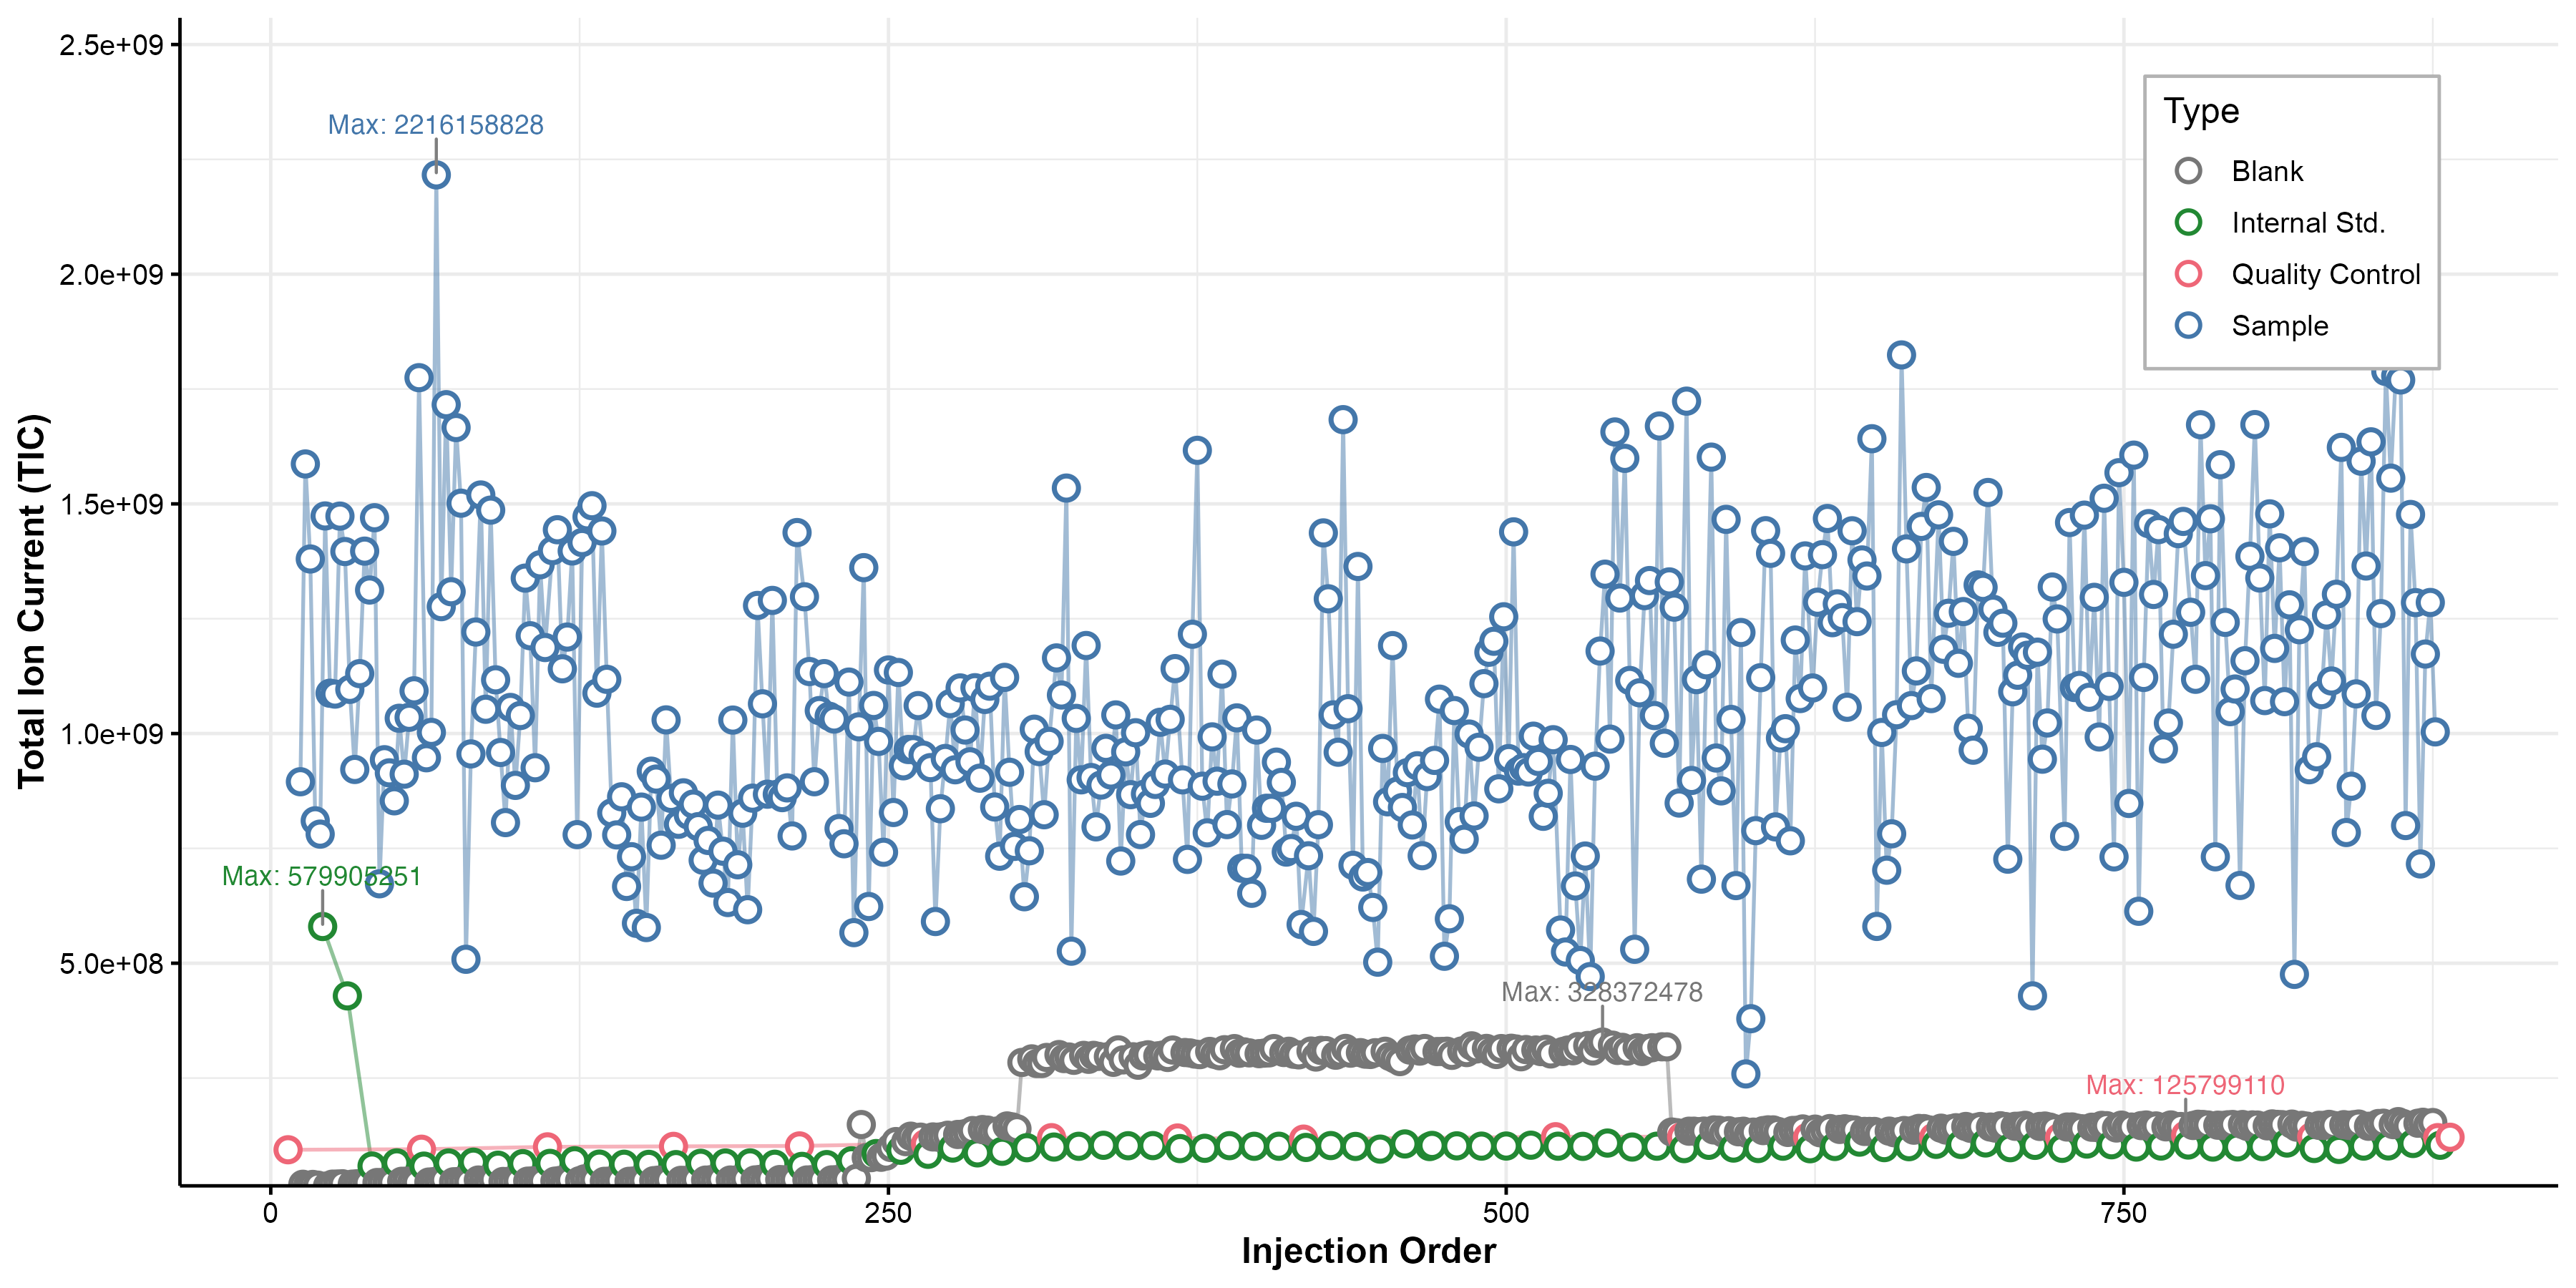
\includegraphics[width=\linewidth]{fig/supp/SuppFig_1A_TIC_Control}
    \caption{Total ion current vs.\ injection order for Control samples.}
    \label{fig:S1A}
  \end{subfigure}

  \vspace{1em}

  % ---------- panel B: Low-Input TIC ----------
  \begin{subfigure}[t]{\textwidth}
    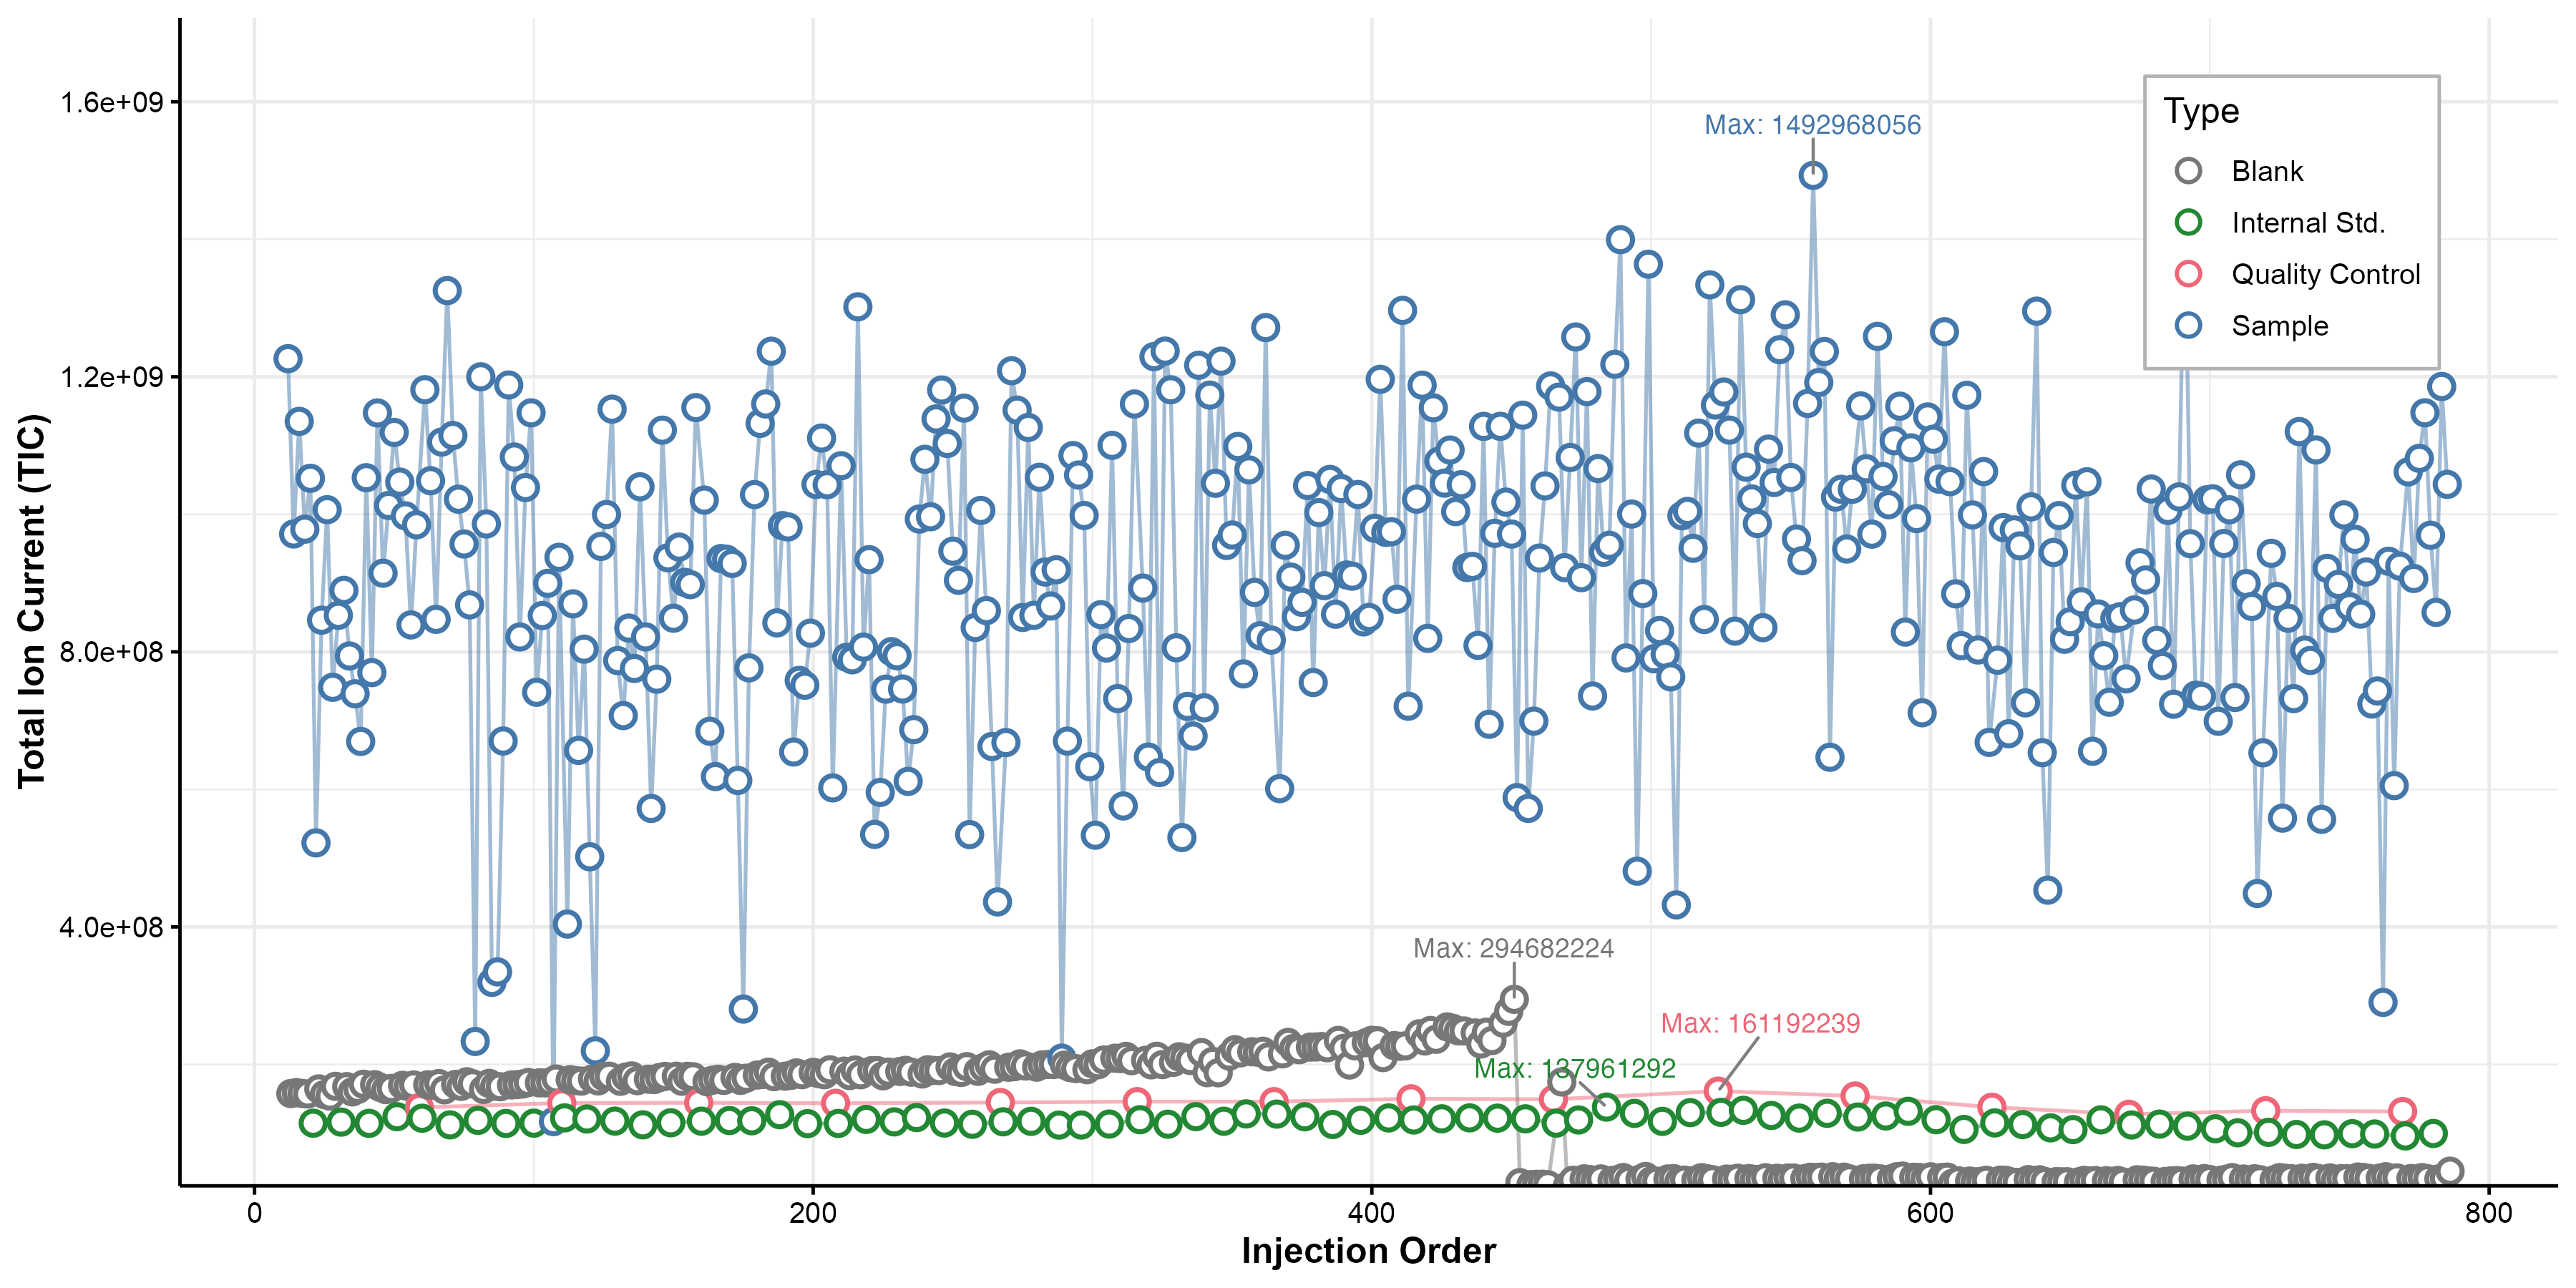
\includegraphics[width=\linewidth]{fig/supp/SuppFig_1B_TIC_LowInput.png}
    \caption{Total ion current vs.\ injection order for Low-Input samples.}
    \label{fig:S1B}
  \end{subfigure}

  \caption{TIC traces for all injections.  (A) Control, (B) Low-Input.}
  \label{fig:S1}
\end{figure}



%========================================================
%  Supplementary Figure S2 - SERFF RSD & PCA results
%========================================================
\begin{figure}[htp]
  \centering

  % ---------- row 1 ----------
  \begin{subfigure}[t]{0.48\textwidth}
    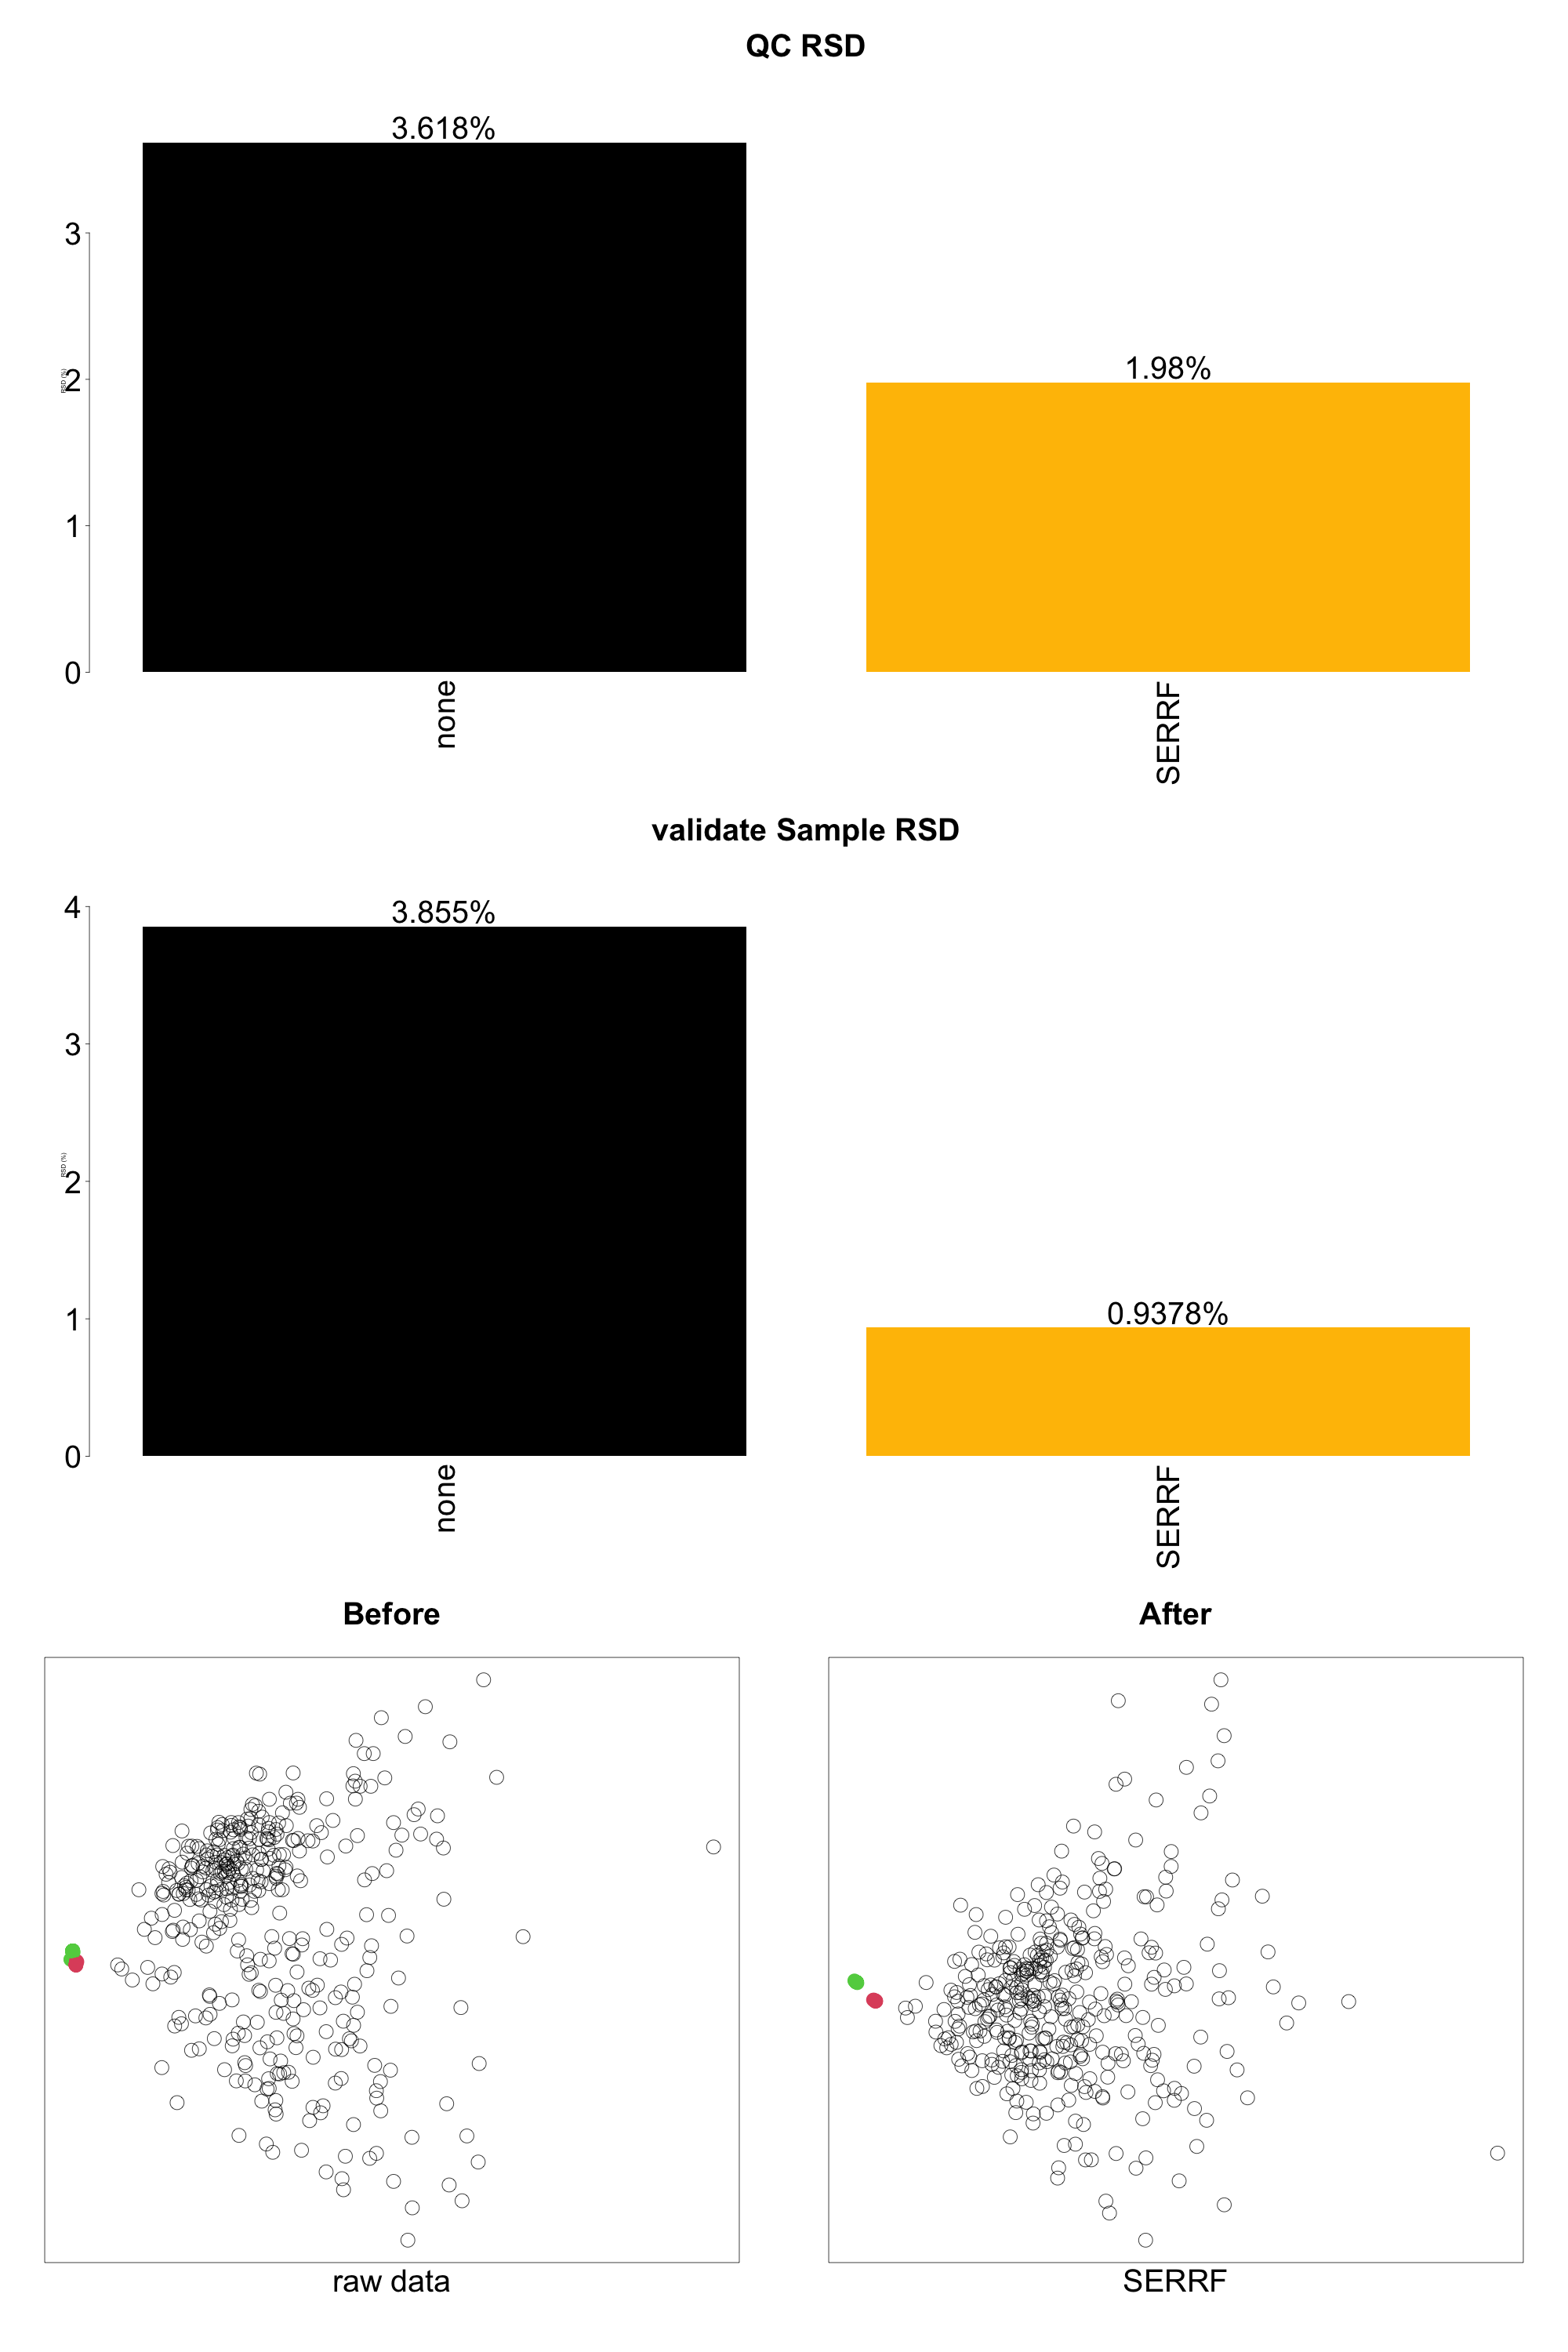
\includegraphics[width=\linewidth]{fig/supp/SuppFig_2A_RSD_PCA_Control.png}
    \caption{Control.}
    \label{fig:S2A}
  \end{subfigure}\hfill
  \begin{subfigure}[t]{0.48\textwidth}
    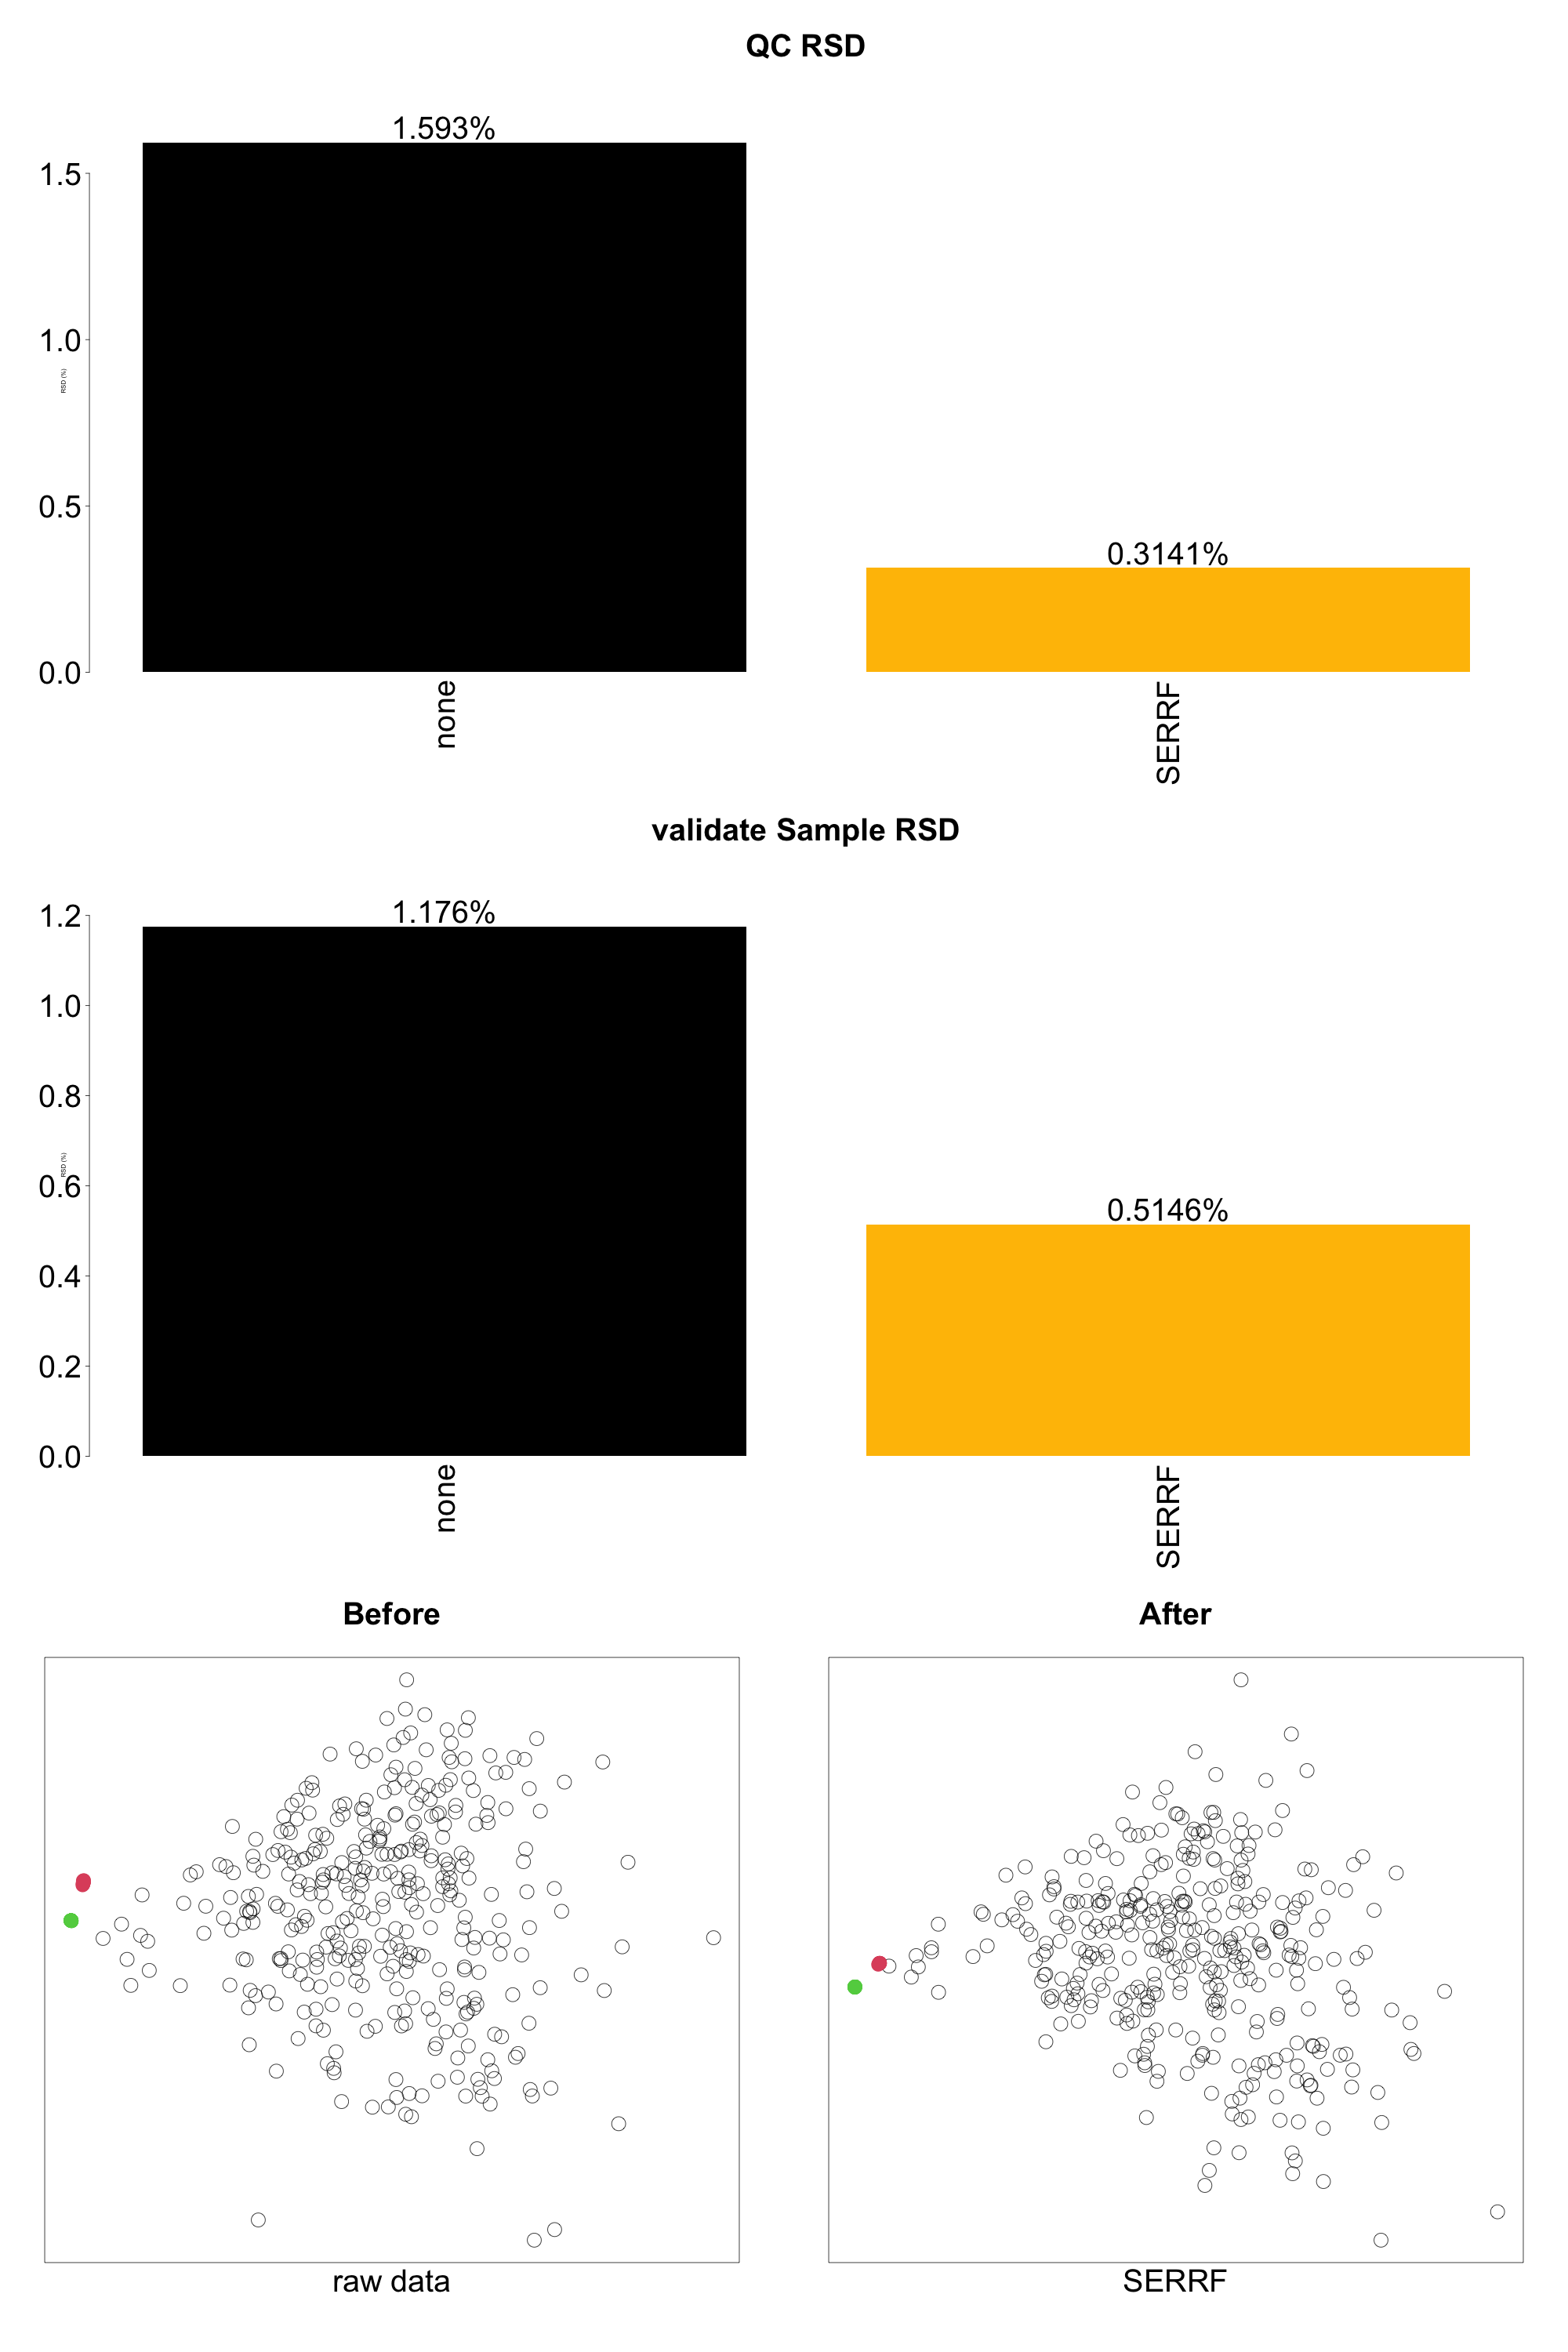
\includegraphics[width=\linewidth]{fig/supp/SuppFig_2B_RSD_PCA_Lowinput.png}
    \caption{Low‐Input.}
    \label{fig:S2B}
  \end{subfigure}

  \caption{
    SERRF-normalized quality metrics across injections.  
    (\textbf{A}) Control samples: per‐feature RSD distributions (boxplot) and PCA of QC vs.\ samples.  
    (\textbf{B}) Low‐Input samples: same metrics after SERRF correction.  
    Both panels demonstrate tight RSDs (most features<15 %) and clear separation of QC from biological samples in PC1/PC2.
  }
  \label{fig:S2}
\end{figure}







%========================================================
%  Supplementary Figure S3 - Lipid species/class count   (panels A, B, C, and D)
%========================================================
\begin{figure}[htp]
  \centering

  % ---------- row 1 ----------
  \begin{subfigure}[t]{0.48\textwidth}
    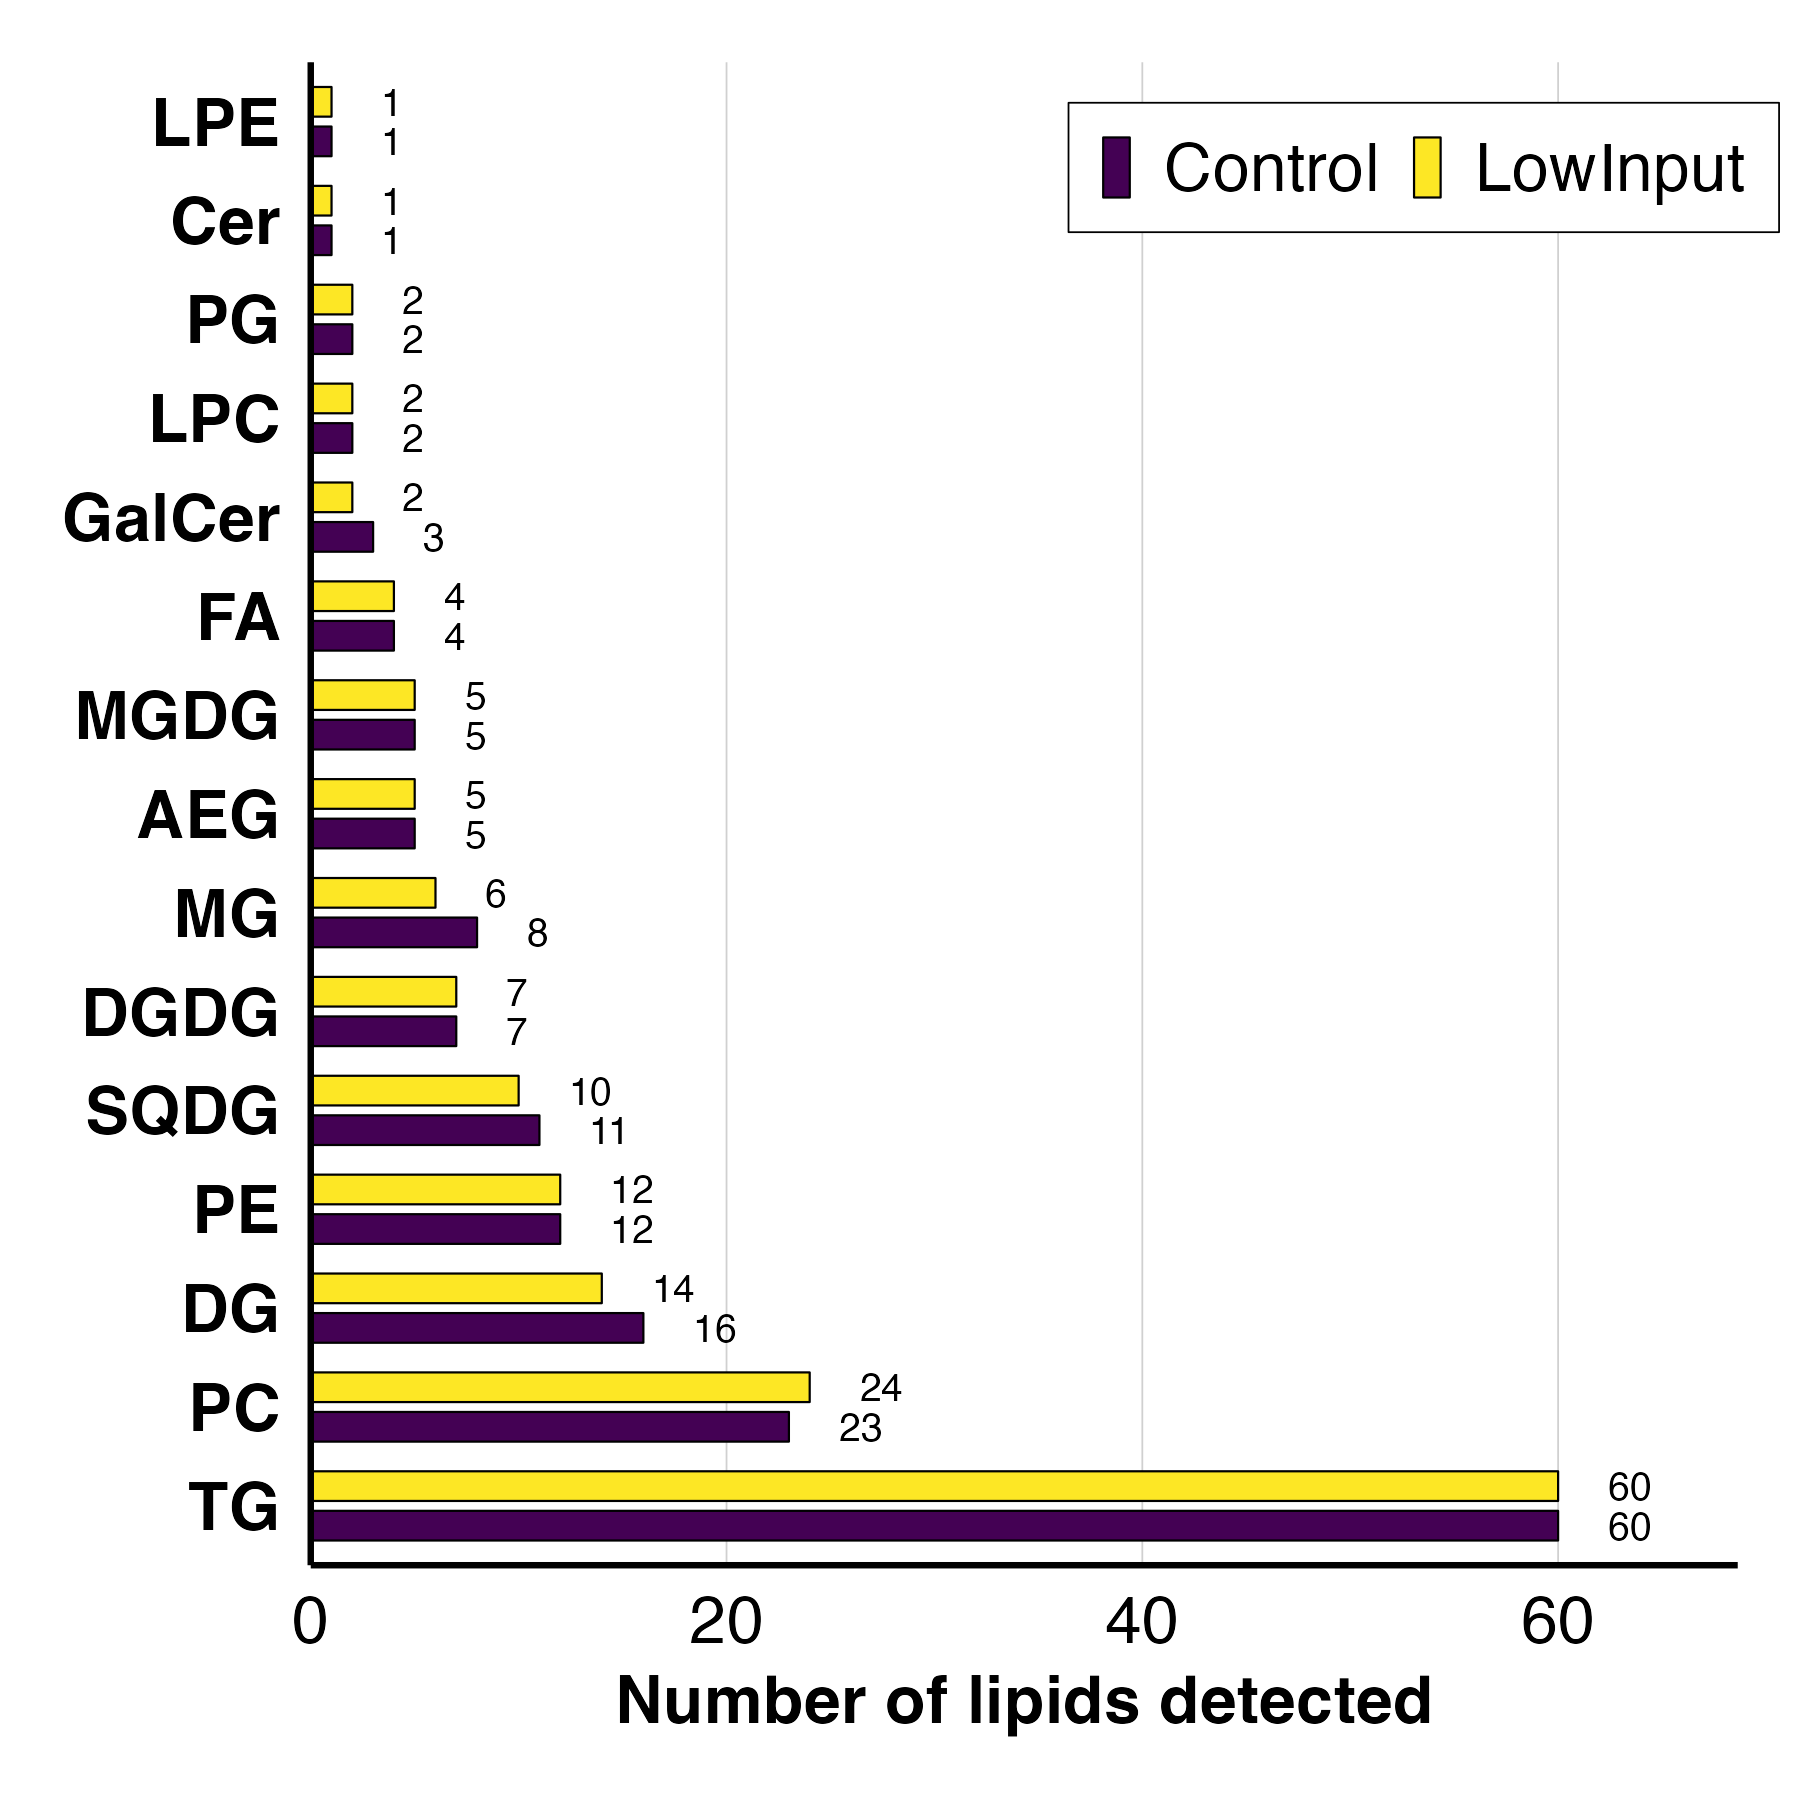
\includegraphics[width=\linewidth]{fig/supp/SuppFig_3A_Lipid_Counts.png}
    \caption{Number of lipid \textit{species}.}
    \label{fig:S3A}
  \end{subfigure}\hfill
  \begin{subfigure}[t]{0.48\textwidth}
    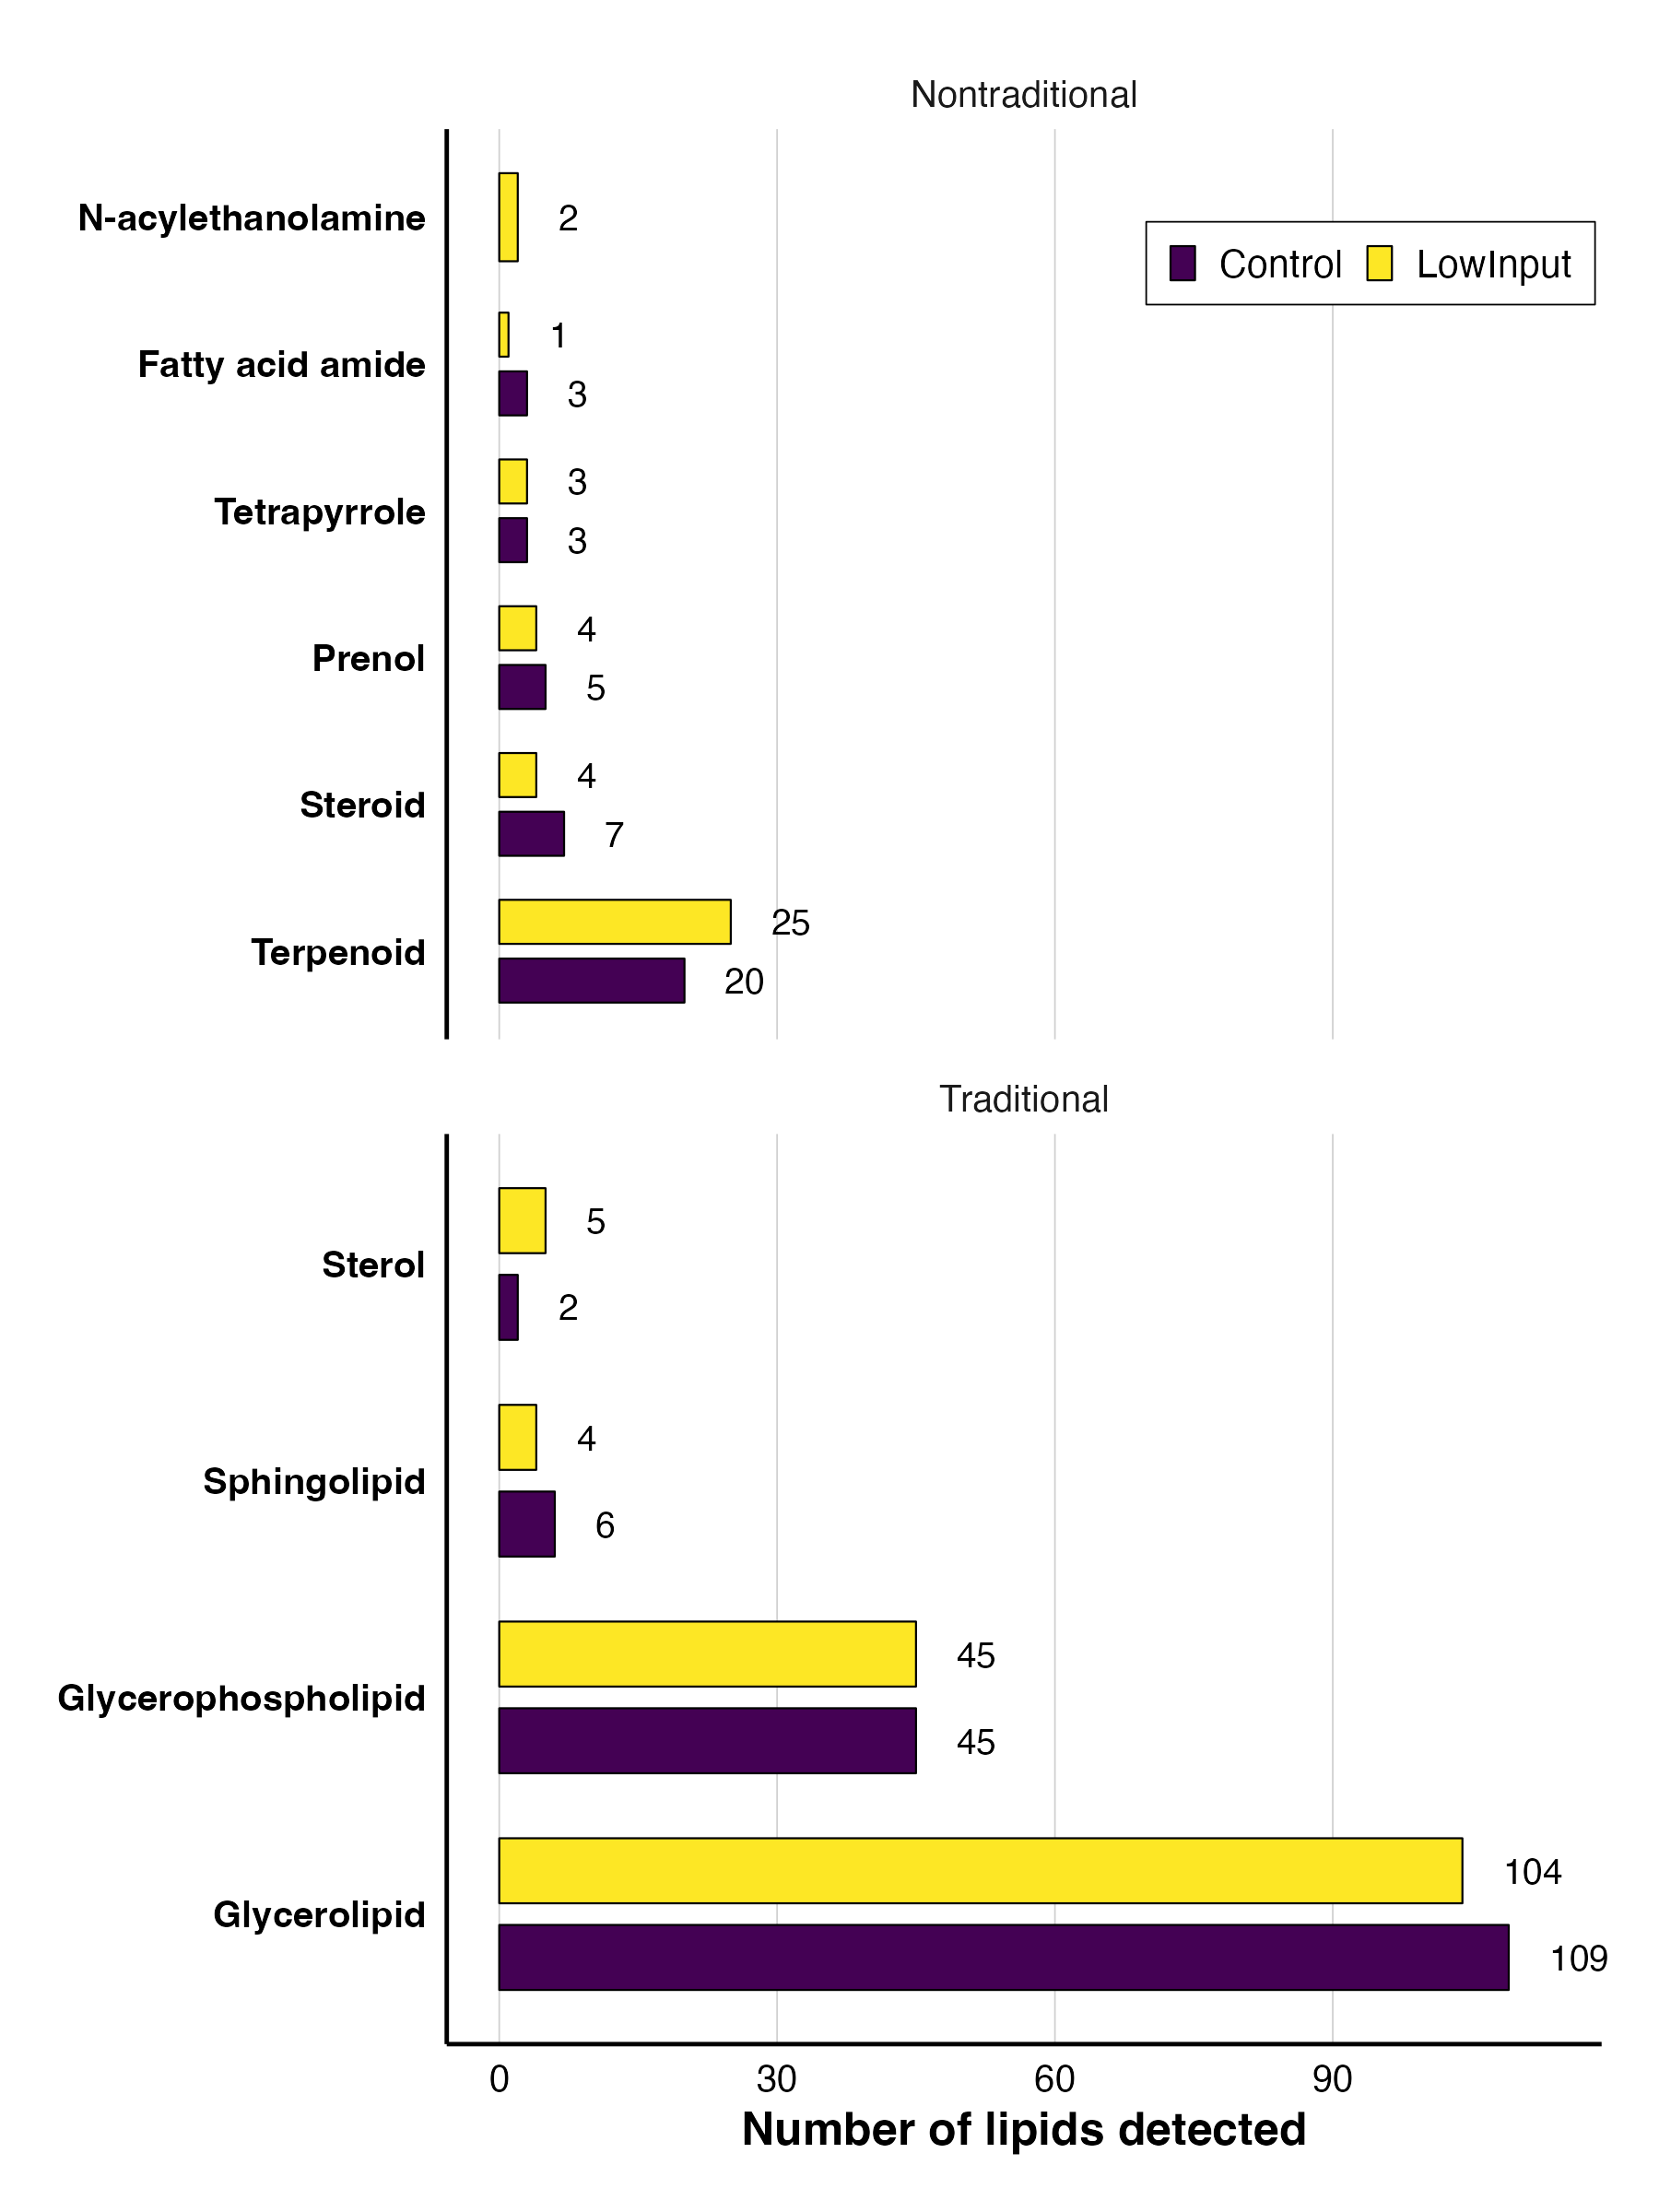
\includegraphics[width=\linewidth]{fig/supp/SuppFig_3B_trad_nontrad_counts.png}
    \caption{Number of lipid \textit{classes}.}
    \label{fig:S3B}
  \end{subfigure}

  \vspace{1em}

  % ---------- row 2 ----------
  \begin{subfigure}[t]{0.48\textwidth}
    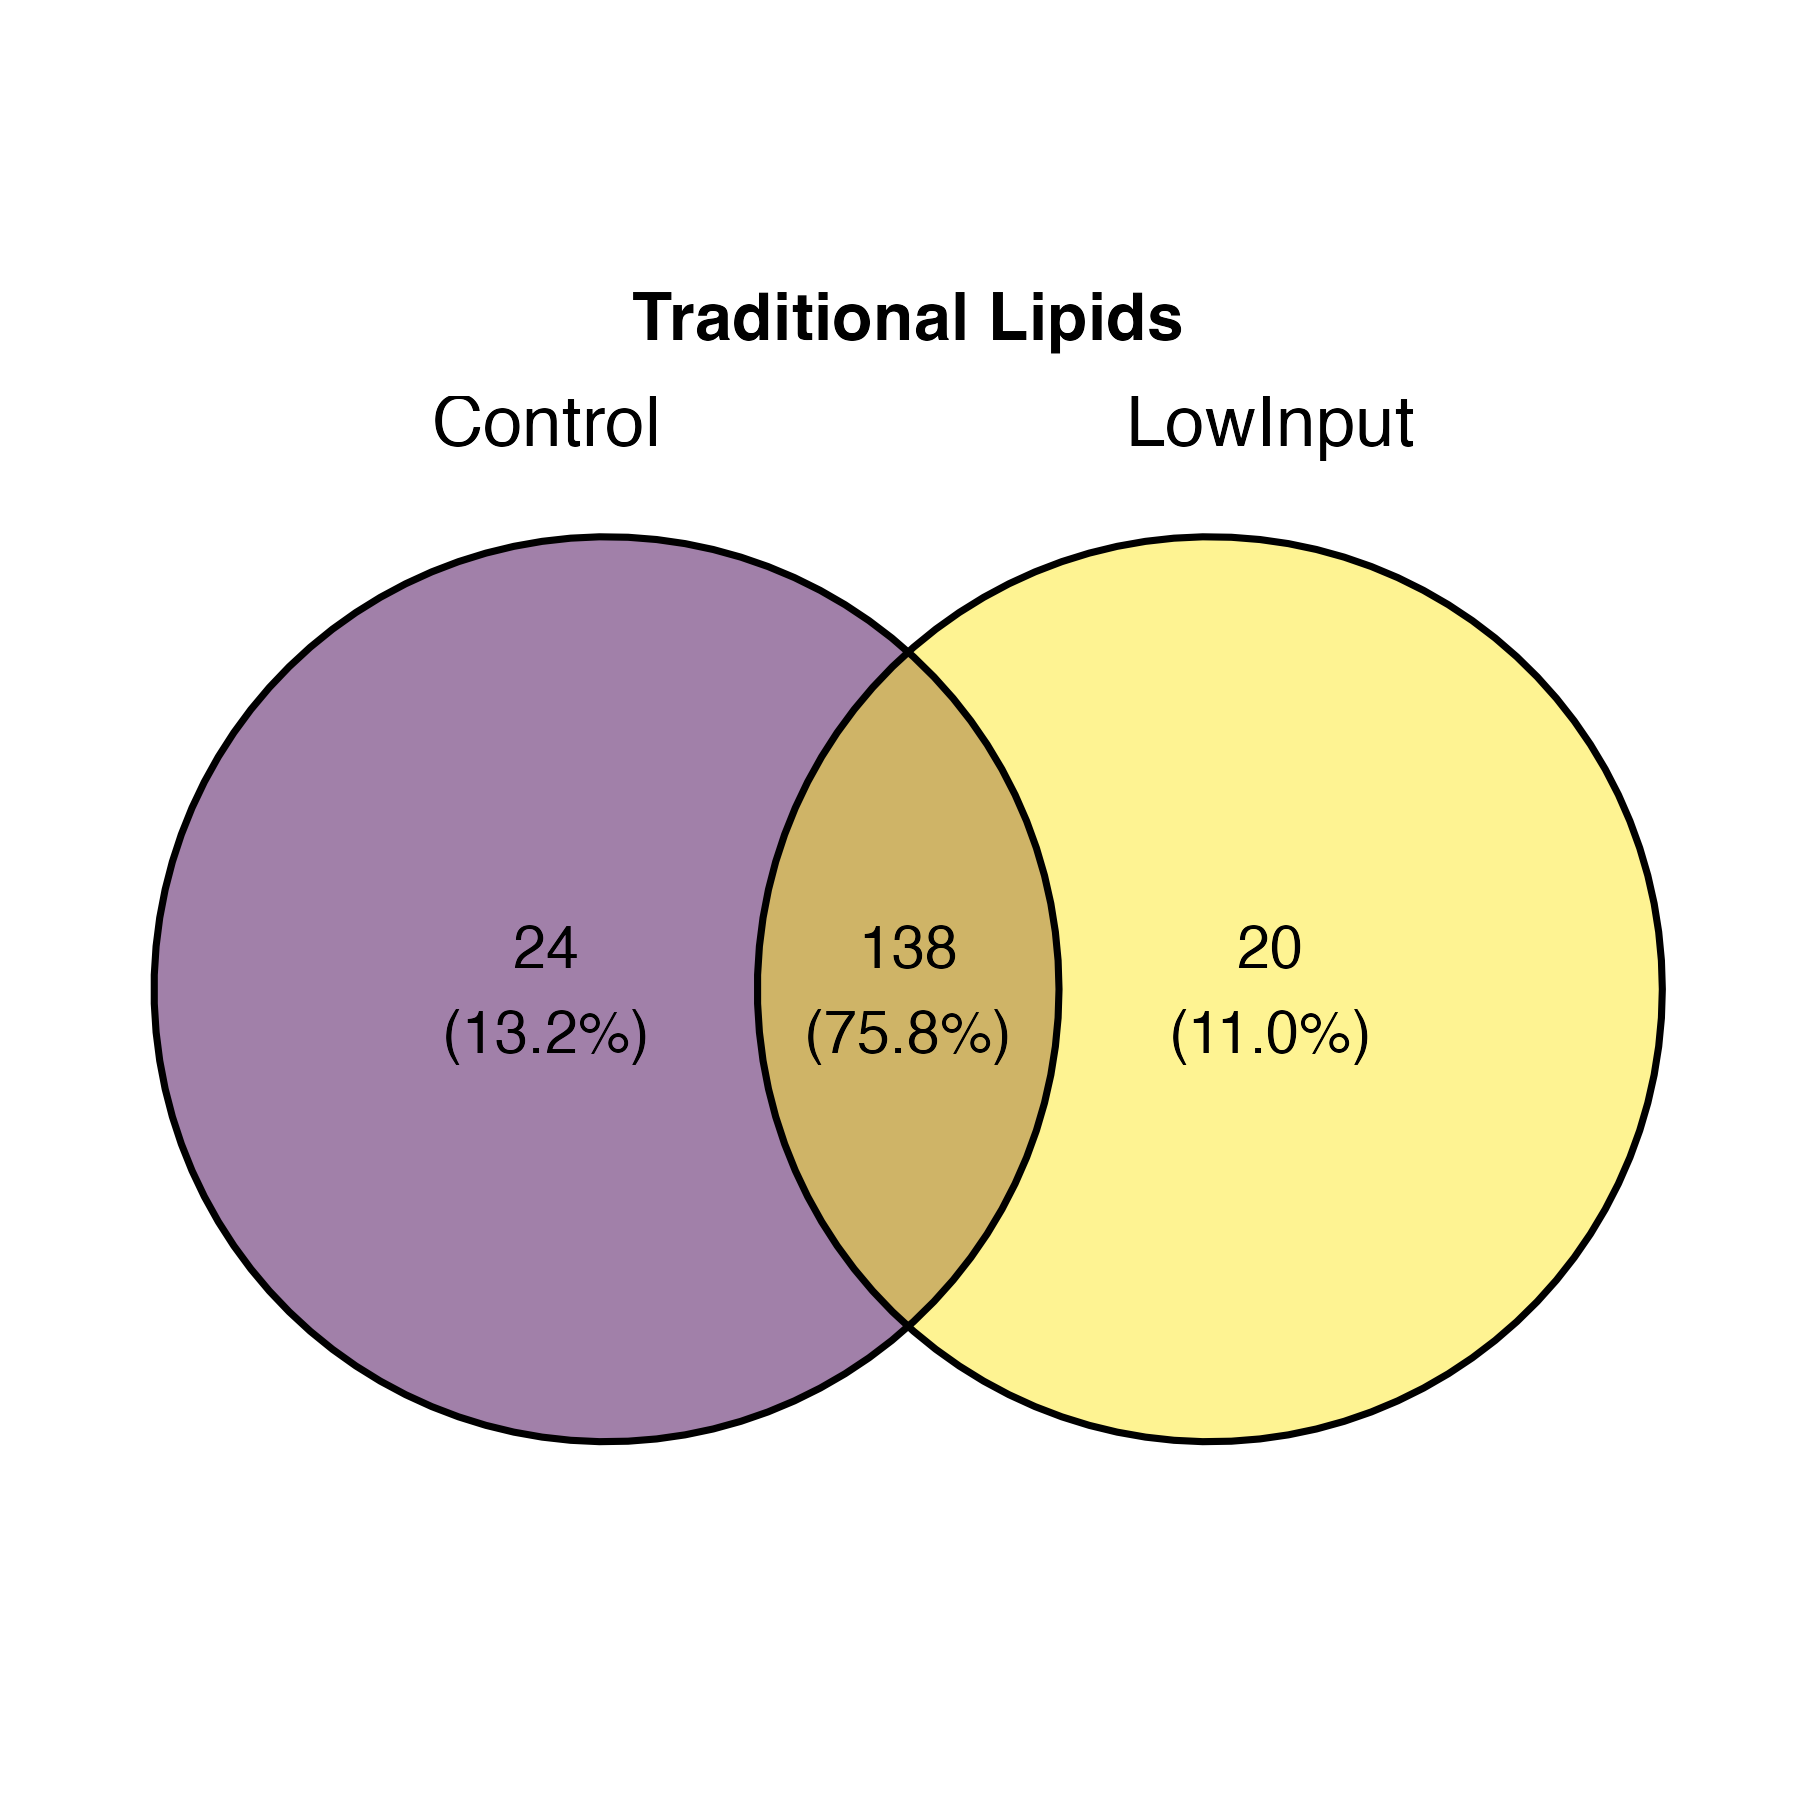
\includegraphics[width=\linewidth]{fig/supp/SuppFig_3C_Lipid_Overlap_Venn_traditional.png}
    \caption{Shared and unique traditional lipid species.}
    \label{fig:S3C}
  \end{subfigure}\hfill
  \begin{subfigure}[t]{0.48\textwidth}
    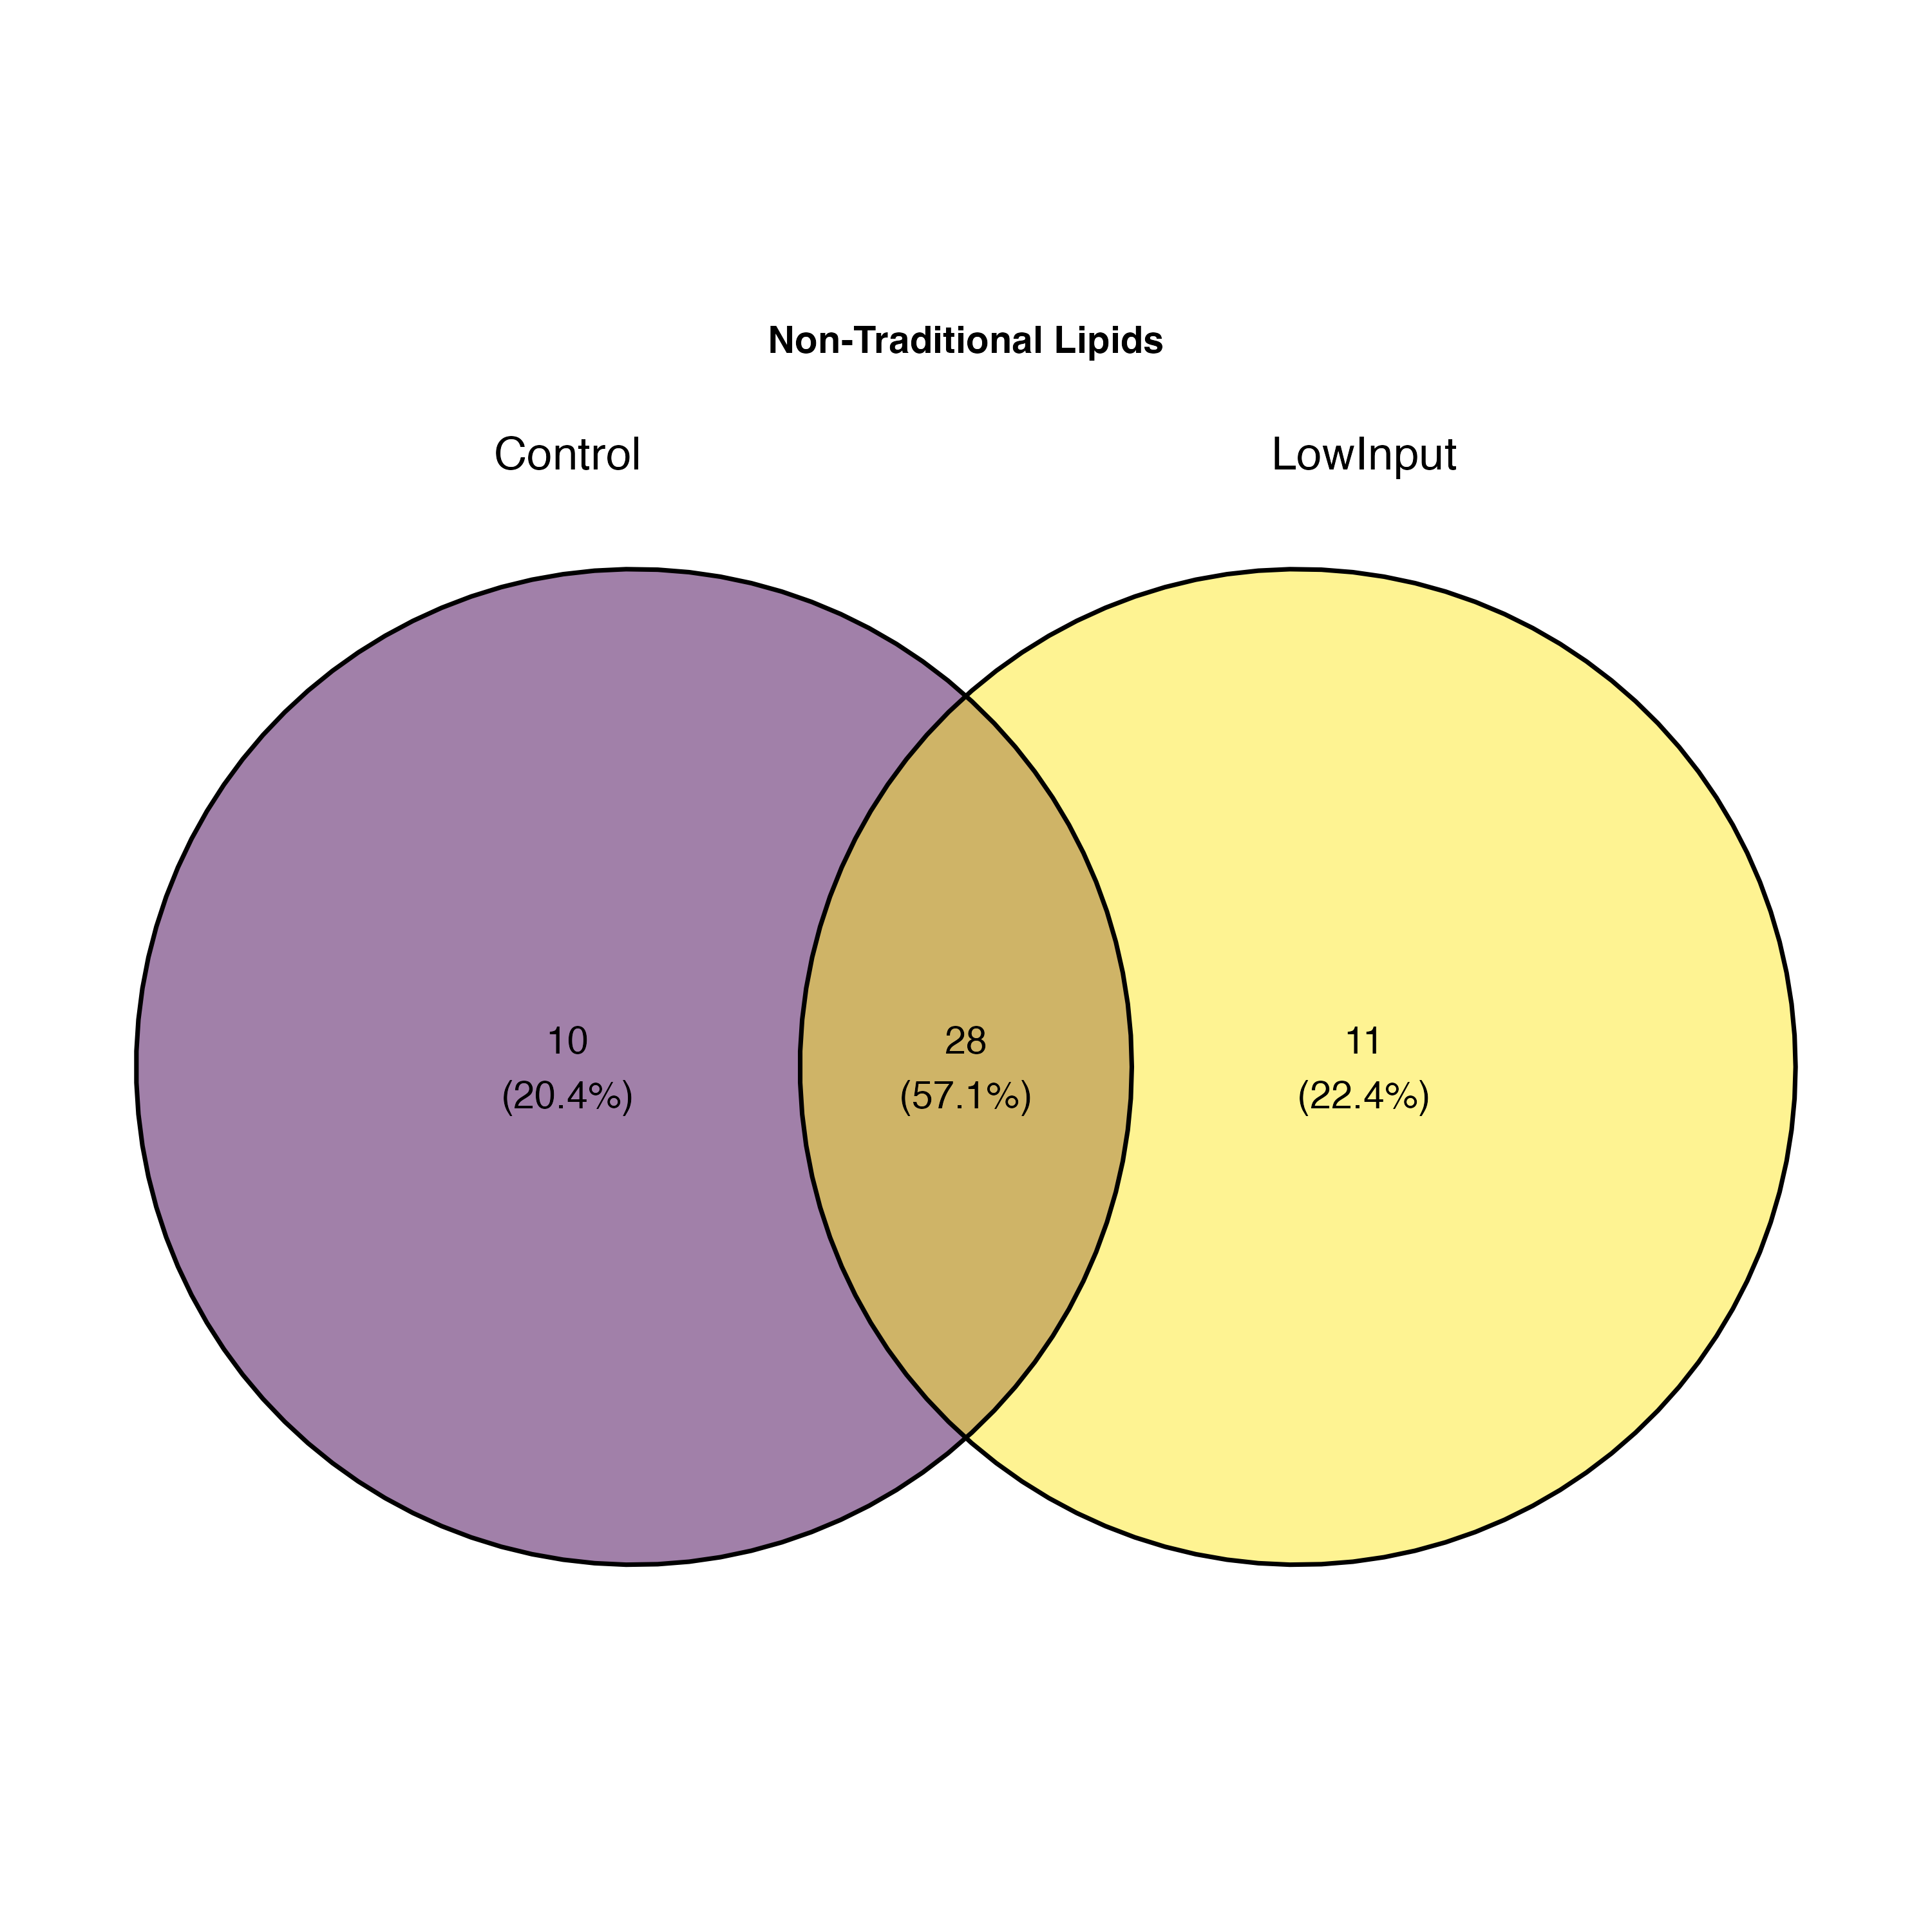
\includegraphics[width=\linewidth]{fig/supp/SuppFig_3D_Lipid_Overlap_Venn_nontraditional.png}
    \caption{Shared and unique non-traditional lipid species.}
    \label{fig:S3D}
  \end{subfigure}

  \caption{Overview of lipid coverage in C and LI samples.}
  \label{fig:S3}
\end{figure}



%\begin{figure}[htp]
%  \centering

  % ---------- row 1 ----------
  %\begin{subfigure}[t]{0.48\textwidth}
  %  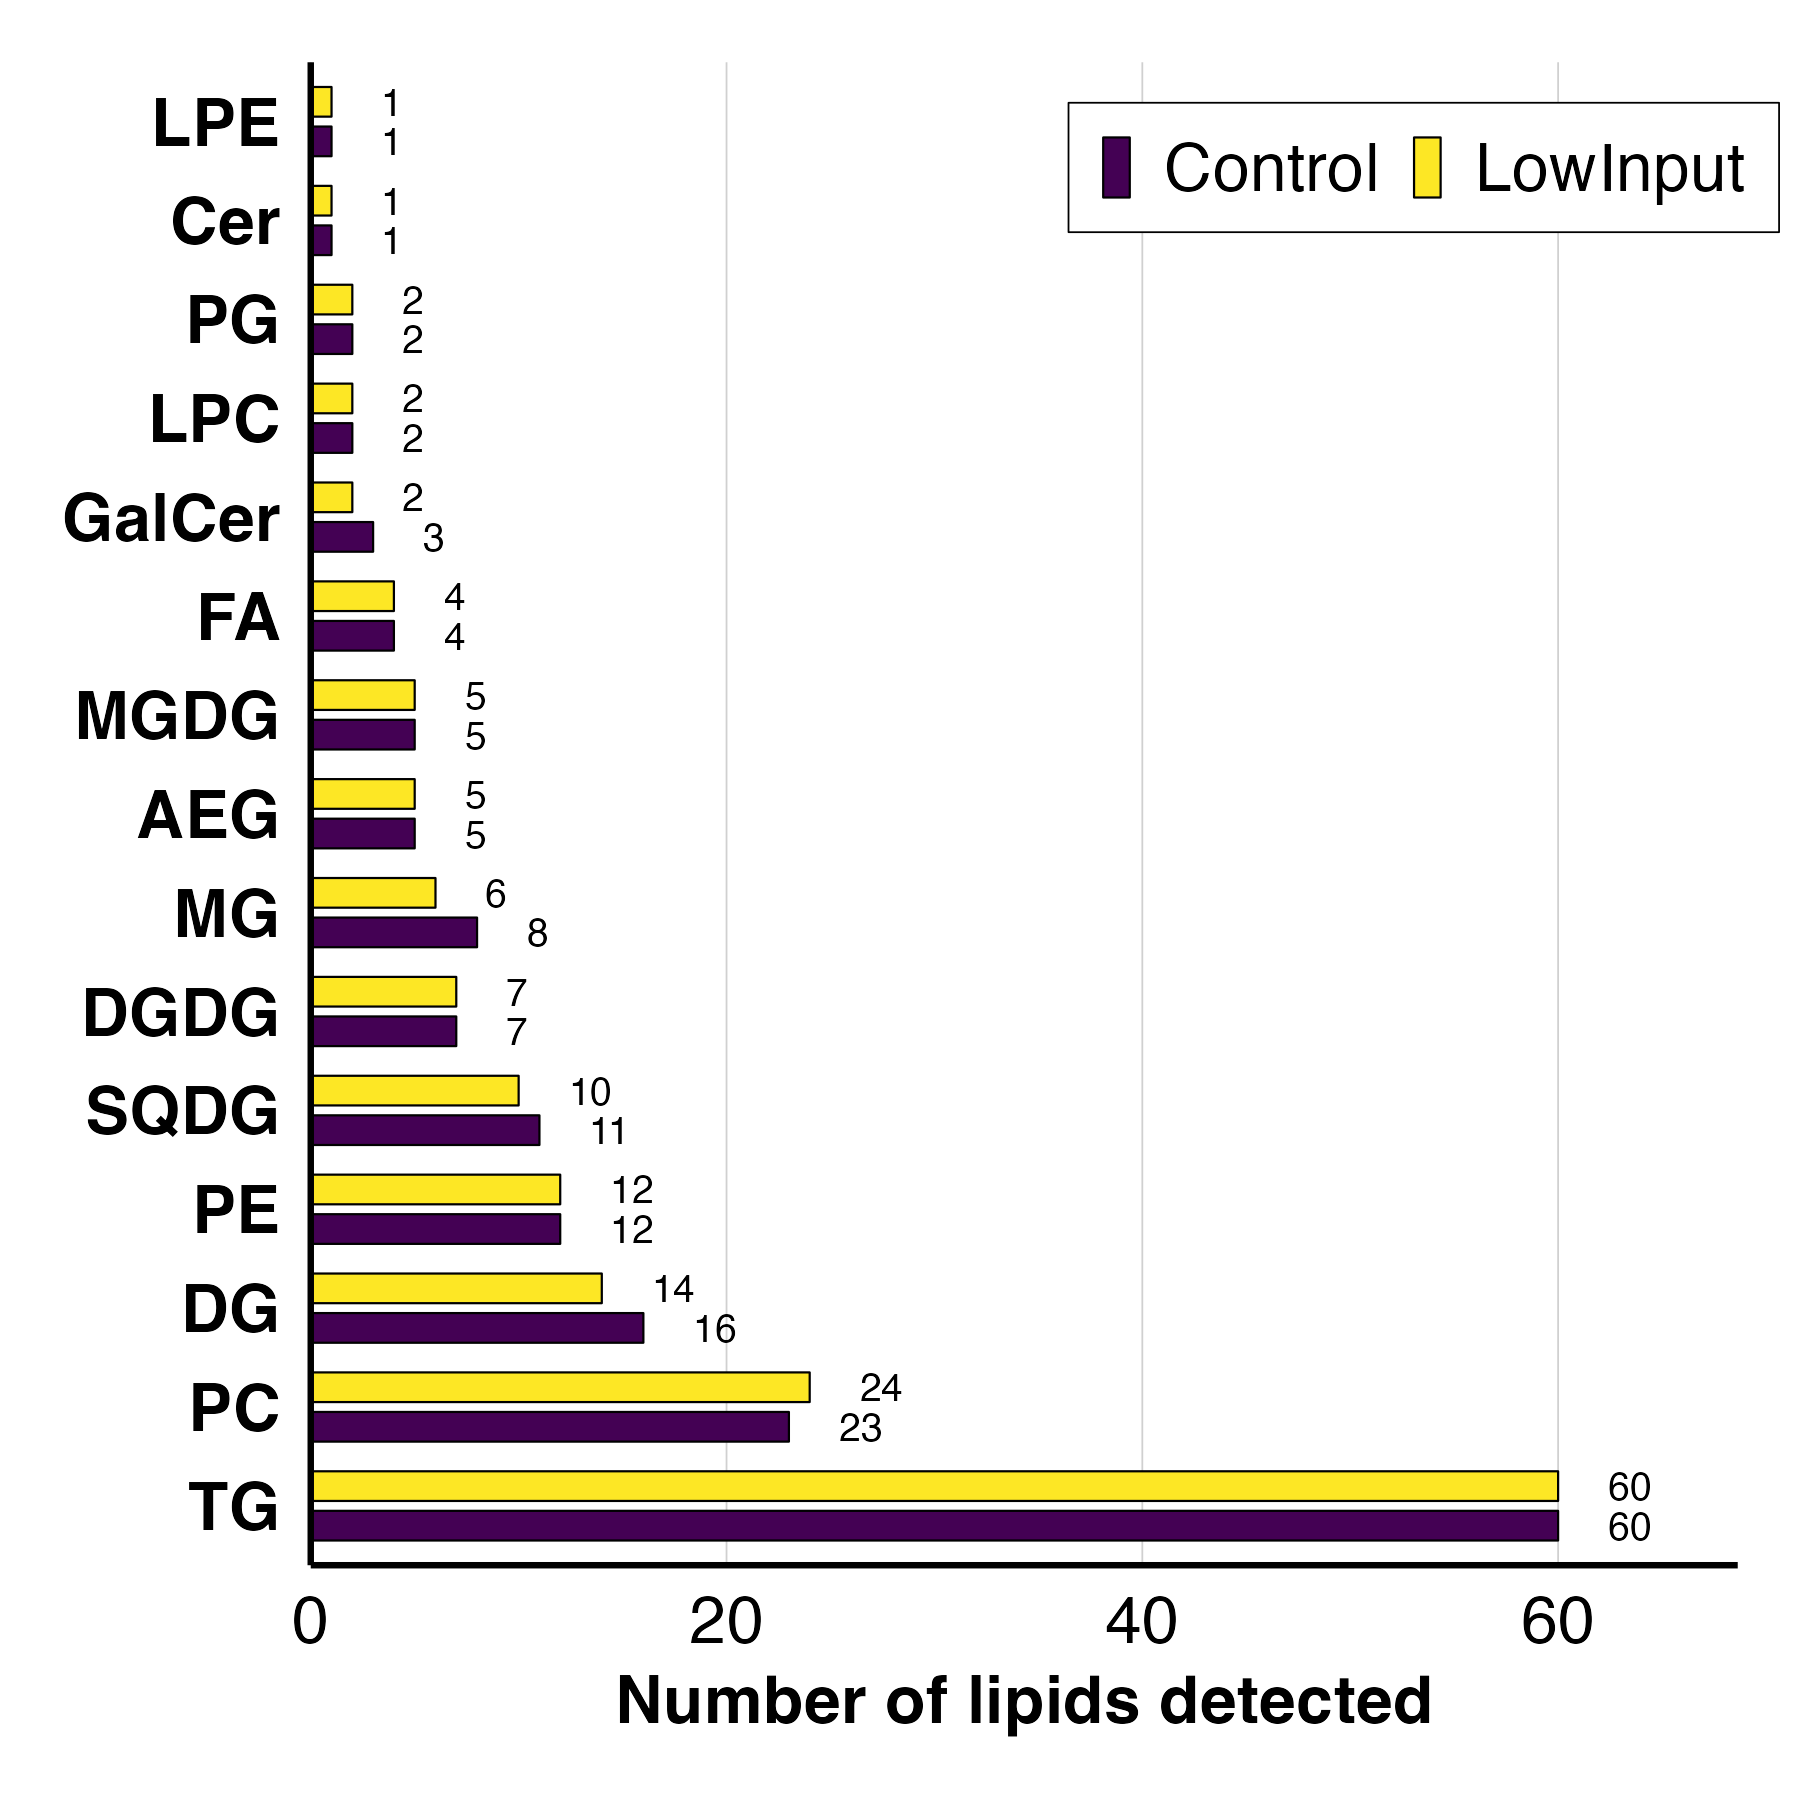
\includegraphics[width=\linewidth]{fig/supp/SuppFig_3A_Lipid_Counts.png}
  %  \caption{Number of lipid \textit{species}.}
  %  \label{fig:S3A}
  %\end{subfigure}\hfill
  %\begin{subfigure}[t]{0.48\textwidth}
  %  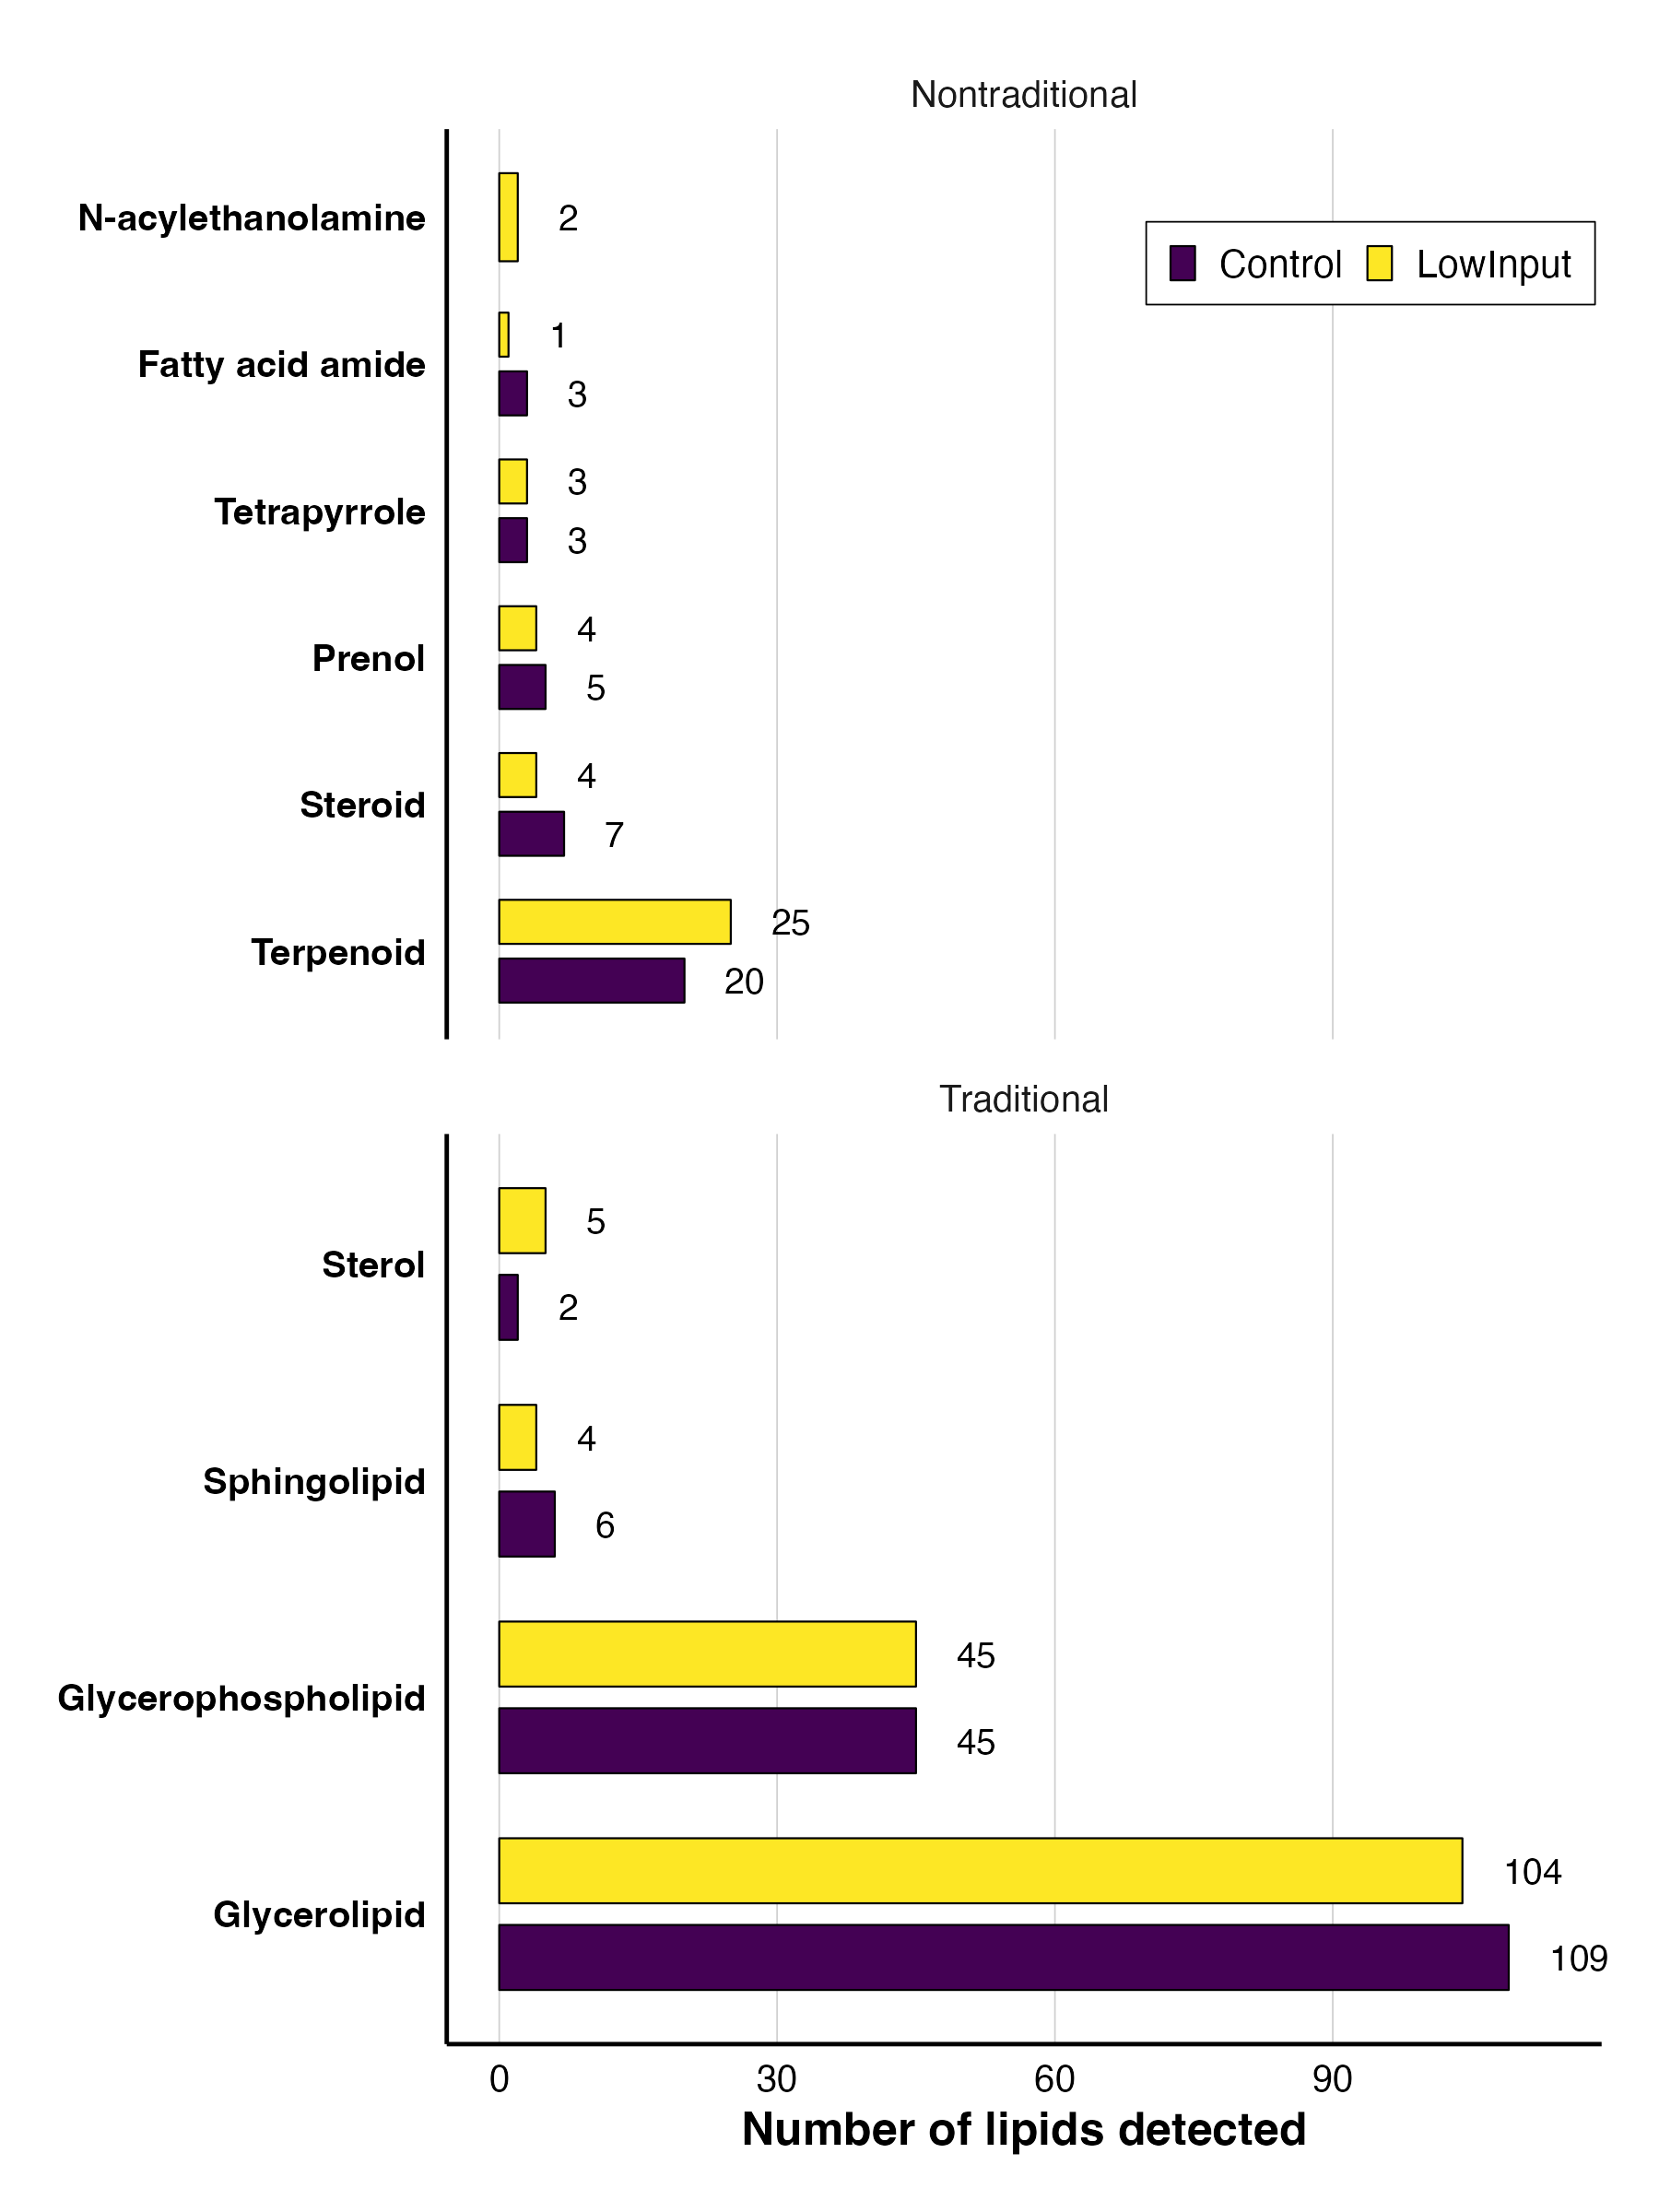
\includegraphics[width=\linewidth]{fig/supp/SuppFig_3B_trad_nontrad_counts.png}
  %  \caption{Number of lipid \textit{classes}.}
  %  \label{fig:S3B}
  %\end{subfigure}

  %\vspace{1em}

  % ---------- row 2 (centred) ----------
  %\begin{subfigure}[t]{0.55\textwidth}
  %  \centering
  %  \includegraphics[width=\linewidth]%{fig/supp/SuppFig_3C_Lipid_Overlap_Venn_traditional.png}
    %\caption{Shared and unique lipid species.}
    %\label{fig:S3C}
  %\end{subfigure}

  %\caption{Overview of lipid coverage in Control and Low-Input samples.}
  %\label{fig:S3}
%\end{figure}



%========================================================
%  Supplementary Figure S4 - Lipid ratio contrasts under low-P
%========================================================
\begin{figure}[htp]
  \centering
  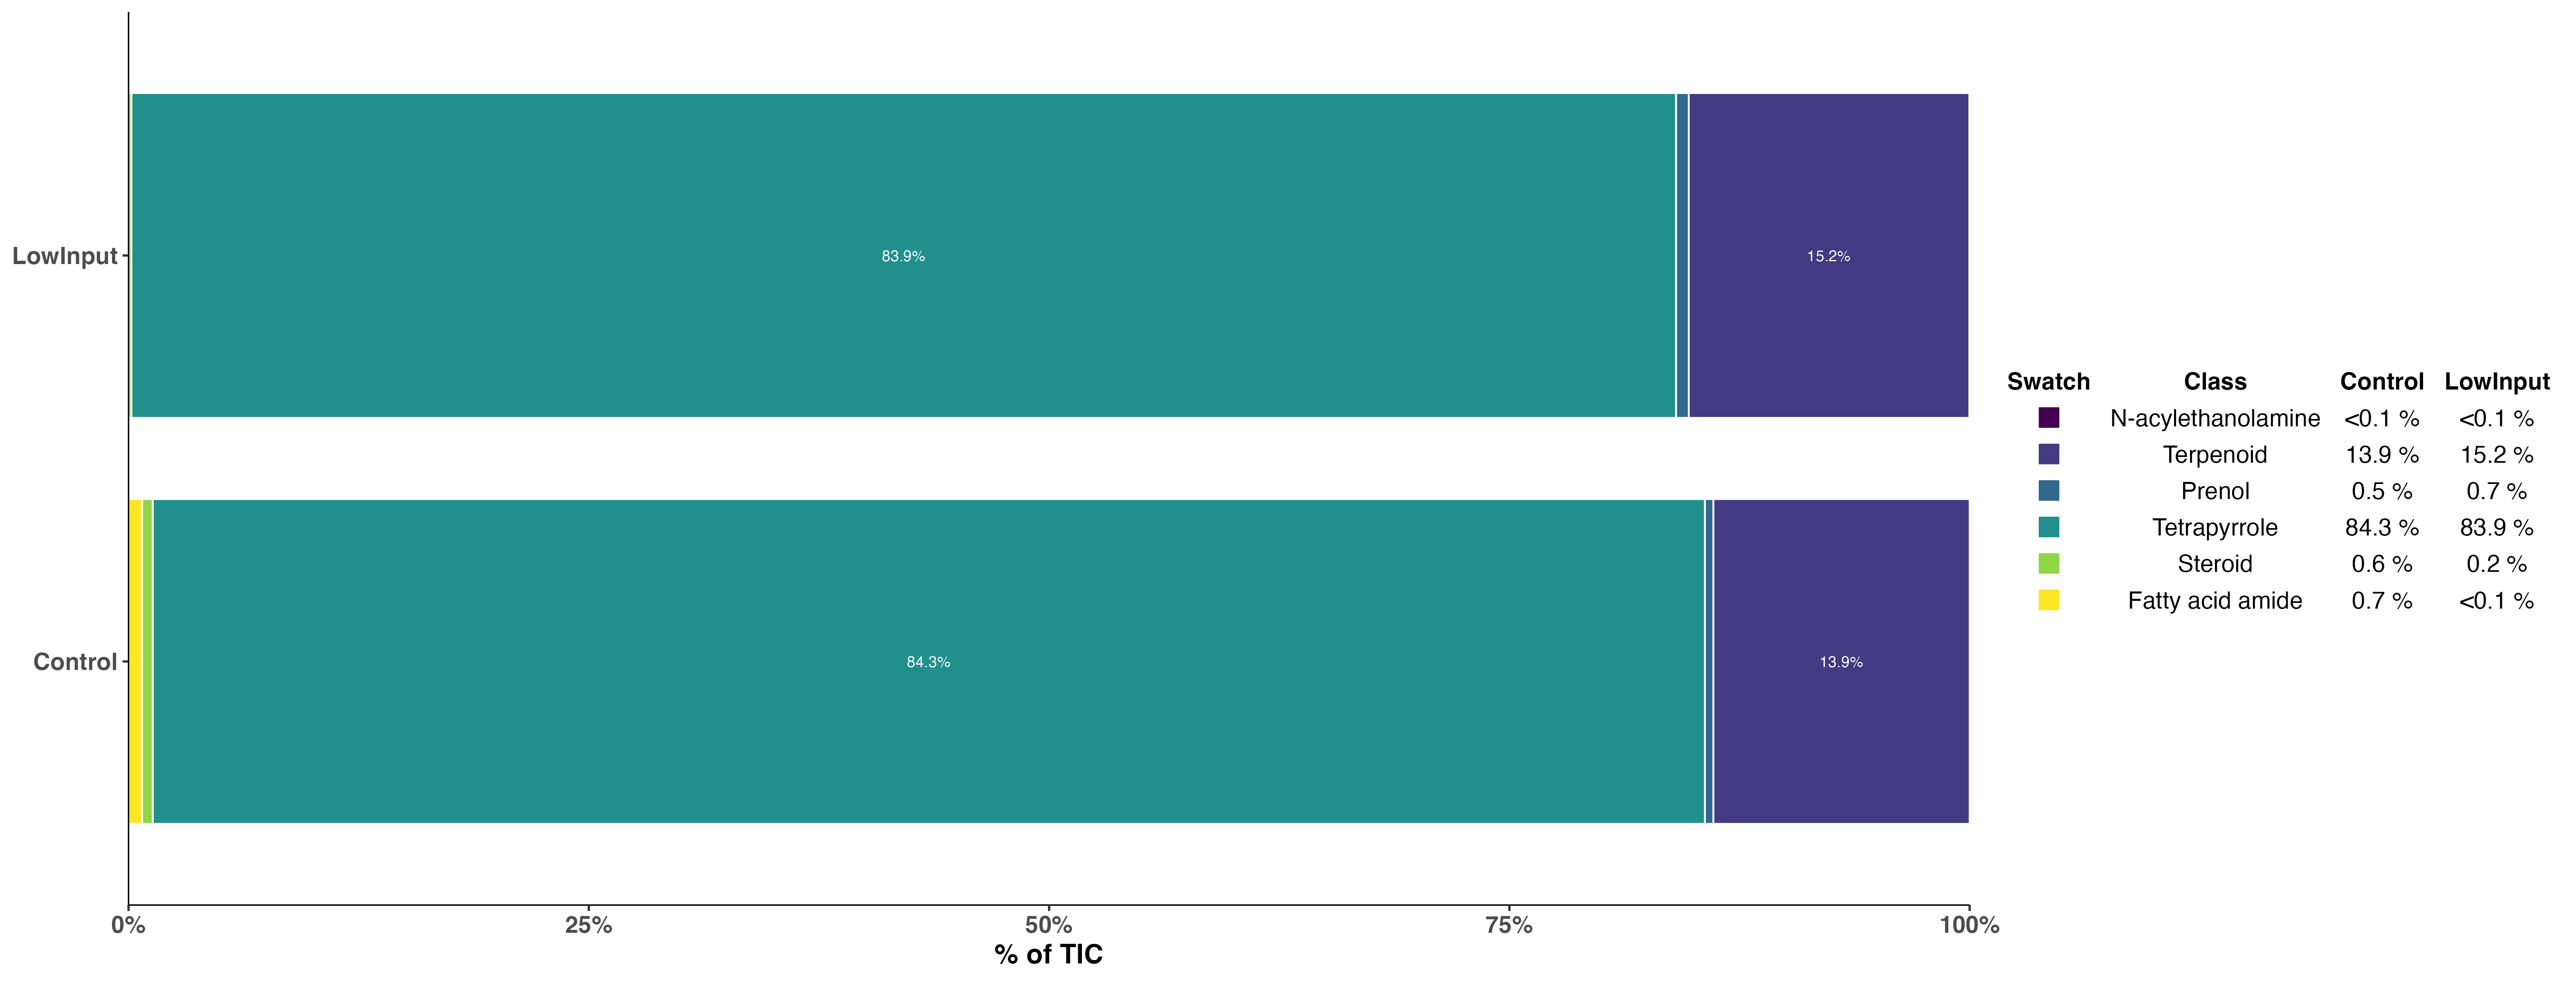
\includegraphics[width=0.65\textwidth]{fig/supp/SuppFig_4_TIC_nontraditional_lipid_class.png}
  \caption{Relative contribution of non-traditional lipid classes to total ion current (TIC) under Control and Low-Input conditions. Classes contributing less than 3\% in both conditions were omitted for clarity.}
  \label{fig:S4_TIC_nontraditional}
\end{figure}



%========================================================
%  Supplementary Figure S4 - Lipid ratio contrasts under low-P
%========================================================
\begin{figure}[htp]
  \centering
  % Adjust width fraction as needed (e.g., 0.8\textwidth or \textwidth)
  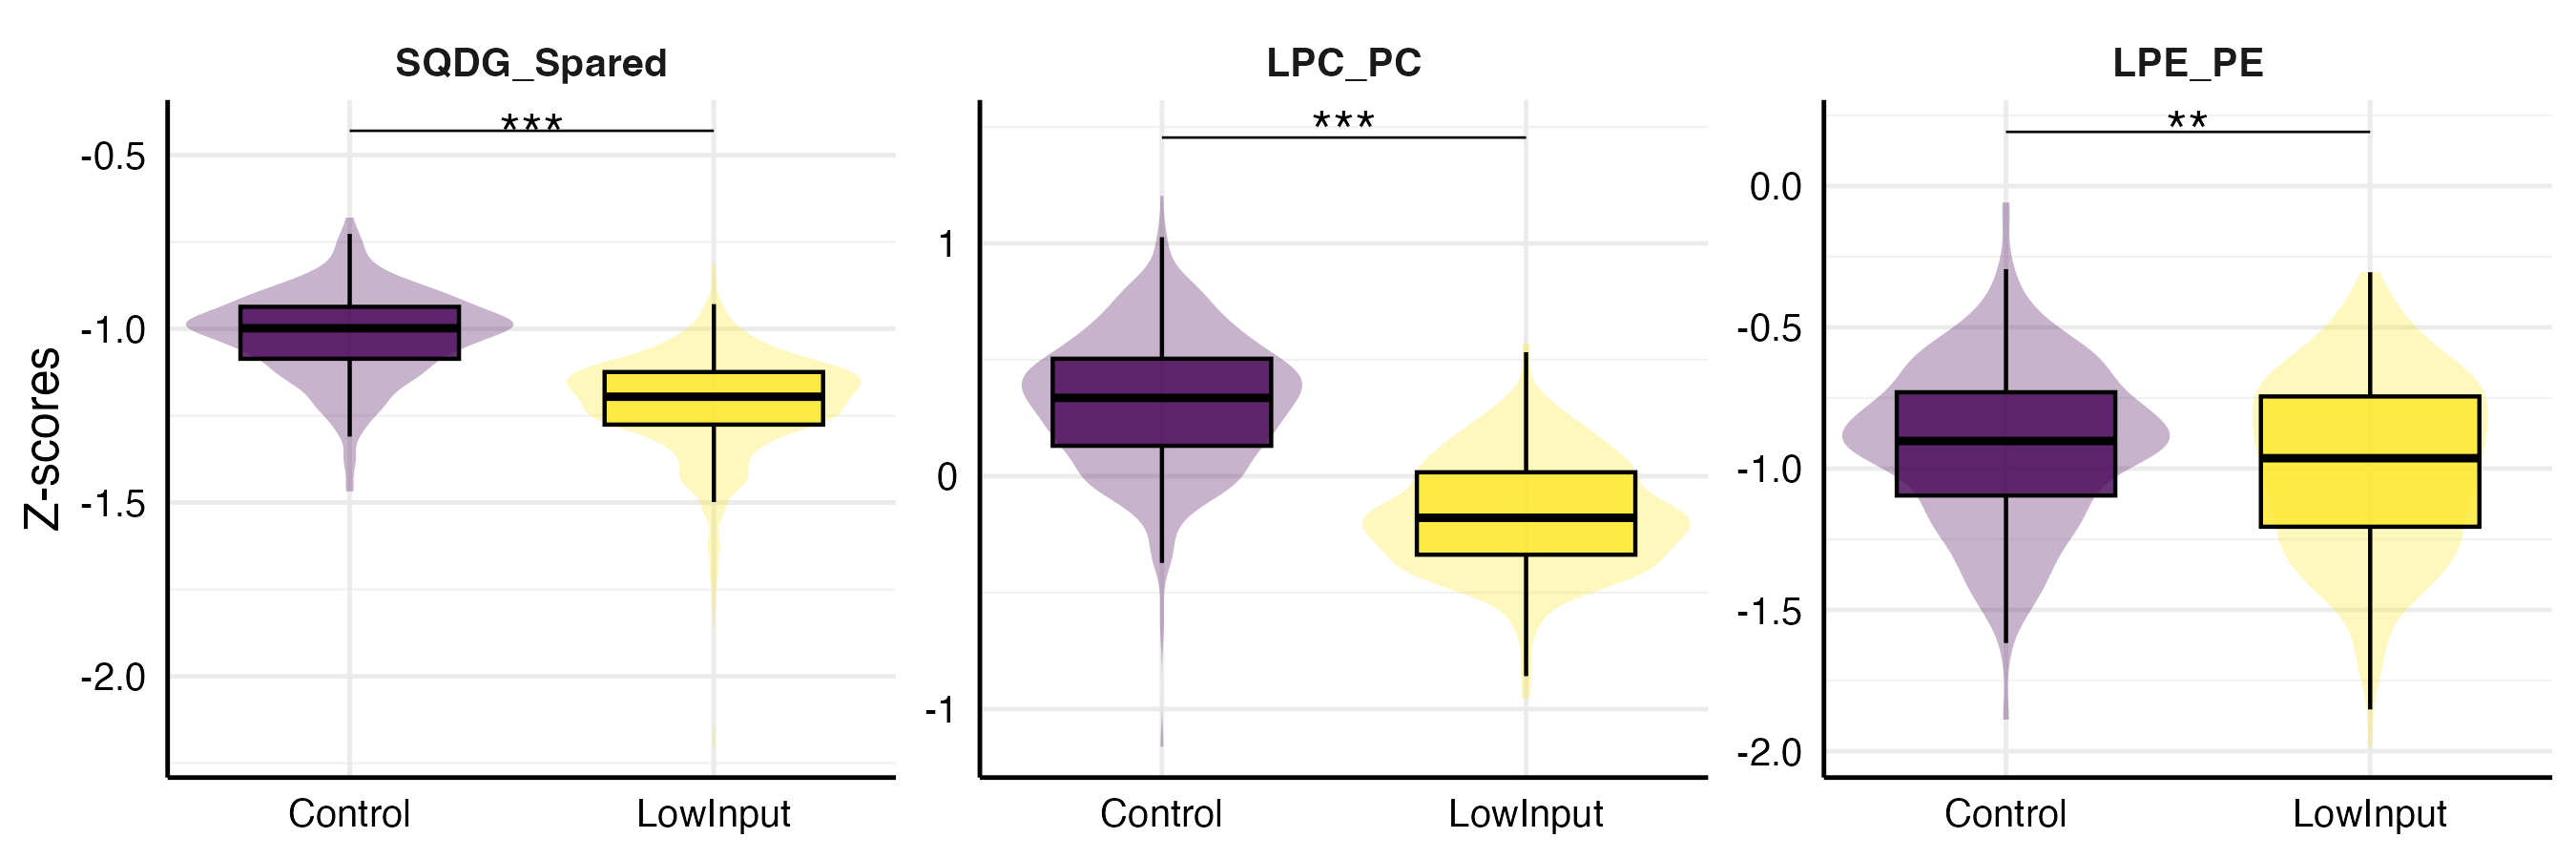
\includegraphics[width=0.8\textwidth]{fig/supp/SuppFig_4_lipid_ratio_linear_lowP.png}
  \caption{$\Delta$Z-score contrasts for lipids under LI. 
    The panel shows violin+boxplots for metrics such as \textitt{SQDG-Spared}, \textitt{LPC-PC}, and \textitt{LPE-PE} under Control versus LowInput conditions. 
    Stars denote significance levels (***: $p<0.001$, **: $p<0.01$, *: $p<0.05$) from appropriate statistical tests. 
    A negative $\Delta$Z in SQDG\_Spared indicates sulfolipid is not upregulated relative to galactolipids and PG; 
    \textitt{LPC-PC} is not significantly changed, whereas \textitt{LPE-PE} and composite Lyso\_activity shift toward values consistent with selective PE deacylation.}
  \label{fig:S4_lipid_ratio_lowP}
\end{figure}

%========================================================
%  Supplementary Figure S5 - TIC Proportions for LPC and LPE
%========================================================
\begin{figure}[htp]
  \centering
  % Adjust width fraction as appropriate, e.g., 0.6\textwidth or \textwidth
  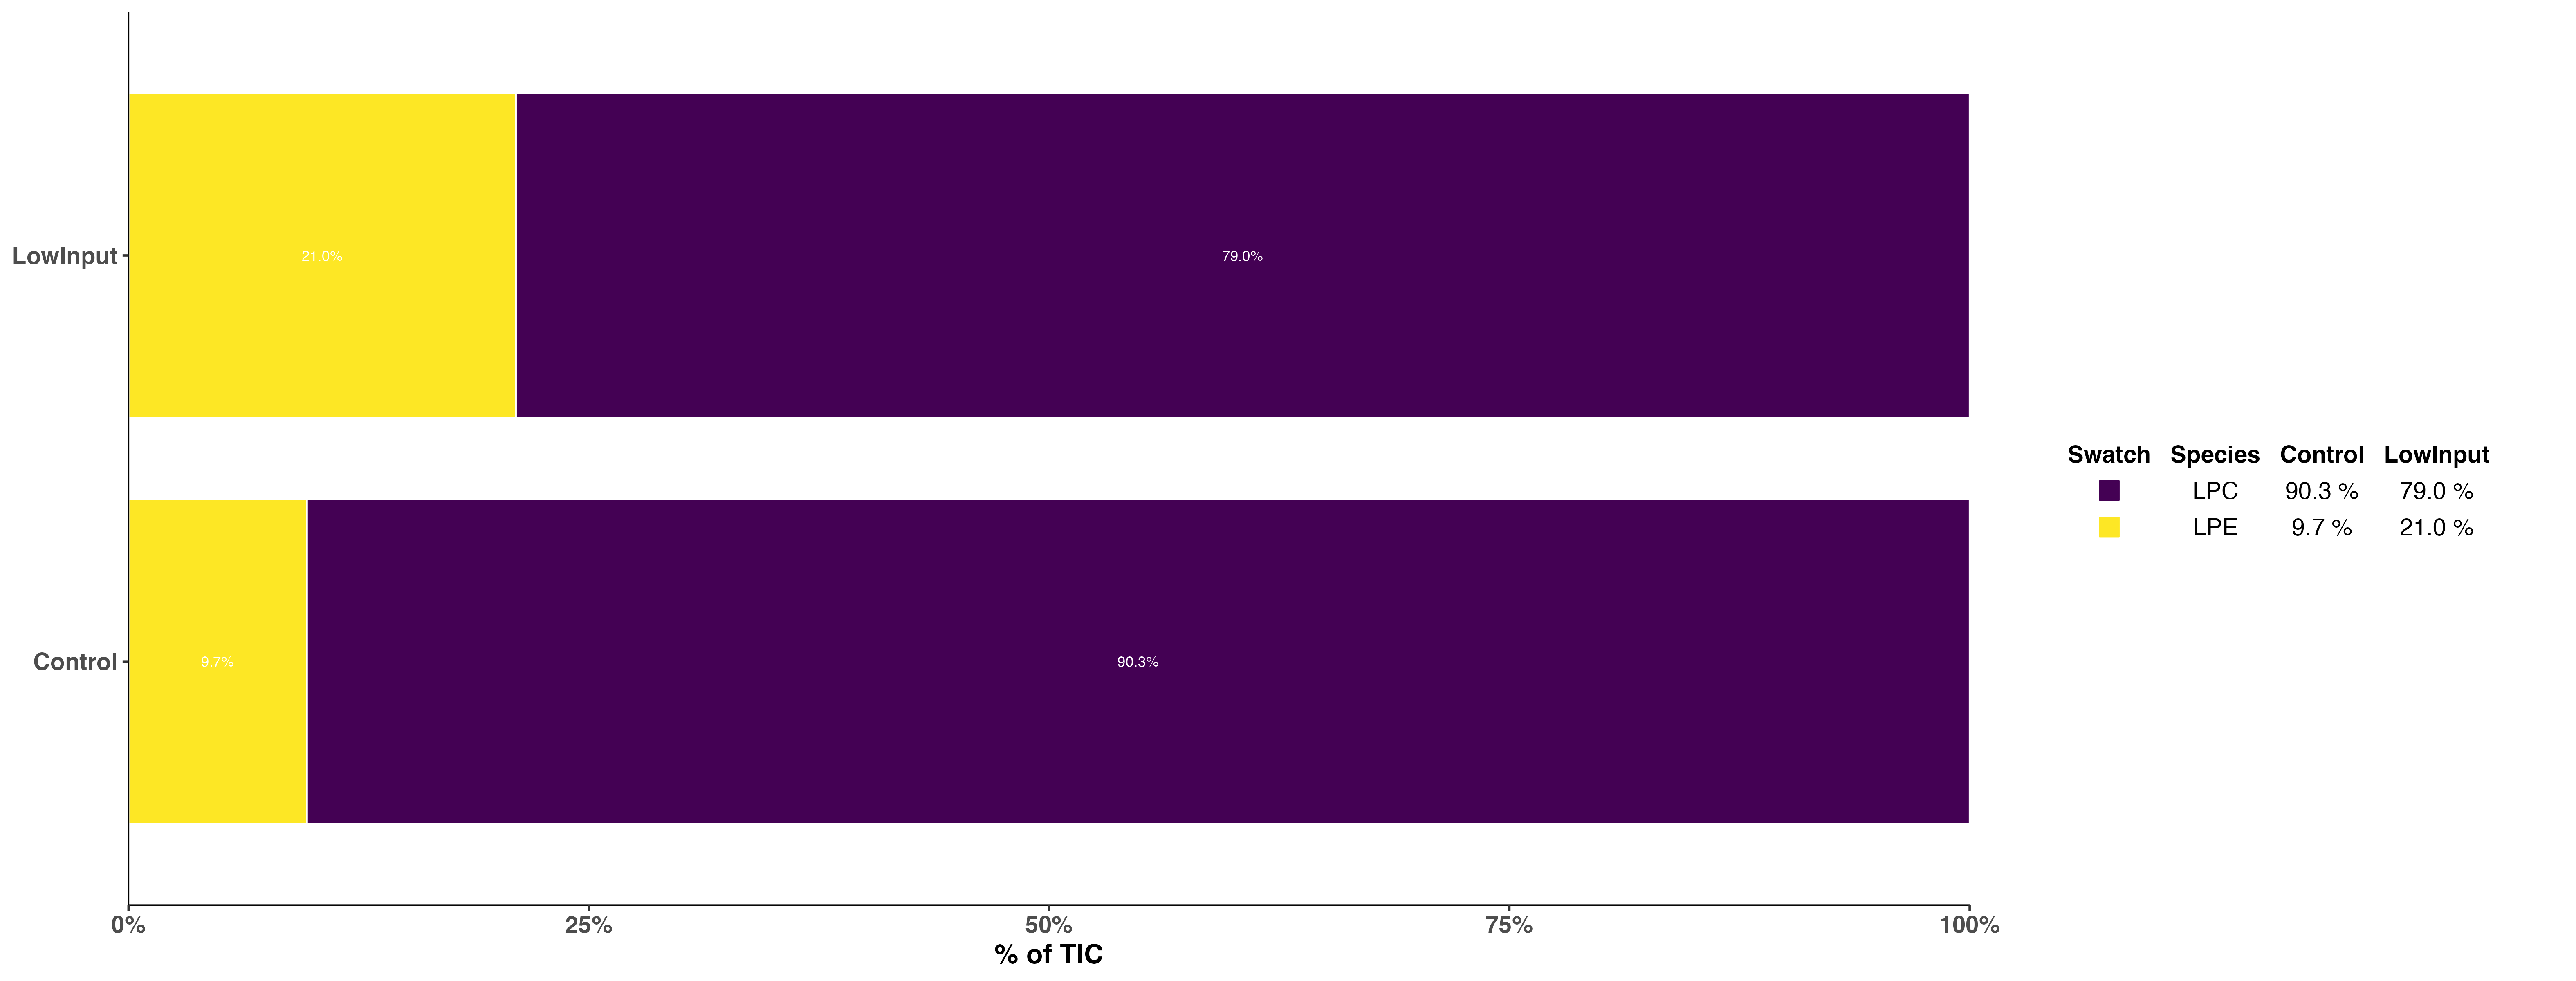
\includegraphics[width=0.7\textwidth]{fig/supp/SuppFig_5_TIC_LPC_LPE.png}
  \caption{Total ion current (TIC) proportions of lysophosphatidylcholine (LPC) and lysophosphatidylethanolamine (LPE) under Control and Low-P conditions. The plot displays relative TIC share of LPC versus LPE; stars denote significance levels (e.g., *: $p<0.05$, **: $p<0.01$) from appropriate tests. An increase in the LPE fraction and corresponding decrease in LPC under low-P suggests selective deacylation of PE for P salvage, while PC-derived LPC remains relatively stable.}
  \label{fig:S5_TIC_LPC_LPE}
\end{figure}



\end{document}


